\documentclass[12pt]{report}


% Macro definitions, packages
\input{defs.tex}

% Bib info
\usepackage{cite}
% \addbibresource{resources.bib}
% \usepackage[margin=0.7in]{geometry} % 1in for Umich
\usepackage[margin=1.0in]{geometry} % 1in for Umich
\setcounter{errorcontextlines}{50}

\title{\titleName}
\author{Aaron White}

% \setstretch{0.9} % 1.5 for Umich
\onehalfspacing



\begin{document}

\pagenumbering{gobble}
\begin{titlepage}

\begin{center}
\phantom{x}\\
\vspace{10em}
\textbf{\Large\titleName}\\
\vspace{5em}
by\\
Aaron White\\
\vspace{5em}
{\singlespacing
A dissertation submitted in partial fulfillment\\
of the requirements for the degree of\\
Doctor of Philosophy\\
(Physics)\\
in The University of Michigan\\
2021\\
}
\end{center} 

\vspace{5em}
{\singlespacing
\noindent Doctoral Comittee:\\
\phantom{xxxx} Professor Bing Zhou, Chair \\
\phantom{xxxx} Professor Christine Aidala\\
\phantom{xxxx} Professor David Baker\\
\phantom{xxxx} Professor Tom Schwarz\\
\phantom{xxxx} Professor James Wells\\
}

\end{titlepage}

\clearpage

\begin{center}
\doublespacing
\vspace*{\fill}
\href{http://hg8i.com/thesis/}{Aaron White} \\
aaronsw@umich.edu \\
ORCID iD: 0000-0003-0714-1466 \\
\vspace{3em}
\textcopyright Aaron White 2021
\vspace*{\fill}
\end{center}

\thispagestyle{empty}


\pagenumbering{roman}
\cleardoublepage
\phantomsection
\addcontentsline{toc}{chapter}{Dedication}
\phantom{x}\\
\phantom{x}\\
\vspace{1.1em}

\begin{center}
\textbf{\LARGE Dedication}
\end{center}

% \vspace*{\fill}
\begin{center}
\emph{To my grandfather, Dr. David White}
\end{center}
% \vspace*{\fill}


\cleardoublepage
\phantomsection
\addcontentsline{toc}{chapter}{Acknowledgements}
\phantom{x}\\
\phantom{x}\\
\vspace{1.1em}

\begin{center}
\textbf{\LARGE Acknowledgements}
\end{center} 

First I would like to thank my mother, Judith White, and my siblings David White, Ben White, and Laura White, for their love and support.

I am deeply indebted to the many educators who, during the past twenty one years, have through generosity and patience exposed me to knowledge and taught me how to learn.
First I am thankful to my high school teachers John Donnelly and Eric Dennison for teaching me calculus and computer programming, and Dan Falcon, John Phipps, and Sally Hair for encouraging me to study science.
I want to thank Dartmouth College professors John Thorstensen, Robert Caldwell, and James LaBelle for introducing me to physics and astronomy.
I would also like to thank George O'Toole, Kyle Cady, and John Hammond for involving me with research during this time.

There are many University of Michigan professors that I would like to thank;
Jean Krisch for her guidance;
Dragan Huterer for teaching me introductory physics and supervising me as a freshman;
Sally Oey for teaching me stellar dynamics and supervising me in research as a sophomore;
Christine Aidala for introducing me to high energy experimental physics and supervising me in research as a junior and senior and, along with Leopoldo Pando Zayas, teaching me mathematical methods;
Michael Zieve for teaching me analysis;
Bing Zhou, Roberto Merlin, and James Liu for teaching me the most elegant of theories, electromagnetism;
Bing Zhou again, along with Aaron Leanhardt and Junjie Zhu for teaching me classical mechanics;
Jianming Qian, Tom Schwarz, and Carl Akerlof for teaching me experimental methods;
James Wells, Henriette Elvang, and Ratindranath Akhoury for teaching me quantum field theory.

I have benefited from the help and generosity of many people during my time working on this project.
I would like to thank the members the ATLAS Collaboration who have built and run the detector and computing infrastructure that has enabled my work.
Their work and mine has been supported by various national funding agencies including the Department of Energy.
I would also like to thank the engineers and staff at CERN who help operate the LHC and maintain the site and the ATLAS secretaries who have helped solve numerous problems that occur as a result of living in France.
I am thankful to the Michigan ATLAS group professors Bing Zhou, Jianming Qian, Tom Schwarz, Dan Amidei, Junjie Zhu, Jianming Qian, Homer Neal, and Jay Chapman, as well as Tiesheng Dai, for building a supportive university environment and attracting the funding that has enabled this work.
I am also thankful to faculty of the Laboratoire de l'Acc\^el\^erateur Lin\^eaire and especially Louis and Lydia Fayard.
I am thankful to the friends I have made through physics for engaging in interesting discussions, especially Tom Cheng, Yicheng Guo, Zhi Zheng, Zirui Wang, Rongkun Wang, Zhongyukun Xu, and Siyuan Sun, Yanlin Liu, Aishik Gosh, Aaron White, Ismet Siral, Corentin Allaire, Hao Liu, and Dan Marley.
In particular, Matthew Klein has provided patient and invaluable guidance on topics of data analysis.
During my authorship qualification, I benefited from the guidance of Tom Schwarz and technical instruction of Xueye Hu, Jinhong Wang, and Bob Ball.
On the search for the Higgs decay to two muons, I am thankful for the guidance of Yusheng Wu, Yanlin Liu, and Bing Li.
On the search for contact interactions, I would like to thank the Exotics-LPX Dilepton group and our ever patient editorial board, Paul de Jong, Ulla Blumenschein, and Elliot Lipelles for their feedback.
I would especially like to thank Uta Klein, Dan Hayden, Etienne Dreyer, Peter Falke, Tanya Hryn'Ova, Sean Lawler for their contributions and guidance, and Stephan Hageboeck for his statistical input.
I am thankful for the LPX and Exotics group leadership of Yasu Okumura, Nikolina Llic, Antonio Sidoti, Carl Gwilliam, and Oliver Stelzer-Chilton.
I want to remark on my great fortune to have worked on this project with Deshan Abhayasinghe and Noam Tal Hod, who have made the this project one of the highlights of the past five years.
I am thankful for the committee, Bing Zhou, Tom Schwarz, Christine Aidala, James Wells, and David Baker for reviewing this thesis.
Finally, I want to extend my deepest thanks to my advisor, Bing Zhou.
She has worked tirelessly to support me since, as an undergraduate, I enrolled in her section of Physics 405: Intermediate Electromagnetism.
As a role model, her persistent curiosity and attention to detail have provided an exceptional example to follow of an experimental physicist. 
As a mentor, she has always pushed me to work to my fullest ability.



\cleardoublepage
\phantomsection
\tableofcontents
\cleardoublepage
\phantomsection
\addcontentsline{toc}{chapter}{List of Figures}
\listoffigures
\cleardoublepage
\phantomsection
\addcontentsline{toc}{chapter}{List of Tables}
\listoftables
\cleardoublepage
\phantomsection
\addcontentsline{toc}{chapter}{List of Appendices}
\renewcommand{\thesection}{\Alph{section}}
\listofappendices
\cleardoublepage
\phantomsection
\addcontentsline{toc}{chapter}{Abstract}
\phantom{x}\\
\phantom{x}\\
\vspace{1.1em}

\begin{center}
\textbf{\LARGE Abstract}
\end{center} 

This thesis presents two topics: a search for rare dimuon decay of the Standard Model Higgs boson and a search for new physics with non-resonant phenomena at the TeV mass scale with dilepton final states.
Both studies investigate data recorded by the ATLAS experiment from $\sqrt{s}=13$~TeV proton-proton collisions produced during the second of the Large Hadron Collider at CERN.
This data corresponds to an integrated luminosity of 139~fb$^{-1}$. 
% Both studies investigate an integrated luminosity of 139~fb$^{-1}$ of data recorded by the ATLAS from $\sqrt{s}=13$~TeV proton-proton collisions from Run~2 of the Large Hadron Collider at CERN.

The first study is the search for the Standard Model Higgs boson decaying to two muons.
This decay is used to study the Higgs boson Yukawa couplings to the second generation fermions as part of a field-wide effort to study the properties of the Higgs boson.
Identifying events produced by this decay is complicated by the small Higgs boson branching fraction to muons and the large irreducible background from other Standard Model processes.
% The major Higgs production modes at the LHC are gluon-gluon fusion (ggF), vector-boson fusion (VBF), a vector boson (W or Z) associated production (VH).
Previous studies selected events using criteria that targets Higgs production through gluon-gluon fusion and vector-boson fusion mechanisms.
To increase sensitivity to Higgs produced events, new selections are added targeting vector boson associated (VH) production with a leptonic decay from the vector boson.
Multivariate analysis methods are used to identify events for different categories.
The limits set on signal production in the new phase spaces explored in this analysis are the first of their kind.
The strongest expected (observed) limit on leptonic VH production excludes signals down to 13.2 (22.6) times the Standard Model prediction.
The combination of VH with the other major production modes results in a signal significance of 2.0$\sigma$ over the background hypothesis.

The second study is a search for non-resonant phenomena in the dielectron and dimuon final states.
One possible source for this is quark and lepton compositeness at energy scales beyond direct access at the LHC.
These would lead to contact interactions that produce non-resonant enhancement in dilepton production at the TeV mass scale.
This search introduces several novel methods including a background model derived from data and a formalism to parameterization of the associated uncertainties.
% This is done in a low-mass control region where the signal is expected to be negligible, while the function is extrapolated to several high-mass signal regions where an enhancement of events is expected above the background processes.
% This approach mitigates the statistical and theoretical uncertainty of simulated background predictions.
In this search, no significant deviation in data is observed with respect to the expected background.
Upper limits on the visible cross-section times branching ratio are set in this search.
These, along with benchmark CI signal efficiencies, can be interpreted as limits in terms of a variety of signal models.
The lower limits on the energy scale of CI, $\Lambda$, reach 35.8 TeV, indicating the quarks and leptons are still point-like particles at 10$^{-20}$ m.
These are the strongest limits on \qqll contact-interactions to date.


\cleardoublepage


\pagenumbering{arabic}
% \addtocontents{toc}{%
% \protect\contentsline{part}{Chapters}{}}
% \addtocontents{toc}{\protect\contentsline{chapter}{\protect Chapters}{}{}}
\addcontentsline{toc}{part}{Chapters}

% \chapter{Introduction}

% Experimental observations are the foundations of the our knowledge of these building blocks.
% The most complete mathematical description of these building blocks based, on experimental knowledge, is the Standard Model of particle physics.


% Particles
The Universe consists of particles, the space they inhabit, and the interactions between them.
Fundamental particles are the most basic unit of matter, with observable properties including mass, charge couplings, spin, and lifetime.
Particles with integer spins are called bosons, while particles with half-integer spins are called fermions.
Particles may be composite, such as the proton, or elementary, as is assumed for the electron.
Particles and the interactions between them together form the physical world.
The most complete mathematical description of these building blocks, based on experimental knowledge, is the Standard Model (SM) of particle physics.
This theory has evolved and expanded since original development in 1974, with each iteration encompassing the consensus view of the physics community.
% The Standard model describes particles at the most fundamental, with no internal substructure.

% Added by Bing
This dissertation presents research on the nature of particle physics conducted at the Large Hadron Collider with the ATLAS experiment. 
The basic principles of particle physics are introduced in this chapter, followed by the particular research topics of this thesis.

\section{Particles, Space, and Interactions}

% Fermions
Each type of fermion exists in a pair, consisting of \emph{particles} and \emph{anti-particles} with equal mass and opposite electric charges.
The fermions are further divided into leptons with integer electric charge and quarks with fractional electric charges.
There are three \emph{flavors} of charged leptons. In ascending mass these are the electron, the muon, and the tauon.
There are also three flavors of neutral leptons, corresponding to each charged lepton flavor, called neutrinos.
Recent measurements provide an indication that the neutrino masses are ordered similarly to the order of charged leptons \cite{kamio}.
The leptons are arranged into three \emph{generations} based on the approximate conservation of the number of leptons minus the number of anti-leptons belonging to each generation in a given interaction.
There are six quarks, divided into up-type quarks and down-type quarks.
The up-type quarks are the up, charm, and top quarks.
The down-type quarks are the down, strange, and bottom quarks.
Like the leptons, up- and down-type quarks are paired together in generations of ascending mass.
Quarks commonly exist in bound-states consisting of two (meson) and three (baryon) quarks.
% Bosons
The bosons mediate forces between the particles.
The most familiar boson, the photon, mediates the electromagnetic force between charged particles.
The gluons carry the strong nuclear force, binding quarks inside multi-quark composite particles called hadrons.
The \W and \Z bosons carry the weak nuclear force, responsible for nuclear beta decays.
These bosons are called \emph{vector gauge bosons} because of their association with gauge groups.
Finally, the recently discovered scalar particle, the Higgs boson, mediates a momentum exchange between massive particles.
% Summary
These particles are summarized in Table \ref{tab:particles}.

\begin{table}[htp]
\begin{center}
\caption{Particles of the Standard Model listed along with their symbol and several properties \cite{pdg2018}. ($^*$ The graviton is not considered part of the SM.)}
{\footnotesize
\begin{tabular}{c c l c l c c c c c c}
\toprule
& & Name & Symbol & \multicolumn{1}{c}{Generation} & Charge & Spin & Mass [MeV/c$^2$] \\
\midrule
\multirow{12}{*}[0em]{\begin{sideways}Fermions\end{sideways}} & \multirow{6}{*}[0em]{\begin{sideways}Leptons\end{sideways}} & Electron & \e & ~~~~~~\first & -1 & 1/2 & 0.511 \\
& & Muon   			  & \m         & ~~~~~~\second & -1 & 1/2 & 105.7 \\
& & Tau    			  & $\tau$     & ~~~~~~\third  & -1 & 1/2 & 1776.8 \\
& & Electron Neutrino & $\nu_e$    & ~~~~~~\first  & 0  & 1/2 &  $<2\times10^{-6}$\\
& & Muon Neutrino     & $\nu_\mu$  & ~~~~~~\second & 0  & 1/2 &  $<2\times10^{-6}$\\
& & Tau Neutrino      & $\nu_\tau$ & ~~~~~~\third  & 0  & 1/2 &  $<2\times10^{-6}$\\
\cline{2-8}
& \multirow{6}{*}[0em]{\begin{sideways}Quarks\end{sideways}} & Up & $u$ & ~~~~~~\first & 2/3 & 1/2 &  $2.2\pm0.5$ \\
& & Charm             & $c$ & ~~~~~~\second &  2/3 & 1/2 &  $1.275\pm0.035\times10^{3}$ \\
& & Top               & $t$ & ~~~~~~\third  &  2/3 & 1/2 &  $173.0\pm0.4\times10^{3}$ \\
& & Down              & $d$ & ~~~~~~\first  & -1/3 & 1/2 &  $4.7\pm0.5$ \\
& & Strange           & $s$ & ~~~~~~\second & -1/3 & 1/2 &  $95\pm9$ \\
& & Bottom            & $b$ & ~~~~~~\third  & -1/3 & 1/2 &  $4.18\pm0.04\times10^{3}$ \\
\midrule
\multicolumn{2}{c}{\multirow{6}{*}[0em]{\begin{sideways}Bosons\end{sideways}}} & Photon & $\gamma$ && 0 & 1 & $<1\times10^{-24}$ \\
& & Gluon         & $g$ & & 0 & 1 & 0 \\
& & Z boson       & \Z  & & 0 & 1 & $91.1876\times 10^3$ \\
& & W boson       & \W  & & $\pm$1 & 1 & $80.39\times 10^3$ \\
& & Higgs boson   & \h  & & 0 & 0 & $125.18\times 10^3$ \\
& & Graviton$^*$  & $g$ & & 0 & 2 & $<1\times 10^{-38}$ \\
\bottomrule
\end{tabular}
}
\label{tab:particles}
\end{center}
\end{table}

While the Standard Model has been successful in the description of particles and their interactions, it is an incomplete description of the Universe.
The most visible shortcoming is the lack of a description of gravity; the quantum effects of gravity are expected to manifest themselves at energy scales that are inaccessible to modern particle experiments.
Other absences in the theory include particles that explain the phenomena of dark matter and dark energy.
The theory also lacks a single broadly accepted explanation for the mass of neutrinos, although several plausible mechanisms have been proposed \cite{jw2019}.
Ongoing experiments are investigating discrepancies between predicted and observed quantities, such as the anomalous magnetic moment of the muon.
Despite these absences the present version of the Standard Model is a remarkably predictive theory.

% \section{Spacetime}

Spacetime is the four-dimensional manifold that particles inhabit at a microscopic scale.
Three of these are spacial dimensions, and one is time: 3+1-dimensional spacetime.
The special theory of relativity describes the distinction between the dimensions: rotations from one spacial dimension to another take place in Euclidean space, while rotations from a spatial dimension into time take place in a hyperbolic space.
None of this should be taken at face value, or as posed by Ehrenfest in 1917, \emph{in what way does it become manifest in the fundamental laws of physics that space has three dimensions?}
One point to consider is the stability of elliptical orbits in a two-body system.
If the number of space dimensions exceeds three, then stable circular orbits under gravity are impossible.
This result holds for the quantum orbits of electrons around a nucleus as well.
Therefore if one is to find oneself in a universe with atoms, chemistry, and planets, then the number of spatial dimensions in which these take place is limited to three~\cite{ehrenfest}.
This limit on space dimensions suggests the question: why one time dimension?
In the case of multiple time dimensions, solutions to partial differential equations such as those that describe the laws of physics are ambiguous.
This is analogous to the situation in 3+1-dimensional spacetime wherein predictions outside the lightcone are impossible.
It has been argued by Tegmark that this precludes observers, as the lack of predictability renders reality incomprehensible~\cite{tegmark-time}.


% \section{Interactions}
Until the discovery of the Higgs boson, there were four known fundamental forces through which particles might interact: gravity, the electromagnetic force, the weak nuclear force, and the strong nuclear force.
An interaction between two or more particles entails the exchange of momentum between the participants.
For each force, the momentum exchange is mediated by a boson.
Gluons mediate the strong nuclear force.
The weak nuclear force is mediated by the \Wp, \Wm, and \Z bosons.
Photons mediate the electromagnetic force.
It is expected that gravity is mediated by a hypothetical particle called a graviton; however, this has not been observed. The gravitational interaction strength is more than an order of 40 magnitude smaller compared to the electromagnetic interaction. At the microscopic level, the interaction of the gravity could be ignored and is not included in the Standard Model.

In 2012, the ATLAS and CMS experiments at the Large Hadron Collider at CERN discovered the Higgs boson. Like the vector bosons associated with the four canonical forces, the scalar particle, Higgs boson, mediates a momentum exchange between particles. The interactions with fermions are not universal, proportional to fermion's mass.

\begin{table}[htp]
\begin{center}
\caption{Interactions in experienced by particles. The strength of the force depends on the energy scale at which it is measured, so approximate values are given \cite{robinson}. In the case of Gravity, which is not included in the Standard Model, the coupling strength is assumed to be on the order of the gravitational constant \cite{donogue}.}
{\normalsize
\begin{tabular}{c c l c c c c c c c}
\toprule
Interaction            & Force Carrier &  Relative Strength   & Range [m]  \\
\midrule
Strong           & Gluon      &  1           & $10^{-15}$ \\
Electromagnetic  & Photon     &  $10^{-2}$   & $\infty$   \\
Weak             & \W, \Z     &  $10^{-5}$   & $10^{-18}$ \\
Higgs            & Higgs      &  $<10^{-5}$  & $10^{-19}$ \\
Gravity          & Graviton   &  $ 10^{-39}$ & $\infty$   \\
\bottomrule
\end{tabular}
}
\label{tab:forces}
\end{center}
\end{table}

\section{Energies and Measures}

Enormous energy concentrations are required to enable the production of massive particles and facilitate rare interactions.
In order to study these processes, it is convenient to define units of measurements using energy as the basic unit to describe the particle mass, momentum, lifetime, and travel distance.

Energies are measured in units of \emph{electron-volts}, eV.
This is equal to the energy required to move an electron through one volt of electric potential.
One eV is a small amount of energy, equivalent the amount needed to move a single electron from one terminal of a AA battery to the other.
In the scope of discovered particles and interactions, eV are often presented along with metric prefixes.
One mega-electronvolt (MeV) is one million eV, and is the energy scale reached by the earliest circular particle accelerators with fixed magnetic fields called cyclotrons.
One giga-electronvolt (GeV) is one billion eV, and became accessible with the development of synchrotron accelerators that gradually increased their fields to reach higher energies.
One tera-electronvolt (TeV) is one trillion eV.
The stack of AA batteries required to accelerate an electron to 1 TeV would reach from Earth to Mars at its closest approach.
Although the Tevatron at Fermilab came close, the TeV scale was first reached at the Large Hadron Collider (LHC) at CERN.
The energy at the LHC subsequently accelerated protons to energies of 7~TeV.
The particular energy scales of interest in this thesis range from tens of GeV to tens of TeV.

Several quantities are useful in describing interactions between particles: energy, mass, momentum, distance, and time.
The unit of eV already describes quantities of energy.
In standard international (SI) units, energy is measured in units of joules (J) equal to kg$\frac{\text m^2}{\text s^2}$.
Mass is, therefore, expressible as energy divided by velocity squared.
A convenient velocity to use is the speed of light, $c$.
In this case, mass is expressed in units of GeV/$c^2$.
Likewise, momentum, which is measured in SI units as kg$\frac{\text m}{\text s}$, can be expressed in units of GeV/$c$.
Distance and time can be expressed with the aid of the reduced Planck's constant $\hbar=6.58\times10^{-25}~$GeV$\cdot$s.
Using $\hbar$, distance is measured in units of $\hbar c/$GeV, and time is measured in units of $\hbar/$GeV.
These are referred to as \emph{Planck units} and are commonly used throughout this thesis along with SI units following the field's standard practice.
In cases where their presence can be inferred from the quantity, the SI units are replaced such that the constants $\hbar$ and $c$ have numerical values of 1, leaving powers of GeV.
These units are summarized in Table \ref{tab:units}.

\begin{table}[htp]
\caption{Description of the units used to describe dimensions in this thesis. Each row lists equivalent quantities.}
\begin{center}
\begin{tabular}{l l l l l l}
\toprule
Dimension & SI Units &  Planck Units & Natural Units \\
          &          &               & $c=1$, $\hbar = 1$ \\
\midrule
Energy    &    1.602$\times10^{-10}$J               & ~~~~GeV            & ~~~~GeV \\
Mass      &    1.783$\times10^{-27}$kg              & ~~~~GeV/$c^2$      & ~~~~GeV \\
Momentum  &    5.344$\times10^{-19}$kg$\cdot$m/s    & ~~~~GeV/$c$        & ~~~~GeV \\
Distance  &    1.973$\times10^{-16}$m               & ~~~~$\hbar c/$GeV  & ~~~~GeV$^{-1}$ \\
Time      &    6.582$\times10^{-25}$s               & ~~~~$\hbar/$GeV    & ~~~~GeV$^{-1}$ \\
\bottomrule
\end{tabular}
\label{tab:units}
\end{center}
\end{table}

The probability that two marbles rolled towards each other will collide is proportional to their respective cross-sectional areas, called cross-sections.
Likewise, the probability of a particular interaction between particles is measured in units of area.
The unit \emph{barn} is defined such that 1b=$10^{-28}\text m^2$.
It was named during the Manhattan Project by Marshall Holloway and C. P. Baker; the two rejected the idea of naming the unit after John Manley due to the ``use of the term for purposes other than the name of a person'' \cite{holloway}.
As the progenitors remark, the barn is quite a large area to describe particle interactions.
Therefore prefixed versions like picobarn ($1\text{pb}=10^{-12}$b) and femptobarn ($1\text{fb}=10^{-15}$b) are commonly used in colliding beam experiments.
The barn is essentially an SI unit. If it were to be expressed in the natural units of Table \ref{tab:units}, it would be approximately equal to $2568\frac{\hbar^2 c^2}{\text{GeV}^2}$.

% Symbols
Throughout this thesis numerous quantities are calculated from observations.
Perhaps the most central quantity is \emph{invariant-mass}, defined as the squared energy minus the squared momentum of a system.
For a system containing a single particle, the invariant-mass measured in any inertial reference frame of motion is identical to the particle's mass measured at rest.
This thesis is primarily concerned with systems of two component particles, such as the dielectron and dimuon systems.
In such systems the energy, $E$ is defined by the scalar sum of the components' energy and the momentum, $\vec{p}$, as the vectorial sum.
The invariant-mass of dielectron, dimuon, or dilepton systems is denoted as \mee, \muu, or \mll depending on the context.
Other common quantities refer to transverse measurements perpendicular the path of colliding beams, \zhat.
The first is \emph{transverse momentum}, \vecpt, which is a 2-vector defined as a system's momentum perpendicular \zhat.
The magnitude of \vecpt is labeled \pt.
Other transverse quantities include \emph{transverse mass}, $\mt\equiv \sqrt{E^2-p_z^2}$, and the vectorial \emph{transverse energy}, $\vec{E}_\text{T}\equiv=E\frac{\vec{p}_\text{T}}{|\vec{p}|}$.

\section{Two Analyses}
% ATLAS and data
This thesis presents two studies based on data collected by the ATLAS experiment at the Large Hadron Collider based at CERN.
These studies analyze data recorded from collisions of proton beams with a center-of-mass energy of $\sqrt{s}=13$~TeV.
Each collision of interest, or event, is recorded and studied in order to extract information about the underlying interactions involved with the collision. 
The first study is concerned with the predicted interaction of the Higgs boson with pairs of muons.
The second study searches for enhancements in the production of energetic pairs of leptons (dileptons) as predicted by extended theories beyond Standard Model. 

The unifying theme of these analyses is their focus on the production of leptons in their final state.
In both cases the final discriminant variable, from which a measurement is extracted, is the invariant-mass of a dilepton pair. 
The similarity ends here, with different physics goals and theoretical models distinguishing each effort.

\subsection{Search for the Higgs decay to Two Muons}
% \cite{jw2019}
The first study presented in this thesis relates to the Higgs boson.
The Higgs boson was discovered in 2012 by the ATLAS and CMS collaborations \cite{atlashiggs,cmshiggs}.
This discovery provided the impetuous for subsequent study of the new particle.
A concerted effort has been made to measure the properties of the Higgs boson, with a particular focus on measuring its interactions with the rest of the Standard Model particles.
The first interactions were measured using the Higgs coupling to the gauge bosons and the heaviest fermions.
This work is aided by the relatively large coupling to heavier particles than to lighter particles.
At the time of writing, the lightest particle for which there is evidence of its direct coupling to the Higgs is the tau lepton ($m_\tau=1.8$~GeV).

The first focus of this thesis is to search for a presently unobserved interaction of the Higgs boson with muons.
This interaction is interesting from two perspectives.
First, unlike previously measured Higgs interactions, this coupling involves second generation fermions.
This is important as a test of Higgs properties with a new sector of particles.
Second, this interaction is produces fermion mass and is consequently an important property of the muon. 
The muon, with a mass of $m_\mu=0.1$~GeV, is a relatively light fermion. As a result, the strength of its coupling to the Higgs boson is relatively weak.

% Previous work.
The search for evidence of the \hmm process has attracted significant attention since the Higgs discovery.
Despite the efforts of both the ATLAS and CMS collaborations, it has yet to be detected with a significance meeting the threshold of 3$\sigma$.
These searches focuses on the decay of the Higgs boson to a muon/anti-muon pair (\hmm).
They consider events that produce two oppositely charged muons in their final state.
The previous work by both collaborations has investigated partial datasets produced before the completion of Run~2.
These studies set upper limits on the strength of the interaction, but are not sensitive enough to report significant evidence \cite{atlasHmm36,cmsHmm35}.

The study presented in this thesis offers an iteration on these past efforts, as well as the first examination of the full Run~2 dataset.
A major challenge faced in this analysis is the separation of signal events producing a Higgs boson from background events that lack a Higgs.
Several strategies are employed that distinguish this iteration from prior results.
The first improvement is to expand the scope of the analyzed data to include Higgs bosons produced by previously unconsidered processes.
The most significant of these is ``Higgs produced in association with a vector boson'' (VH); this mechanism produces a vector boson in addition to the Higgs.
The additional vector boson is useful to help discriminate the VH process from background processes.
A new categorization scheme is employed to study these events.
Many of the event topologies produced by these new production mechanisms have never been studied before.
A second improvement is in the use of multivariate discriminants to label events as signal-like or background-like. 
The type of discriminant used is an ensemble of decision trees, called a \emph{boosted decision tree}, that categorize events based on quantities measured by the detector.
This iteration of the analysis expands the use of multivariate discriminants and introduces robust model validation techniques to constrain biases introduced by their use.

For each event that is considered, the invariant-mass of the Higgs candidate dimuons is calculated based on measured energies and momenta of selected two muons.
These form several spectra of invariant-mass, with each spectrum corresponding to a particular selection of events.
Background production mechanisms produce a monotonically decreasing spectrum, while events produced by a \hmm process produce a narrow resonant shape in the spectrum.
Statistical tests are performed to measure the size and significance of this resonance above the smoothly falling background.

The results of this analysis are significant for two reasons.
First, they represent the first observations of phase spaces related to the newly considered Higgs production mechanisms.
Second, they represent the complete result for \hmm using the ATLAS Run~2 dataset.
Together this an analysis provides a blueprint for subsequent studies based on anticipated data from a future Run~3.
The results will also be combined with other studies of the Higgs boson to produce a more complete understanding of the boson's properties.

\subsection{Search for Non-resonant Signatures and Contact Interactions}
The second study presented in this thesis searches for the production of dileptons beyond the Standard Model prediction.
This strategy stands in contrast to the search for \hmm, which targets a signal predicted by the SM.
The analysis searches for broad \emph{non-resonant} phenomena in the dilepton invariant-mass spectrum without constraining the specific source of the production.
The target of this study is distinguished from the narrow spectral resonances, such as those searched for in the \hmm analysis.

A wide variety of new physics models predict non-resonant phenomena.
A particularly interesting group of theories are contact interactions; these describe the effective behavior of new energetic interactions at a relatively low energy.
These new interactions can be facilitated by a yet-undiscovered heavy boson.
Contact interactions may also be an indication of unexpected sub-structure within fermions.
For these varied reasons, contact interactions have attracted substantial experimental interest for decades \cite{eichten,zeusCi,alephCi}.

The search presented in this thesis expands on previous results by the ATLAS collaboration \cite{EXOT-2016-05,EXOT-2015-07,EXOT-2013-19,EXOT-2012-17}.
It is carried out in two channels: a dielectron channel and a dimuon channel.
The final discriminant variable is the dilepton invariant-mass in each respective channels.
The search focuses on the highest mass events in the dilepton invariant-mass spectra.
As a result, the focus of the analysis is the description of the spectrum tails and the associated uncertainties of those descriptions.

As in the case of the search for \hmm, this study benefits from the unprecedented size of the full Run~2 dataset.
Further improvements offer a dramatic departure from prior efforts.
A new method is introduced to describe the expected invariant-mass spectrum based on a functional form fit to the observed data in a low invariant-mass control region.
This function is then extrapolated to higher invariant-mass to describe the background. 
This novel background model necessitated the development of new types of systematic uncertainty.

Perhaps the most impactful development of this analysis is the identical treatment of events above a certain invariant-mass thresholds.
These are counted without reference to their energy.
As a result, the observed yield of events can be interpreted in terms of a wide variety of signal models that predict differently shaped contributions to the dilepton invariant-mass spectra.
A detailed comparison of the sensitivity expected from including and ignoring the spectral shape found no significant cost to adopting this strategy. 

The observations of the analysis are interpreted both in terms of contact interactions and from a signal model-independent perspective.
The contact interaction results probe an enormous energy scale at tens of TeV.
The model-independent results represent the first such results for a non-resonant search in the high-mass spectrum.

% Summary
\section{Organization}

The topic of this thesis is two studies related to the production of dilepton events.
Both studies are informed by the theoretical predictions of the Standard Model.
Furthermore, both are conducted using the data recorded by the ATLAS experiment at the LHC.
In light of these commonalities, the first chapters of this thesis present the common background for each study.
Chapter \ref{sec:theory} presents the Standard Model.
Chapter \ref{sec:experiment} describes the ATLAS experiment, the LHC, and the data collection.
Chapter \ref{sec:phenomenology} discusses the phenological basis for studying physics at the LHC.
Chapter \ref{sec:objectsDatasets} describes the details of the datasets used for both studies.
Next, separate chapters present the specific details of each study.
Chapter \ref{sec:hmumu} presents the study of the Higgs boson's interaction with muons.
Chapter \ref{sec:ci} presents the search for contact interactions and related phenomena.
Finally, Chapter \ref{sec:summary} summarises the results of both studies and discusses the prospect for future work.




\chapter{Introduction}

% Experimental observations are the foundations of the our knowledge of these building blocks.
% The most complete mathematical description of these building blocks based, on experimental knowledge, is the Standard Model of particle physics.


% Particles
The Universe consists of particles, the space they inhabit, and the interactions between them.
Fundamental particles are the most basic unit of matter, with observable properties including mass, charge couplings, spin, and lifetime.
Particles with integer spins are called bosons, while particles with half-integer spins are called fermions.
Particles may be composite, such as the proton, or elementary, as is assumed for the electron.
Particles and the interactions between them together form the physical world.
The most complete mathematical description of these building blocks, based on experimental knowledge, is the Standard Model (SM) of particle physics.
This theory has evolved and expanded since original development in 1974, with each iteration encompassing the consensus view of the physics community.
% The Standard model describes particles at the most fundamental, with no internal substructure.

% Added by Bing
This dissertation presents research on the nature of particle physics conducted at the Large Hadron Collider with the ATLAS experiment. 
The basic principles of particle physics are introduced in this chapter, followed by the particular research topics of this thesis.

\section{Particles, Space, and Interactions}

% Fermions
Each type of fermion exists in a pair, consisting of \emph{particles} and \emph{anti-particles} with equal mass and opposite electric charges.
The fermions are further divided into leptons with integer electric charge and quarks with fractional electric charges.
There are three \emph{flavors} of charged leptons. In ascending mass these are the electron, the muon, and the tauon.
There are also three flavors of neutral leptons, corresponding to each charged lepton flavor, called neutrinos.
Recent measurements provide an indication that the neutrino masses are ordered similarly to the order of charged leptons \cite{kamio}.
The leptons are arranged into three \emph{generations} based on the approximate conservation of the number of leptons minus the number of anti-leptons belonging to each generation in a given interaction.
There are six quarks, divided into up-type quarks and down-type quarks.
The up-type quarks are the up, charm, and top quarks.
The down-type quarks are the down, strange, and bottom quarks.
Like the leptons, up- and down-type quarks are paired together in generations of ascending mass.
Quarks commonly exist in bound-states consisting of two (meson) and three (baryon) quarks.
% Bosons
The bosons mediate forces between the particles.
The most familiar boson, the photon, mediates the electromagnetic force between charged particles.
The gluons carry the strong nuclear force, binding quarks inside multi-quark composite particles called hadrons.
The \W and \Z bosons carry the weak nuclear force, responsible for nuclear beta decays.
These bosons are called \emph{vector gauge bosons} because of their association with gauge groups.
Finally, the recently discovered scalar particle, the Higgs boson, mediates a momentum exchange between massive particles.
% Summary
These particles are summarized in Table \ref{tab:particles}.

\begin{table}[htp]
\begin{center}
\caption{Particles of the Standard Model listed along with their symbol and several properties \cite{pdg2018}. ($^*$ The graviton is not considered part of the SM.)}
{\footnotesize
\begin{tabular}{c c l c l c c c c c c}
\toprule
& & Name & Symbol & \multicolumn{1}{c}{Generation} & Charge & Spin & Mass [MeV/c$^2$] \\
\midrule
\multirow{12}{*}[0em]{\begin{sideways}Fermions\end{sideways}} & \multirow{6}{*}[0em]{\begin{sideways}Leptons\end{sideways}} & Electron & \e & ~~~~~~\first & -1 & 1/2 & 0.511 \\
& & Muon   			  & \m         & ~~~~~~\second & -1 & 1/2 & 105.7 \\
& & Tau    			  & $\tau$     & ~~~~~~\third  & -1 & 1/2 & 1776.8 \\
& & Electron Neutrino & $\nu_e$    & ~~~~~~\first  & 0  & 1/2 &  $<2\times10^{-6}$\\
& & Muon Neutrino     & $\nu_\mu$  & ~~~~~~\second & 0  & 1/2 &  $<2\times10^{-6}$\\
& & Tau Neutrino      & $\nu_\tau$ & ~~~~~~\third  & 0  & 1/2 &  $<2\times10^{-6}$\\
\cline{2-8}
& \multirow{6}{*}[0em]{\begin{sideways}Quarks\end{sideways}} & Up & $u$ & ~~~~~~\first & 2/3 & 1/2 &  $2.2\pm0.5$ \\
& & Charm             & $c$ & ~~~~~~\second &  2/3 & 1/2 &  $1.275\pm0.035\times10^{3}$ \\
& & Top               & $t$ & ~~~~~~\third  &  2/3 & 1/2 &  $173.0\pm0.4\times10^{3}$ \\
& & Down              & $d$ & ~~~~~~\first  & -1/3 & 1/2 &  $4.7\pm0.5$ \\
& & Strange           & $s$ & ~~~~~~\second & -1/3 & 1/2 &  $95\pm9$ \\
& & Bottom            & $b$ & ~~~~~~\third  & -1/3 & 1/2 &  $4.18\pm0.04\times10^{3}$ \\
\midrule
\multicolumn{2}{c}{\multirow{6}{*}[0em]{\begin{sideways}Bosons\end{sideways}}} & Photon & $\gamma$ && 0 & 1 & $<1\times10^{-24}$ \\
& & Gluon         & $g$ & & 0 & 1 & 0 \\
& & Z boson       & \Z  & & 0 & 1 & $91.1876\times 10^3$ \\
& & W boson       & \W  & & $\pm$1 & 1 & $80.39\times 10^3$ \\
& & Higgs boson   & \h  & & 0 & 0 & $125.18\times 10^3$ \\
& & Graviton$^*$  & $g$ & & 0 & 2 & $<1\times 10^{-38}$ \\
\bottomrule
\end{tabular}
}
\label{tab:particles}
\end{center}
\end{table}

While the Standard Model has been successful in the description of particles and their interactions, it is an incomplete description of the Universe.
The most visible shortcoming is the lack of a description of gravity; the quantum effects of gravity are expected to manifest themselves at energy scales that are inaccessible to modern particle experiments.
Other absences in the theory include particles that explain the phenomena of dark matter and dark energy.
The theory also lacks a single broadly accepted explanation for the mass of neutrinos, although several plausible mechanisms have been proposed \cite{jw2019}.
Ongoing experiments are investigating discrepancies between predicted and observed quantities, such as the anomalous magnetic moment of the muon.
Despite these absences the present version of the Standard Model is a remarkably predictive theory.

% \section{Spacetime}

Spacetime is the four-dimensional manifold that particles inhabit at a microscopic scale.
Three of these are spacial dimensions, and one is time: 3+1-dimensional spacetime.
The special theory of relativity describes the distinction between the dimensions: rotations from one spacial dimension to another take place in Euclidean space, while rotations from a spatial dimension into time take place in a hyperbolic space.
None of this should be taken at face value, or as posed by Ehrenfest in 1917, \emph{in what way does it become manifest in the fundamental laws of physics that space has three dimensions?}
One point to consider is the stability of elliptical orbits in a two-body system.
If the number of space dimensions exceeds three, then stable circular orbits under gravity are impossible.
This result holds for the quantum orbits of electrons around a nucleus as well.
Therefore if one is to find oneself in a universe with atoms, chemistry, and planets, then the number of spatial dimensions in which these take place is limited to three~\cite{ehrenfest}.
This limit on space dimensions suggests the question: why one time dimension?
In the case of multiple time dimensions, solutions to partial differential equations such as those that describe the laws of physics are ambiguous.
This is analogous to the situation in 3+1-dimensional spacetime wherein predictions outside the lightcone are impossible.
It has been argued by Tegmark that this precludes observers, as the lack of predictability renders reality incomprehensible~\cite{tegmark-time}.


% \section{Interactions}
Until the discovery of the Higgs boson, there were four known fundamental forces through which particles might interact: gravity, the electromagnetic force, the weak nuclear force, and the strong nuclear force.
An interaction between two or more particles entails the exchange of momentum between the participants.
For each force, the momentum exchange is mediated by a boson.
Gluons mediate the strong nuclear force.
The weak nuclear force is mediated by the \Wp, \Wm, and \Z bosons.
Photons mediate the electromagnetic force.
It is expected that gravity is mediated by a hypothetical particle called a graviton; however, this has not been observed. The gravitational interaction strength is more than an order of 40 magnitude smaller compared to the electromagnetic interaction. At the microscopic level, the interaction of the gravity could be ignored and is not included in the Standard Model.

In 2012, the ATLAS and CMS experiments at the Large Hadron Collider at CERN discovered the Higgs boson. Like the vector bosons associated with the four canonical forces, the scalar particle, Higgs boson, mediates a momentum exchange between particles. The interactions with fermions are not universal, proportional to fermion's mass.

\begin{table}[htp]
\begin{center}
\caption{Interactions in experienced by particles. The strength of the force depends on the energy scale at which it is measured, so approximate values are given \cite{robinson}. In the case of Gravity, which is not included in the Standard Model, the coupling strength is assumed to be on the order of the gravitational constant \cite{donogue}.}
{\normalsize
\begin{tabular}{c c l c c c c c c c}
\toprule
Interaction            & Force Carrier &  Relative Strength   & Range [m]  \\
\midrule
Strong           & Gluon      &  1           & $10^{-15}$ \\
Electromagnetic  & Photon     &  $10^{-2}$   & $\infty$   \\
Weak             & \W, \Z     &  $10^{-5}$   & $10^{-18}$ \\
Higgs            & Higgs      &  $<10^{-5}$  & $10^{-19}$ \\
Gravity          & Graviton   &  $ 10^{-39}$ & $\infty$   \\
\bottomrule
\end{tabular}
}
\label{tab:forces}
\end{center}
\end{table}

\section{Energies and Measures}

Enormous energy concentrations are required to enable the production of massive particles and facilitate rare interactions.
In order to study these processes, it is convenient to define units of measurements using energy as the basic unit to describe the particle mass, momentum, lifetime, and travel distance.

Energies are measured in units of \emph{electron-volts}, eV.
This is equal to the energy required to move an electron through one volt of electric potential.
One eV is a small amount of energy, equivalent the amount needed to move a single electron from one terminal of a AA battery to the other.
In the scope of discovered particles and interactions, eV are often presented along with metric prefixes.
One mega-electronvolt (MeV) is one million eV, and is the energy scale reached by the earliest circular particle accelerators with fixed magnetic fields called cyclotrons.
One giga-electronvolt (GeV) is one billion eV, and became accessible with the development of synchrotron accelerators that gradually increased their fields to reach higher energies.
One tera-electronvolt (TeV) is one trillion eV.
The stack of AA batteries required to accelerate an electron to 1 TeV would reach from Earth to Mars at its closest approach.
Although the Tevatron at Fermilab came close, the TeV scale was first reached at the Large Hadron Collider (LHC) at CERN.
The energy at the LHC subsequently accelerated protons to energies of 7~TeV.
The particular energy scales of interest in this thesis range from tens of GeV to tens of TeV.

Several quantities are useful in describing interactions between particles: energy, mass, momentum, distance, and time.
The unit of eV already describes quantities of energy.
In standard international (SI) units, energy is measured in units of joules (J) equal to kg$\frac{\text m^2}{\text s^2}$.
Mass is, therefore, expressible as energy divided by velocity squared.
A convenient velocity to use is the speed of light, $c$.
In this case, mass is expressed in units of GeV/$c^2$.
Likewise, momentum, which is measured in SI units as kg$\frac{\text m}{\text s}$, can be expressed in units of GeV/$c$.
Distance and time can be expressed with the aid of the reduced Planck's constant $\hbar=6.58\times10^{-25}~$GeV$\cdot$s.
Using $\hbar$, distance is measured in units of $\hbar c/$GeV, and time is measured in units of $\hbar/$GeV.
These are referred to as \emph{Planck units} and are commonly used throughout this thesis along with SI units following the field's standard practice.
In cases where their presence can be inferred from the quantity, the SI units are replaced such that the constants $\hbar$ and $c$ have numerical values of 1, leaving powers of GeV.
These units are summarized in Table \ref{tab:units}.

\begin{table}[htp]
\caption{Description of the units used to describe dimensions in this thesis. Each row lists equivalent quantities.}
\begin{center}
\begin{tabular}{l l l l l l}
\toprule
Dimension & SI Units &  Planck Units & Natural Units \\
          &          &               & $c=1$, $\hbar = 1$ \\
\midrule
Energy    &    1.602$\times10^{-10}$J               & ~~~~GeV            & ~~~~GeV \\
Mass      &    1.783$\times10^{-27}$kg              & ~~~~GeV/$c^2$      & ~~~~GeV \\
Momentum  &    5.344$\times10^{-19}$kg$\cdot$m/s    & ~~~~GeV/$c$        & ~~~~GeV \\
Distance  &    1.973$\times10^{-16}$m               & ~~~~$\hbar c/$GeV  & ~~~~GeV$^{-1}$ \\
Time      &    6.582$\times10^{-25}$s               & ~~~~$\hbar/$GeV    & ~~~~GeV$^{-1}$ \\
\bottomrule
\end{tabular}
\label{tab:units}
\end{center}
\end{table}

The probability that two marbles rolled towards each other will collide is proportional to their respective cross-sectional areas, called cross-sections.
Likewise, the probability of a particular interaction between particles is measured in units of area.
The unit \emph{barn} is defined such that 1b=$10^{-28}\text m^2$.
It was named during the Manhattan Project by Marshall Holloway and C. P. Baker; the two rejected the idea of naming the unit after John Manley due to the ``use of the term for purposes other than the name of a person'' \cite{holloway}.
As the progenitors remark, the barn is quite a large area to describe particle interactions.
Therefore prefixed versions like picobarn ($1\text{pb}=10^{-12}$b) and femptobarn ($1\text{fb}=10^{-15}$b) are commonly used in colliding beam experiments.
The barn is essentially an SI unit. If it were to be expressed in the natural units of Table \ref{tab:units}, it would be approximately equal to $2568\frac{\hbar^2 c^2}{\text{GeV}^2}$.

% Symbols
Throughout this thesis numerous quantities are calculated from observations.
Perhaps the most central quantity is \emph{invariant-mass}, defined as the squared energy minus the squared momentum of a system.
For a system containing a single particle, the invariant-mass measured in any inertial reference frame of motion is identical to the particle's mass measured at rest.
This thesis is primarily concerned with systems of two component particles, such as the dielectron and dimuon systems.
In such systems the energy, $E$ is defined by the scalar sum of the components' energy and the momentum, $\vec{p}$, as the vectorial sum.
The invariant-mass of dielectron, dimuon, or dilepton systems is denoted as \mee, \muu, or \mll depending on the context.
Other common quantities refer to transverse measurements perpendicular the path of colliding beams, \zhat.
The first is \emph{transverse momentum}, \vecpt, which is a 2-vector defined as a system's momentum perpendicular \zhat.
The magnitude of \vecpt is labeled \pt.
Other transverse quantities include \emph{transverse mass}, $\mt\equiv \sqrt{E^2-p_z^2}$, and the vectorial \emph{transverse energy}, $\vec{E}_\text{T}\equiv=E\frac{\vec{p}_\text{T}}{|\vec{p}|}$.

\section{Two Analyses}
% ATLAS and data
This thesis presents two studies based on data collected by the ATLAS experiment at the Large Hadron Collider based at CERN.
These studies analyze data recorded from collisions of proton beams with a center-of-mass energy of $\sqrt{s}=13$~TeV.
Each collision of interest, or event, is recorded and studied in order to extract information about the underlying interactions involved with the collision. 
The first study is concerned with the predicted interaction of the Higgs boson with pairs of muons.
The second study searches for enhancements in the production of energetic pairs of leptons (dileptons) as predicted by extended theories beyond Standard Model. 

The unifying theme of these analyses is their focus on the production of leptons in their final state.
In both cases the final discriminant variable, from which a measurement is extracted, is the invariant-mass of a dilepton pair. 
The similarity ends here, with different physics goals and theoretical models distinguishing each effort.

\subsection{Search for the Higgs decay to Two Muons}
% \cite{jw2019}
The first study presented in this thesis relates to the Higgs boson.
The Higgs boson was discovered in 2012 by the ATLAS and CMS collaborations \cite{atlashiggs,cmshiggs}.
This discovery provided the impetuous for subsequent study of the new particle.
A concerted effort has been made to measure the properties of the Higgs boson, with a particular focus on measuring its interactions with the rest of the Standard Model particles.
The first interactions were measured using the Higgs coupling to the gauge bosons and the heaviest fermions.
This work is aided by the relatively large coupling to heavier particles than to lighter particles.
At the time of writing, the lightest particle for which there is evidence of its direct coupling to the Higgs is the tau lepton ($m_\tau=1.8$~GeV).

The first focus of this thesis is to search for a presently unobserved interaction of the Higgs boson with muons.
This interaction is interesting from two perspectives.
First, unlike previously measured Higgs interactions, this coupling involves second generation fermions.
This is important as a test of Higgs properties with a new sector of particles.
Second, this interaction is produces fermion mass and is consequently an important property of the muon. 
The muon, with a mass of $m_\mu=0.1$~GeV, is a relatively light fermion. As a result, the strength of its coupling to the Higgs boson is relatively weak.

% Previous work.
The search for evidence of the \hmm process has attracted significant attention since the Higgs discovery.
Despite the efforts of both the ATLAS and CMS collaborations, it has yet to be detected with a significance meeting the threshold of 3$\sigma$.
These searches focuses on the decay of the Higgs boson to a muon/anti-muon pair (\hmm).
They consider events that produce two oppositely charged muons in their final state.
The previous work by both collaborations has investigated partial datasets produced before the completion of Run~2.
These studies set upper limits on the strength of the interaction, but are not sensitive enough to report significant evidence \cite{atlasHmm36,cmsHmm35}.

The study presented in this thesis offers an iteration on these past efforts, as well as the first examination of the full Run~2 dataset.
A major challenge faced in this analysis is the separation of signal events producing a Higgs boson from background events that lack a Higgs.
Several strategies are employed that distinguish this iteration from prior results.
The first improvement is to expand the scope of the analyzed data to include Higgs bosons produced by previously unconsidered processes.
The most significant of these is ``Higgs produced in association with a vector boson'' (VH); this mechanism produces a vector boson in addition to the Higgs.
The additional vector boson is useful to help discriminate the VH process from background processes.
A new categorization scheme is employed to study these events.
Many of the event topologies produced by these new production mechanisms have never been studied before.
A second improvement is in the use of multivariate discriminants to label events as signal-like or background-like. 
The type of discriminant used is an ensemble of decision trees, called a \emph{boosted decision tree}, that categorize events based on quantities measured by the detector.
This iteration of the analysis expands the use of multivariate discriminants and introduces robust model validation techniques to constrain biases introduced by their use.

For each event that is considered, the invariant-mass of the Higgs candidate dimuons is calculated based on measured energies and momenta of selected two muons.
These form several spectra of invariant-mass, with each spectrum corresponding to a particular selection of events.
Background production mechanisms produce a monotonically decreasing spectrum, while events produced by a \hmm process produce a narrow resonant shape in the spectrum.
Statistical tests are performed to measure the size and significance of this resonance above the smoothly falling background.

The results of this analysis are significant for two reasons.
First, they represent the first observations of phase spaces related to the newly considered Higgs production mechanisms.
Second, they represent the complete result for \hmm using the ATLAS Run~2 dataset.
Together this an analysis provides a blueprint for subsequent studies based on anticipated data from a future Run~3.
The results will also be combined with other studies of the Higgs boson to produce a more complete understanding of the boson's properties.

\subsection{Search for Non-resonant Signatures and Contact Interactions}
The second study presented in this thesis searches for the production of dileptons beyond the Standard Model prediction.
This strategy stands in contrast to the search for \hmm, which targets a signal predicted by the SM.
The analysis searches for broad \emph{non-resonant} phenomena in the dilepton invariant-mass spectrum without constraining the specific source of the production.
The target of this study is distinguished from the narrow spectral resonances, such as those searched for in the \hmm analysis.

A wide variety of new physics models predict non-resonant phenomena.
A particularly interesting group of theories are contact interactions; these describe the effective behavior of new energetic interactions at a relatively low energy.
These new interactions can be facilitated by a yet-undiscovered heavy boson.
Contact interactions may also be an indication of unexpected sub-structure within fermions.
For these varied reasons, contact interactions have attracted substantial experimental interest for decades \cite{eichten,zeusCi,alephCi}.

The search presented in this thesis expands on previous results by the ATLAS collaboration \cite{EXOT-2016-05,EXOT-2015-07,EXOT-2013-19,EXOT-2012-17}.
It is carried out in two channels: a dielectron channel and a dimuon channel.
The final discriminant variable is the dilepton invariant-mass in each respective channels.
The search focuses on the highest mass events in the dilepton invariant-mass spectra.
As a result, the focus of the analysis is the description of the spectrum tails and the associated uncertainties of those descriptions.

As in the case of the search for \hmm, this study benefits from the unprecedented size of the full Run~2 dataset.
Further improvements offer a dramatic departure from prior efforts.
A new method is introduced to describe the expected invariant-mass spectrum based on a functional form fit to the observed data in a low invariant-mass control region.
This function is then extrapolated to higher invariant-mass to describe the background. 
This novel background model necessitated the development of new types of systematic uncertainty.

Perhaps the most impactful development of this analysis is the identical treatment of events above a certain invariant-mass thresholds.
These are counted without reference to their energy.
As a result, the observed yield of events can be interpreted in terms of a wide variety of signal models that predict differently shaped contributions to the dilepton invariant-mass spectra.
A detailed comparison of the sensitivity expected from including and ignoring the spectral shape found no significant cost to adopting this strategy. 

The observations of the analysis are interpreted both in terms of contact interactions and from a signal model-independent perspective.
The contact interaction results probe an enormous energy scale at tens of TeV.
The model-independent results represent the first such results for a non-resonant search in the high-mass spectrum.

% Summary
\section{Organization}

The topic of this thesis is two studies related to the production of dilepton events.
Both studies are informed by the theoretical predictions of the Standard Model.
Furthermore, both are conducted using the data recorded by the ATLAS experiment at the LHC.
In light of these commonalities, the first chapters of this thesis present the common background for each study.
Chapter \ref{sec:theory} presents the Standard Model.
Chapter \ref{sec:experiment} describes the ATLAS experiment, the LHC, and the data collection.
Chapter \ref{sec:phenomenology} discusses the phenological basis for studying physics at the LHC.
Chapter \ref{sec:objectsDatasets} describes the details of the datasets used for both studies.
Next, separate chapters present the specific details of each study.
Chapter \ref{sec:hmumu} presents the study of the Higgs boson's interaction with muons.
Chapter \ref{sec:ci} presents the search for contact interactions and related phenomena.
Finally, Chapter \ref{sec:summary} summarises the results of both studies and discusses the prospect for future work.



\input{sections/theory.tex}
\input{sections/experiment.tex}
\chapter{Phenomenology of Proton Collisions}\label{sec:phenomenology}

\input{sections/phenomenology-hadronPhysics}
\input{sections/phenomenology-simulation}
% \input{sections/phenomenology-objects}

\chapter{Datasets and Objects}\label{sec:objectsDatasets}

The two studies described in this thesis are based on data recorded during Run~2 between 2015 and 2018.
This chapter lists the details of these datasets in Section \ref{sec:physData}, as well the simulated datasets used in Section \ref{sec:physSim}.  
Section \ref{sec:physObjects} describes the physical objects reconstructed from the events in these datasets.


\section{Recorded Dataset}\label{sec:physData}

Both searches use the full dataset collected by ATLAS during the Run~2 of the LHC.
Only events recorded during good operation of the detector are used.
The Good Run Lists (GRL) identify the data taking periods during which the data used for analysis was collected.
Table \ref{tab:GRLs} summarizes the datasets and luminosities for each year.

\begin{table}[H]
        \caption{Data luminosities for events delivered to ATLAS and for events passing the GRL requirement with the corresponding uncertainty, by year\cite{ATLAS-CONF-2019-021}.}
    \begin{center}\small
        \begin{tabular}{cr r rr}
            \toprule
            Year & Delivered & Recorded [\fb] & Uncertainty [\fb] \\
            \midrule
            2015-16 & 42.5 & 36.2 & 0.8 \\
            2017    & 50.2 & 44.3 & 1.0 \\
            2018    & 63.4 & 58.5 & 1.2 \\
            \midrule
            Total   & 156.1 & 139.0 & 2.4 \\
            \bottomrule
        \end{tabular}
        \label{tab:GRLs}
    \end{center}
\end{table}

The luminosity is measured using the ATLAS calorimeters and two dedicated Cherenkov radiation detectors, LUCID2, located 17~m from the interaction point in the A and C sided.
The collision luminosity is determined on a bunch-by-bunch basis using the signal strength from LUCID2 and the calorimeters.
The combined luminosity of the Run~2 collisions recorded and passing the GRL requirement is 139.0~fb$^{-1}$$\pm$1.7\% \cite{ATLAS-CONF-2019-021}.

\section{Simulated Datasets}\label{sec:physSim}

Simulated datasets serve a variety of roles in both analyses.
Both analyses deal with relatively weak mechanisms of signal production and relatively voluminous processes of background production.
If present, the signal processes contribute to the ensemble of events produced in collisions.
Simulation is used to quantitatively understand the effect of a signal process.
The result is a dataset of simulated events produced by a particular mechanism.
This is useful in modeling the distributions of kinematic variables in signal events in order to carefully select a phase-space in which to search for signal events.
Signal simulation is also useful to predict the expected multiplicity of signal events.
Simulation is also used to understand the background processes.
In the case of the \hmm search, background processes include all production mechanisms in the Standard Model except for those involved in Higgs boson production.
In the case of the \nr search, background processes are defined more broadly to include any mechanism except for the contact interactions that are the target of the search.
In each case, simulated background datasets provide insight into the particular production mechanisms expected to contribute to the observed dataset.
Empirical models are developed and tested on the background datasets.

The simulation relies on a number of input parameters that are known to varying degrees.
Different values of these parameters leads to different predictions in the simulation, which corresponds to uncertainty in the predictions derived from the simulated datasets.
The impact of these uncertainties differers between the \hmm and \nr searches, and is described in their respective chapters.

The simulations are produced by a series of programs, as described in Section \ref{sec:phenoSim}.
The first program is a matrix element Generator, which uses the input of a particular parton density function (PDF).
Different event generators are available with various strengths and weaknesses.
The work of this thesis uses samples produced primarily by \sherpa \cite{Gleisberg:2008ta} and \powheg \cite{Alioli:2010xd,Frixione:2007vw}.
In two instances, \pythia \cite{pythia8} and \madgraph \cite{Alwall:2014hca} are selected to produce signal events.
The parton distribution function also varies depending on the process being simulated.
Most simulated datasets are produced with NNPDF3.0NLO \cite{Ball:2014uwa}, and CT10 \cite{ct10}.
In some cases, variations such as NNPDF23LO \cite{Ball:2012cx} or NNLOPS \cite{Hamilton:2013fea} are used.
When unavoidable, PDF4LHC \cite{Butterworth:2015oua} is used.
Next are programs that calculate the parton shower and hadronization.
In nearly all cases, \pythia and \evtgen are used to compute these effects.

The simulations are classed based on the precision to which the matrix element (ME) is calculated.
The exact evaluation of the ME corresponds to the evaluation of an infinite perturbative expansion of the Hamiltonian that governs the transition of the initial state to the final state.
This expansion can be made in terms of the coupling strengths of the interactions involved.
The degree of precision of the simulation corresponds to the number of terms, equivalently Feynman diagrams, included in the perturbative expansion.
This begins with the leading order (LO) calculation, which includes the set of Feynman diagrams with no closed loops.
Higher order calculations are performed beginning with next-to-leading order (NLO) which includes one-loop diagrams, and next-to-next-to-leading order (NNLO) with two loops.
The choice of precision depends on both the relative cross-section of the mechanism and how the simulation is to be used.
Mechanisms with a large cross-section are simulated with to high order to achieve a level of precision in the final prediction of the dataset.
Mechanisms with a low cross-section can be simulated to lower order and retain a similar level of precision.

The list of simulated datasets used in this work is provided in Table \ref{tab:simulatedDatasets}.


\begin{table}[htp]
\caption{Samples in the top are used in the \nr analysis, while samples in the bottom are used for the \hmm search. The dilepton production via Drell-Yan processes (\ee and \mm) are calculated to NLO precision with additional LO contributions from diagrams with three or four final state jets.}
\begin{center}
\resizebox{\textwidth}{!}{
\begin{tabular}{l l l l l l l l}
\toprule
    & Process           & QCD      & EW       & ME Generator           & PS and Hadronization \\
\midrule
\multirow{5}{*}[-1.5em]{\begin{sideways}\nr\end{sideways}}    
    & Drell-Yan         & NNLO     & NLO      & \powheg, CT10          & \pythia+\evtgen \\ % CTEQ6L1   
    & Drell-Yan         & LO       &          & \powheg, NDPDF23LO     & \pythia+\evtgen \\ % NNPDF23LO 
    & $t\overline{t}$   & NLO      &          & \powheg, NDPDF3.0NLO   & \pythia+\evtgen \\ % NNPDF23LO 
    & Single top        & NLO      &          & \powheg, NDPDF3.0NLO   & \pythia+\evtgen \\ % NNPDF23LO 
    & Diboson           & NLO      &          & \sherpa, CT10          & \sherpa \\ % CT10              
\midrule
\multirow{10}{*}[-1.5em]{\begin{sideways}\hmm\end{sideways}}    
    & Drell-Yan         & NLO      & NLO      & \sherpa, NNPDF30NNLO   &                            \\
    & $t\overline{t}$   & NNLO     &          & \powheg, NNPDF3.0LO    & \pythia+\evtgen            \\
    & Single top        & NNLO     &          & \powheg, NNPDF3.0LO    & \pythia+\evtgen            \\
    & Diboson           & NLO      &          & \sherpa, NNPDF3.0LO    & \pythia+\evtgen            \\
    & ggH               & NNLO     &          & \powheg, PDF4LHC15     & \pythia+\evtgen            \\
    & VBF               & NLO      &          & \powheg, NNPDF3.0      & \pythia+\evtgen            \\
    & $qq/qg\to WH$     & NLO      &          & \powheg, NNPDF3.0      & \pythia+\evtgen            \\
    & $qq/qg\to ZH$     & NLO      &          & \powheg, NNPDF3.0      & \pythia+\evtgen            \\
    & $gg   \to ZH$     & LO       & LO       & \powheg, NNPDF3.0      & \pythia+\evtgen            \\
    & ttH               & NLO      & NLO      & \madgraph, NNPDF3.0LO  & \pythia+\evtgen            \\
\bottomrule
\end{tabular}
}
\label{tab:simulatedDatasets}
\end{center}
\end{table}

% Normalization
Kinematic variables are calculated from the reconstructed final states in simulated events.
These variables form probability density distributions that reflect the likelihood of measuring a particular kinematic variable in an event from a given production mechanism.
Statistical fluctuations become less important as the number of the simulated events increases which makes the distributions more informative.
In general the event multiplicity in the simulated datasets exceeds that of the observed data by an order of magnitude.
To represent the observation, the simulated distributions are normalized to match a theoretically predicted cross section.
For ggF Higgs production simulation this normalization is based on three-loop (N3LO) QCD calculations and NLO EW calculations.
For other Higgs signals the QCD precision reduced to NNLO \cite{higgsCross}.
The cross section of Drell-Yan is calculated to NNLO precision.
The cross section of diboson processes is calculated to NLO precision.
The \ttbar cross section is available at NNLO precision, while the smaller single-top cross sections are calculated to NLO precision.
For the purpose of the \nr analysis, after the samples have been normalized to their predicted cross section, a common factor scales all the simulations to match the multiplicity of observed data in a control region. 

\input{sections/experiment-objects.tex}


% % % % \input{sections/statistics.tex}
\chapter{Higgs Decays to Two Muons}\label{sec:hmumu}


The joint observation of the Higgs boson by ATLAS \cite{atlashiggs} and CMS \cite{cmshiggs} in 2012 initiated an era of studies of this particle and its interactions.
One of the reasons that the Higgs boson is interesting is that the Englert-Brout-Higgs (BEH) mechanism generates the mass of fermions by means of Yukawa couplings to the Higgs boson.
The most direct way to study these couplings is through the fermionic decay of the Higgs, described in Section \ref{sec:phenoHiggs}.
As the fermion branching ratios given Equation \ref{eqn:higgsDecayFermions} indicate, the Yukawa coupling is proportional to the fermion mass squared.
The $H\to\ttbar$ decay is kinematically forbidden because the top quark mass, $m_t\approx173$~GeV, exceeds the mass of the Higgs boson.
Consequently, the most probable decay path is to bottom quark pairs due to their large mass $m_b=4.2$~GeV. 
Despite this, the $H\ttbar$ coupling can be measured through the ttH process described in Table \ref{tab:higgsProdDiagrams}.
The $Hb\bbar$ coupling was observed at the ATLAS experiment using the VH production channels \cite{atlasHbb}.
The next most massive fermion after the bottom quark is the tau lepton, with $m_\tau=1.8$~GeV, which has been studied by ATLAS \cite{atlasTauTau} and CMS \cite{cmsTauTau}.
% I don't want the thesis to be immediately out of date
Although the charm quark with follows with a mass $m_c=1.3$~GeV, the messy hadronization of final state proves difficult to identify and study.
Searches for $H\to c\cbar$ remain insensitive even to $Hc\cbar$ couplings $\sim100$ times the Standard Model expectation.
This leaves the muon and the $H\mm$ coupling, where the muon's mass of $\m_\mu=0.1$~GeV results in a challengingly small branching fraction.
However, unlike the case with the charm quarks, the final state of two muons is easily identified by a clear experimental signature.
The result is that the $H\mm$ is the third and most challenging Higgs Yukawa coupling that is feasible to study at ATLAS.

\begin{figure}[h!]
\captionsetup[subfigure]{position=b}
\centering
\includegraphics[width=0.7\textwidth]{figures/hmumu/massCouplingPlot.pdf}
\caption{Summary of ATLAS measurements of various fermion ($t$, $b$, $\tau$, and $\mu$) and gauge bosons. The plot shows the ``reduced coupling strength moderators'', where $\kappa$ is the deviation relative to the Standard Model prediction, compared to the particle's mass.
The SM prediction for both cases is also shown as a dotted line.
The contribution of this study appears in the bottom left corner of this plot. 
}
\label{fig:higgsMassCoupling}
\end{figure}

The $H\mm$ coupling also provides a unique opportunity as both the $Hb\bbar$ and $H\tautau$ couplings are to third-generation fermions.
This means that the \hmm measurement adds a valuable point to the global picture of Higgs couplings, as illustrated in Figure \ref{fig:higgsMassCoupling}.
Measuring this coupling provides a test of the Standard Model and also insight into the nature of the muon's mass.

Detecting the decays of Higgs to two muons is particularly challenging on two counts.
First, the Higgs branching fraction to muons is tiny ($2.18\times10^{-4}$).
Second, there is a sizeable irreducible dimuon background from Drell-Yan and Diboson processes.
Together these evoke the idiomatic needle-in-a-haystack to describe the search for \hmm.
It is only with the enormous number of events collected by ATLAS during the Run 2 data-taking campaign that it became feasible to perform this search.

%%%%%%%%%%%%% VH #################3

Of particular interest in this thesis are Higgs bosons produced through the VH production mechanisms.
These mechanisms are listed in Table \ref{tab:higgsProdDiagrams} as Higgs-strahlung and gluon-originated ZH.
They result in final states with a Higgs boson as well as an associated \W or \Z vector boson.
These events offer both a chance to look at a new, unstudied phase space, as well as a contribution to the overall sensitivity in the search for \hmm.
The events where the vector boson decays leptonically are particularly useful.
The additional leptons help differentiate VH events from the Drell-Yan background and provide kinematic information for further discrimination.

The cross-section of WH is 1.36~pb in center-of-mass collisions with energy $\sqrt{s}=13$~TeV, while the ZH cross-section is just 0.88~pb.

\begin{table}[htbp]
 \caption{Expected numbers of events from 139 fb$^{-1}$ $\sqrt{S}=13$ TeV data for WH and ZH. The first column shows the number of VH events, while the second column scales this by BR($H\to\mu\mu$) and the third column additionally multiplies by BR($V\to\ell\ell$) where $\ell$ is $e$ or $\mu$.}
 \begin{center}
\begin{tabular}{l c c c c}\toprule
% Production   & $H\to\mu\mu$ & $H\to\mu\mu,~V\to\ell\ell$ \\
Vector Boson  & VH & VH(\hmm) & VH(\hmm,~$^{W\to\ell\nu}_{Z\to\ll}$) \\
\midrule
V=\W & 189,040 & 41.5 & 9.14 \\
V=\Z & 122,320 & 26.9 & 1.83 \\
\bottomrule\end{tabular}
 \end{center}
\label{tab:vh-predict}
\end{table}

Studying \hmm with VH produced events introduces several challenges and opportunities.
First the tiny VH cross-section produces relatively few events to study.
Second is the question of how to use the new information from the leptonic vector boson decay products to separate the background from diboson production processes.
This information is particularly important to remove diboson (ZZ and WZ) backgrounds.
% Techniques to address challenge
Careful choices are made in the selection criteria targeted at VH production in order to capture as many VH/\hmm events as possible.
A multivariate analysis (MVA) discriminant is used to take advantage of the kinematic information in the \W and \Z decays.
Steps must be taken to understand and to limit the level of bias that these techniques introduce to the results. 
This is necessary to avoid invalidating the final measurements. 

\begin{figure}[htpb]
  \centering
    % \centered{\begin{tikzpicture}
    % \begin{feynman}
    %     \vertex (qa){\(\qbar\)};
    %     \vertex [below right=of qa] (p1);
    %     \vertex [below left=of p1] (qb){\(q'/q\)};
    %     \vertex [right=of p1] (p2);
    %     \vertex [above right=of p2] (h){\(H\)};
    %     \vertex [below right=of p2] (v){\(W/Z\)};
    %     \diagram* {
    %     (qb) --[fermion] (p1) --[fermion] (qa),
    %     (p1) --[boson,edge label=\(W/Z\)] (p2),
    %     (v) --[boson] (p2) --[scalar] (h),
    %     };
    % \end{feynman}
    % \end{tikzpicture}} 

\centered{\begin{tikzpicture}\begin{feynman}[medium]
    \vertex (p1);
    \vertex [right=3.6em of p1] (p2);
    \vertex [above left=of p1] (qa){\(\phantom{q'/}\qbar\)};
    \vertex [below left=of p1] (qb){\(q'/q\)};
    \vertex [above right=of p2] (h){\(H\phantom{/Z}\)};
    \vertex [below right=of p2] (v){\(W/Z\)};
    \diagram* {
    (qb) --[fermion] (p1) --[fermion] (qa),
    (p1) --[boson,edge label=\(W/Z\)] (p2),
    (v) --[boson] (p2) --[scalar] (h),
    };
\end{feynman}
\end{tikzpicture}} 
  \caption{VH production originating from quarks}
    \label{fig:vh-prod}
\end{figure}

The VH production mechanisms, WH and ZH, exemplified in Figure \ref{fig:vh-prod}, are the third and fourth leading Higgs boson production mechanisms at the LHC.
The cross-section of WH is 1.36~pb in center-of-mass collisions with energy $\sqrt{S}=13$, while the ZH cross-section is just 0.88~pb.
The cross-section, combined with the branching ratio of \hmm, results in the number of expected events per 139 fb$^{-1}$ shown in the first column of Table \ref{tab:vh-predict}.
In addition to the quark originating ZH shown in figure \ref{fig:vh-prod}, gluon originating ZH events contribute $\approx10\%$ to the total ZH cross-section.

\begin{figure}[h!]
\captionsetup[subfigure]{position=b}
\centering
\subfloat[][]{{
    \feynmandiagram [small,baseline=(v.base),horizontal=a to v] {a[particle=\(W^\pm\)] --[boson] v --[fermion] b[particle=\(\ell^\pm\)], c[particle=\(\nu\)] --[fermion] v,};
}}
\hspace{3em}
\subfloat[][]{{
    \feynmandiagram [small,baseline=(v.base),horizontal=a to v] {a[particle=\(Z\)] --[boson] v --[fermion] b[particle=\(\ell^+\)], c[particle=\(\ell^-\)] --[fermion] v,};
}}
  \caption{Leptonic decays of the \W (a) and \Z (b) bosons.}
  \label{fig:vh-decay}
\end{figure}

The search for \hmm is conducted in several categories of phase space defined based on the kinematics of the event.
Two inclusive categories are defined first: a 4-lepton selection targeting ZH produced events and a 3-lepton selection optimized for WH produced events.
These target leptonic ZH events with $\mu\mu\mu\mu$ or $ee\mu\mu$ final states, and leptonic WH events with $\mu\nu\mu\mu$ or $e\nu\mu\mu$.
In the case of leptonic decays of the \W, only the charged lepton is reconstructed, while a neutrino may be inferred from the scale and direction of missing transverse energy \met.
A further set categories are derived from these inclusive categories.
In the case of the 3-lepton selection, two sub-selections are defined with high WH yields and low background yields.
In the case of the 4-lepton selection, one high purity sub-selection is defined.
The delimitation of these exclusive categories from within the inclusive selections is based on the MVA discriminant.
This MVA is a function that maps various kinematic variables calculated from each event onto a spectrum related to the likelihood that an event is produced by a VH mechanism. 
The search is performed in the dimuon invariant-mass spectrum across these two inclusive and three exclusive categories.
A combination is performed using an additional seventeen categories that target other Higgs production mechanisms listed in Table \ref{tab:higgsProdDiagrams}.
The observations of this analysis were made public in June 2020 \cite{atlasHmm}.

This chapter describes the search for \hmm using the VH production channels with the full Run 2 dataset collected by ATLAS.
Section \ref{sec:hmmEvSel} describes the selection of data used for the search, followed by Section \ref{sec:hmmBdt} that describes the MVA based categorization.
Sections \ref{sec:hmmBkg} and \ref{sec:hmmSig} present the signal and background models, respectively.
Next Section \ref{sec:hmmSyst} discusses the systematic uncertainties used in the result.
Section \ref{sec:hmmStat} details the statistical analysis of the data.
Finally Section \ref{sec:hmmResults} presents the results of the analysis.

\input{sections/hmumu-eventSelection}
\section{Multivariate Categorization}\label{sec:hmmBdt}

The events belonging to the inclusive 3-lepton and 4-lepton categories are further divided into exclusive sub-categories.
The definition of the exclusive categories is based on a multivariate discriminant that is a function of several kinematic variables.
The discriminant for classification is calculated using a \emph{boosted decision tree} (BDT).
This is a function of event kinematics that is defined to identify signal-like events from the larger set of background-like events.
It is derived based on the available information about signal and background kinematics from simulation.
This derivation, or \emph{training}, is performed by fitting the free parameters of the BDT to the available information.

\begin{figure}[h!]
\captionsetup[subfigure]{position=b}
\centering
\subfloat[][]{\label{fig:bdtTree}{\includegraphics[scale=0.35]{figures/hmm/tree.pdf}}}
\subfloat[][]{{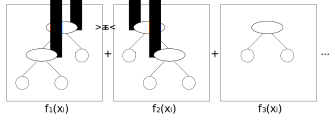
\includegraphics[scale=0.35]{figures/hmm/ensamble.pdf}}}
\caption{Figure (a) schematizes an individual decision tree, where in boolean splits based on the value of variables $v$ result in a categorization of signal or data as output. In a CART, the output is replaced by a continuous weight encoding ``signal-like'' versus ``background-like''. Figure (b) schematizes an ensemble of trees with different topologies, each defining an output function.}
\label{fig:}
\end{figure}

The information available for the training consists of datasets of $n$ entries and $m$ variables
The multi-dimensional entries $x_i$ $i\in[1,...,n]$ are labeled as either signal or background with $y_i$.
The elements of $x_i$ are variables $v_j$ $j\in[1,...,m]$.
The BDT is composed by of ensemble of decision trees.
A decision tree maps an entry of the dataset $x_i$ onto a discrete output space, such as a signal-vs-background likelihood.
Each node of the tree may represent a binary decision, or split, based on the variables of the entry.
Alternatively, the nodes with no children (leaves) may represent a decision, as illustrated in Figure \ref{fig:bdtTree}.
A generalization of a decision tree that assigns continuous weights to each leaf is a classification and regression tree (CART).
A tree can be \emph{trained} to map a set of input entries $x_i$ onto their corresponding labels $y_i$ by treating the distributions of input variables as PDFs and selecting splits (a, b, ...) that result in the highest output fidelity.
A single CART tends to struggle to represent the complexity of simulated physics datasets succinctly.
This performance can be augmented by an ensemble of CARTs labeled $k$, each with an output function $f_k(x_i)$ as illustrated in Figure \ref{fig:bdtTree}.
The output functions act as a \emph{model} of the provided dataset.
The sum of the CART output functions defines a new ensemble output function $f(x_i)=\hat{y}_i$, also called the discriminant score.

The training strategy is to develop an ensemble whose output functions accurately predict the corresponding label $y_i$ for unseen events.
This is quantified by a regularized loss function,
\begin{equation}\begin{split}\label{eqn:lossFunc}
    \mathcal{L}(\phi)=\sum_i l(\hat{y}_i,y_i),
\end{split}\end{equation} 
where $l$ measures the difference between $\hat{y}_i$ and $y_i$.
A process is defined to select trees, splits, and weights to minimize Equation \ref{eqn:lossFunc}.

The algorithm of \emph{boosting} is employed to minimize such loss functions by improving on the capability of a single CART.
It consists of iteratively expanding an ensemble of trees, with each addition addressing the mis-categorization of the previous ensemble.
One algorithm, \code{AdaBoost}, performs this task by iteratively reweighting poorly categorized entries to be more important to the following tree.
Another algorithm, \code{Gradient Boosting}, instead adds trees that are trained on the previous ensemble's poorly categorized entries.
Both of these algorithms played a role in the development of the analysis.
A descendent of \code{AdaBoost} and \code{Gradient Boosting} is \xgb, which introduces a modified loss function,
\begin{equation}\begin{split}\label{eqn:lossFuncXgb}
    \mathcal{L}(\phi)=\sum_i l(\hat{y}_i,y_i)+\sum_k \Omega(f_k).
\end{split}\end{equation} 
In Equation \ref{eqn:lossFuncXgb}, $\Omega$ is a measure of the complexity a tree.
The \xgb algorithm iteratively adds trees of diminishing weights, shrinking their importance by a constant factor.
It also introduces procedures to more quickly add and remove branches from trees while fitting the loss function.
These result in an accurate and reliable output function that can be trained quickly.
The \xgb algorithm was selected to construct the multivariate discriminant functions that are used in this analysis.
\cite{xgboost}

% Overtraining
It is a general goal to understand the underlying probability distributions that have produced a dataset, rather than of the dataset itself.
This applies to tasks such as training BDTs to discriminate signal from background, as well as fitting a functional form to data to model a background distribution. 
In both cases, the analytic model is interpreted as knowledge of these underlying distributions.
When solving an optimization problem such as those posed in Equations \ref{eqn:lossFunc} and \ref{eqn:lossFuncXgb}, the minimization algorithm has only the dataset at its disposal.
This can lead to \emph{over-training} or \emph{over-fitting}, where the optimization of the loss function tunes the discriminant to the features of a particular dataset rather than the features of the underlying distributions.
This problem tends to grow in step with the complexity of the model.
It is combatted, in part, by penalizing the optimization by the complexity of the model; the $\Omega$ function of Equation \ref{eqn:lossFuncXgb} is one such example.

Over-training may have two important and detrimental effects.
The first is to reduce the efficacy of the discriminant when applied to a new dataset.
Although this impacts the performance of the analysis, it does not necessarily invalidate the results by the introduction of bias.
The greater danger to the integrity of the analysis arises when the performance of the discriminant is inaccurately measured.
This second effect is illustrated in the following example.
Suppose a BDT is trained to identify signal events from a simulated dataset, and the same dataset is used to predict the number of signal events to expect in observed data.
A signal-rich category is defined based on the discriminant score for events.
In this case, simulated signal events tend to be over-represented in the category.
The BDT will identify simulated signal events with higher efficiency compared to signal in the data, leasing to an unconstrained uncertainty on the expected signal.
Unlike the first effect, this type of error invalidates the double use of the training simulation for further measurements.

\begin{figure}[h!]
\captionsetup[subfigure]{position=b}
\centering
\includegraphics[width=0.75\textwidth]{figures/hmm/testTrainVal.pdf}
\caption{The top row, $p_0$, shows an schematization of a dataset divided into five subsets with $k$-fold split with $k=5$.
The blue boxes represent sets to be used for training, the green boxes for validation, the red boxes for testing.
Five permutations of these assignments, $p_i$, are shown for the same dataset.
In cross-validation, a separate MVA is fit to each permutation, such that each entry of the full dataset belongs to the testing set for a particular MVA.
}
\label{fig:testTrainVal}
\end{figure}

The problem of over-training is mitigated by introducing a $k$-fold split of the available simulated datasets into a number, $k>2$, of subsets of similar multiplicity.
One subset is labeled as the ``testing'' set, and another is labeled as a ``validation'' set.
The remaining subsets are combined as a ``training'' set.
This is illustrated in the top of Figure \ref{fig:testTrainVal}.
The BDT algorithm is deployed on the training set, and further predictions with respect to the simulation are performed with the testing set.
Since the testing set has not been exposed to the BDT during training, there is no direct risk of over-training of the discriminant scores in the testing set.
There remains the issue of selecting thresholds that define the signal-rich category to optimize, for example, the expected sensitivity.
This choice is subject to the same concerns about over-training as the selection of trees during the training phase. 
A third set, the validation set, is defined orthogonally to both the training and testing sets.
This set is used to study the convergence of the training process, check for over-training effects that may reduce sensitivity, and, most importantly, to choose the discriminant thresholds for further categorization.

The final consideration is to inefficiency that such a division of the simulation set entails.
Simulated events are computationally expensive to produce.
A \emph{cross-validation} scheme calls for the permutation of each of the $k$ subdivisions, such that each event appears once in a test set, available for further analysis.
This is shown in Figure \ref{fig:testTrainVal}.
A separate BDT is trained with the training set from each permutation.
This means that each event in the full dataset has one discriminant score from a BDT for which it is in the testing set, one for which it is in the validation set, and $k-2$ for which it was in the training set.
The scores from the BDT for which an event was in the testing and validation sets are the testing and validation scores, respectively.

\subsection{Configuration}
\label{sec:hmmBdtConfiguration}

% Training details
Separate classifiers are trained for 3-lepton and 4-lepton categories, but there are many similarities between these.
A 5-fold splitting of the available signal and background simulation is used.
It is important to note that the testing set remains blinded until all choices related to the categorization channels have been fixed.
The output of the BDT on the testing set is final, and it is essential to refrain from making choices related to the procedure based on the testing set.
A cyclic permutation of the 5-fold splitting is used, such that a separate BDT is trained for each fifth of the total simulation.

% Samples
Each BDT is trained using the simulated background, in which all background components are included.
The signal for the 4-lepton BDTs are the qqZH samples, while the signal for the 3-lepton BDTs are the W$^\pm$H samples.
The per-event weights arising from scale factors and reweighing, along with the event corresponding to the campaign luminosity, cross-section, are provided to the BDT.
Negatively weighted events are removed, and the signal and background weights are both normalized.
% Sample statistics
The numbers of available simulated events for training are shown in table \ref{tab:hmmSampleStatistics}.

\begin{table}[htbp]
 \caption{Numbers of simulated events available for training, both in the full simulation, and the 3/5 training sets statistics.}
 \begin{center}
\begin{tabular}{l r r r}\toprule
Simulation           & Total Events & Training Events \\
\midrule
4-lepton signal      & 20700        & 12508    \\
4-lepton background  & 88314        & 53081    \\
3-lepton signal      & 134936       & 80962    \\
3-lepton background  & 185286       & 111107   \\
\bottomrule\end{tabular} 
 \end{center}
\label{tab:hmmSampleStatistics}
\end{table}

% Training variables
The set of variables provided as input for the BDT was chosen from a broader set of candidate variables with physical motivations.
This set was reduced in the order of ascending \emph{feature importance}, defined as the number of times the variable is used for a decision node, weighted by the number of events categorized by the node during training.
The reduction continued until the performance of the BDT began to decline.
Different variables are defined based on the different final state topologies in the inclusive 4-lepton and 3-lepton categories.
The variables for each are listed in Table \ref{tab:hmmVarNames}.

\begin{table}[htp]
\caption{Variable names and definitions used training the 3-lepton ($3\ell$) and 4-lepton ($4\ell$) BDTs. The second column indicates the BDT in which the variable was used, based on the lepton category number.}
\begin{center}
\begin{tabular}{l c l l}
\toprule
Variable & Used for BDT & Definition \\
\midrule
  $m_T(E_T^\text{miss},l1)$ & $3\ell$ & Transverse mass of the W candidate lepton and $E_T^\text{miss}$  \\
  $\Delta_\phi(E_T^\text{miss},H)$ & $3\ell$ & $\phi$ between $E_T^\text{miss}$ and the H candidate \\
  $E_T^\text{miss}$ & $3\ell$ & Missing transverse momentum \\
  $p_T^{l1}$ & $3\ell$ & W candidate lepton $p_T$ \\
  $\Delta_\phi(l1,H)$ & $3\ell$ & $\Delta$ $\phi$ between H candidate and W candidate lepton \\
  $\Delta_\eta(l1,H)$ & $3\ell$ & $\Delta$ $\eta$ between H candidate and W candidate lepton \\
  $p_T^{j1}$ & $3\ell$ and $4\ell$ & $p_T$ of leading jet (if present) \\
  $N_\text{jets}$ & $3\ell$ and $4\ell$ & Number of jets \\
  $p_T^{j2}$ & $4\ell$ & $p_T$ of subleading jet (if present) \\
  $\Delta_\phi(l1,l2)$ & $4\ell$ & $\Delta$ $\phi$ between the leptons paired for the Z candidate \\
  $\Delta_\phi(Z,H)$ & $4\ell$ & $\Delta$ $\phi$ between H candidate and Z candidate \\
  $\Delta_\eta(Z,H)$ & $4\ell$ & $\Delta$ $\eta$ between H candidate and Z candidate \\
  $m_Z$ & $4\ell$ & Z candidate mass \\
\bottomrule
\end{tabular}
\label{tab:hmmVarNames}
\end{center}
\end{table}


\afterpage{
\begin{figure}[h!]
\captionsetup[subfigure]{position=b}
\centering
\subfloat[][]{{\includegraphics[width=0.35\textwidth]{figures/hmm/public/kine/kine-3lep-aux1_met_mt.pdf}}}
\subfloat[][]{{\includegraphics[width=0.35\textwidth]{figures/hmm/public/kine/kine-3lep-aux1_pt.pdf}}}
\subfloat[][]{{\includegraphics[width=0.35\textwidth]{figures/hmm/public/kine/kine-3lep-aux1_uu_delta_eta.pdf}}} \\
\subfloat[][]{{\includegraphics[width=0.35\textwidth]{figures/hmm/public/kine/kine-3lep-aux1_uu_delta_phi.pdf}}}
\subfloat[][]{{\includegraphics[width=0.35\textwidth]{figures/hmm/public/kine/kine-3lep-j1_pt.pdf}}}
\subfloat[][]{{\includegraphics[width=0.35\textwidth]{figures/hmm/public/kine/kine-3lep-met_pt.pdf}}} \\
\subfloat[][]{{\includegraphics[width=0.35\textwidth]{figures/hmm/public/kine/kine-3lep-met_uu_delta_phi.pdf}}}
\subfloat[][]{{\includegraphics[width=0.35\textwidth]{figures/hmm/public/kine/kine-3lep-nJets.pdf}}}
\caption{Training variables provided as input for the for the 3-lepton classifier. The signal distribution shown in red is comprised of the simulated WH signal dataset, while the background distribution contains all background production modes shown in blue. Data distributions are included in black. Each distribution is normalized, and the error bars on each histogram are statistical only. }
\label{fig:hmm3lepVars}
\end{figure}
\clearpage
}

\afterpage{
\begin{figure}[h!]
\captionsetup[subfigure]{position=b}
\centering
\subfloat[][]{{\includegraphics[width=0.35\textwidth]{figures/hmm/public/kine/kine-4lep-auxDilep_delta_phi.pdf}}}
\subfloat[][]{{\includegraphics[width=0.35\textwidth]{figures/hmm/public/kine/kine-4lep-auxDilep_mass.pdf}}}
\subfloat[][]{{\includegraphics[width=0.35\textwidth]{figures/hmm/public/kine/kine-4lep-aux_uu_delta_eta.pdf}}} \\
\subfloat[][]{{\includegraphics[width=0.35\textwidth]{figures/hmm/public/kine/kine-4lep-aux_uu_delta_phi.pdf}}}
\subfloat[][]{{\includegraphics[width=0.35\textwidth]{figures/hmm/public/kine/kine-4lep-j1_pt.pdf}}}
\subfloat[][]{{\includegraphics[width=0.35\textwidth]{figures/hmm/public/kine/kine-4lep-j2_pt.pdf}}} \\
\subfloat[][]{{\includegraphics[width=0.35\textwidth]{figures/hmm/public/kine/kine-4lep-nJets.pdf}}}
\caption{Training variables provided as input for the for the 4-lepton classifier. The signal distribution shown in red is comprised of the simulated ZH signal dataset, while the background distribution contains all background production modes shown in blue. Data distributions are included in black. Each distribution is normalized, and the error bars on each histogram are statistical only. }
\label{fig:hmm4lepVars}
\end{figure}
\clearpage
}


%%%%%%%%%%%% Variable importance

% \begin{figure}[htpb]
%   \centering
%   \includegraphics[height=0.48\textwidth]{figures/hmm/nJets/histo-3lep-nJets.pdf}
%   \includegraphics[height=0.48\textwidth]{figures/hmm/zCand/histo-4lep-auxDilep_mass.pdf}
%   \caption{Left: N Jets distribution for 3-lepton channel, right: Z candidate mass for 4-lepton channel. These are the highest ranked in feature importance for their category's respective BDT's.}
%     \label{fig:hmmImpVars}
% \end{figure}

The feature importances for each training case are listed in Tables \ref{tab:3lepVarImport} and \ref{tab:4lepVarImport}.
In the 4-lepton case, the most important variable is the mass of the \Z candidate, which helps identify the signal.
In the 3-lepton case, the most important variable is the number of jets, which helps especially to separate out top quark backgrounds.

% \begin{figure}[htpb]
%   \centering
%   \includegraphics[height=8cm]{figures/hmm/bdtImportance/imp-4lep.pdf}
%   \includegraphics[height=8cm]{figures/hmm/bdtImportance/imp-3lep.pdf}
%   \caption{The 4-lepton (left) and 3-lepton (right) variables shown with their respective feature importance, averaged over the five BDTs trained for each cross-validation permutation. The importance of a variable is defined relative to the other variables.}
%     \label{fig:hmmVarImport}
% \end{figure}

\afterpage{
\begin{table}[htp]
\caption{Feature importance for the 3-lepton BDTs. The values shown are the feature importances normalized to the highest-importance variable. Values are given for individual BDTs along with a combined weight based on the sum across BDTs. The most important variable is the jet multiplicity.}
\begin{center}
\begin{tabular}{l ccccccc}
\toprule
Variable & BDT1 & BDT2 & BDT3 & BDT4 & Combined \\
\midrule
N Jets & 1.00 & 1.00 & 1.00 & 1.00 & 1.00 \\
$p_T^{j1}$ & 0.38 & 0.42 & 0.34 & 0.31 & 0.36 \\
$\Delta_\eta(l1,H)$ & 0.16 & 0.18 & 0.16 & 0.15 & 0.17 \\
$p_T^{l1}$ & 0.12 & 0.13 & 0.14 & 0.13 & 0.14 \\
$E_T^\text{miss}$  & 0.14 & 0.13 & 0.13 & 0.12 & 0.13 \\
$\Delta_\phi(E_T^\text{miss},H)$ & 0.09 & 0.08 & 0.10 & 0.10 & 0.09 \\
$m_T^{l1,E_T^\text{miss}}$ & 0.08 & 0.09 & 0.09 & 0.09 & 0.09 \\
$\Delta_\phi(l1,H)$ & 0.08 & 0.06 & 0.06 & 0.07 & 0.08 \\
\bottomrule
\end{tabular}
\label{tab:3lepVarImport}
\end{center}
\end{table}
%
\begin{table}[htp]
\caption{Feature importance for the 4-lepton BDTs, in the format of table \ref{tab:3lepVarImport}. The most important variable is the \Z candidate mass.}
\begin{center}
\begin{tabular}{l ccccccc}
\toprule
Variable & BDT1 & BDT2 & BDT3 & BDT4 & Combined \\
\midrule
$m_Z$ & 1.00 & 0.79 & 0.67 & 0.78 & 1.00 \\
N Jets & 0.99 & 1.00 & 1.00 & 1.00 & 0.89 \\
$p_T^{j1}$ & 0.78 & 0.44 & 0.19 & 0.25 & 0.60 \\
$\Delta_\eta(Z,H)$ & 0.45 & 0.39 & 0.37 & 0.51 & 0.55 \\
$p_T^{j2}$ & 0.12 & 0.41 & 0.49 & 0.58 & 0.31 \\
$\Delta_\phi(l1,l2)$ & 0.30 & 0.19 & 0.18 & 0.23 & 0.29 \\
$\Delta_\phi(Z,H)$ & 0.28 & 0.19 & 0.19 & 0.21 & 0.23 \\
\bottomrule
\end{tabular}
\label{tab:4lepVarImport}
\end{center}
\end{table}
\clearpage
}

The performance of a BDT is measured using the validation scores of the receiver operator curve (ROC).
The ROC is a parametric function of the BDT discriminant, plotted as the rate of correct signal categorizations (true positive rate) compared to the rate of false categorization of background as signal (false positive rate).
This is plotted in Figure \ref{fig:hmmBdtRoc} for a number of discriminant thresholds that define signal versus background.
A figure of merit used to evaluate the ROC is area-under-curve (AUC).
These show comparable performance for the BDTs of both categories and the impact of the relatively limited statistics of the 4-lepton sample.
As a cross check, the ROC curve for the training set is plotted along with the validation set. The agreement between these, within statistical uncertainty, does not indicate clear over-training effects.
The signal and background samples shown in the ROC plots correspond to the same samples used for the training; only WH and ZH signals are used in the definition of the ROC.

\begin{figure}[htpb]
  \centering
  \includegraphics[width=0.48\textwidth]{figures/hmm/bdtHist/roc-4lep-ZH-AllBackground-0-depth2-nEst80tag-new-AllBackground.pdf}
  \includegraphics[width=0.48\textwidth]{figures/hmm/bdtHist/roc-3lep-WH-AllBackground-0-depth2-nEst50tag-new-AllBackground.pdf}
  \caption{4 lepton (left) and 3 lepton (right) ROC curves for representative BDT's. Shown in black is the curve for the training set, while red shows the curve for the validation set (labeled test set). Error bars are statistical uncertainties due to the size of the training and validation datasets. The AUC is labeled on each plot.}
    \label{fig:hmmBdtRoc}
\end{figure}

% Figure \ref{fig:hmmBdtScoreLin} shows distributions of the BDT discriminant for different categories of signal and background, scaled the samples cross-section and luminosity.
% The signal/background separation is more apparent in this plot than in those normalized to the physical expectation.


% \begin{figure}[htpb]
%   \centering
%   \includegraphics[width=0.48\textwidth]{figures/hmm/bdtHist/bar20-4lep-ZH-AllBackground-0-depth2-nEst80tag-new-AllBackground.pdf}
%   \includegraphics[width=0.48\textwidth]{figures/hmm/bdtHist/bar20-3lep-WH-AllBackground-0-depth2-nEst50tag-new-AllBackground.pdf}
%   \caption{4 lepton (left) and 3 lepton (right) distributions of the BDT discriminant, where the signal and background samples share a normalization. The signal distribution is that of the sample used for training, not the full signal MC sample.}
%     \label{fig:hmmBdtScoreLin}
% \end{figure}

Figure \ref{fig:hmmBdtScore} shows the BDT discriminant calculated in different categories and scaled by the samples cross-section and luminosity.
The signal and background composition is more apparent in these plots: primarily, the target signal production mechanism is separated from other signals.
The top backgrounds are particularly well separated owing in part to the high statistics available for these samples in the training sets.

% {\color{red} This paragraph section is slightly redundant. Merge into next section?}
% Exclusive categories are defined based on discriminant cuts that produce varying levels of signal purity.
% The category ``4-lepton high-purity'' is defined in the 4-lepton selection by requiring 4-lepton BDT score greater than 0.12. 
% Two categories are defined from the 3-lepton selection: ``3-lepton high-purity'' and ``3-lepton middle-purity''. 
% The former is selected by requiring 3-lepton BDT score greater than 0.7,
% and the latter is selected by requiring 3-lepton BDT score less than 0.7
% but greater than 0.1.
% The events failing VH categorization are still considered in the inclusive categories.
 
\begin{figure}[htpb]
  \centering
  \includegraphics[width=0.48\textwidth]{figures/hmm/public/bdt/histo-4lep-bdtScore.pdf}
  \includegraphics[width=0.48\textwidth]{figures/hmm/public/bdt/histo-3lep-bdtScore.pdf}
  \caption{4-lepton (left) and 3-lepton (right) distributions of the BDT discriminant, using the final test scores. The simulated background is shown in shaded grey, while the signal distributions are drawn as lines in red for ZH and orange for WH. The remaining non-VH production mechanisms (ggF, VBF, and ttH) are combined and plotted as a dark grey line. All the signal histograms have been scaled by a factor of 50 to enhance visibility.\\
  It is observed that the score separates the signal to the left and background to the right. Of similar importance is that it specifically isolates the VH signal of interest and not the other signal productions. For 4-lepton this is the ZH signal and for 3-lepton this is the WH signal. Vertical dotted lines indicate the values that delineate which events belong in which final categories. The full dataset is included as well, which is used to fix the normalization of the background. \\
  The 3-lepton discriminant separates signal from background to a higher degree than does the 4-lepton discriminant. This is due in part to the stricter 4-lepton event selection, which can remove many more ``easily'' separable background events. The remaining events are more similar, topologically, to the ZH signal.}
    \label{fig:hmmBdtScore}
\end{figure}

\subsection{Categorization}

The event selection results in two inclusive categories distinguished by lepton number: the 4-lepton and 3-lepton categories.
These selections are further divided into \emph{exclusive} categories based on the relative purity of the signal.
This subsequent division is based on the BDT discriminant scores for each event.
The 4-lepton category is divided once into low-purity and high-purity categories.
The 3-lepton category, with a greater event multiplicity, is divided into low-, medium-, and high-purity categories.

Each event belongs to both a validation dataset and a testing dataset, each of which has an associated discriminant score.
The validation scores are considered when selecting the score thresholds delineating categories.
The testing scores are used for the final hypothesis test and limit setting.
An optimization scan over various thresholds of the expected significance determines the threshold values.
The thresholds are selected in order to produce the highest expected significance, based on the validation scores.
These thresholds are specified in Table \ref{tab:hmmBdtCuts}.

\begin{table}[htp]
\caption{Category definitions based on the ranges of the discriminant value $O$. The output of the BDT is scaled such that $O\in[0,1]$, with higher numbers corresponding to VH-like events.}
\begin{center}
\begin{tabular}{c c c l l l}
\toprule
Inclusive Category & Exclusive Category & Criteria \\
\midrule
\multirow{2}{*}{4-Lepton} & High-purity & $O\ge0.12$ \\
                          & Low-purity & $O<0.12$ \\
\midrule
\multirow{3}{*}{3-Lepton} & High-purity & $O\ge0.72$ \\
                          & Middle-purity & $0.10\ge O<0.72$ \\
                          & Low-purity & $O<0.10$ \\
\bottomrule
\end{tabular}
\label{tab:hmmBdtCuts}
\end{center}
\end{table}

To first choose the thresholds using the testing set and then perform a hypothesis test in categories defined by that threshold would lead to a misleading signal and background expectation in those categories.
The choice of threshold would be biased to the statistical fluctuations in the test dataset.
This results in categories biased to contain more simulated signal events and fewer simulated background events than would be expected in the data.
Since the analysis of the data includes the signal model based on simulation, such a method is unacceptable.

\begin{figure}[htpb]
  \centering
  \includegraphics[width=0.45\textwidth]{figures/hmm/public/postCut/histo-4lep0-muu.pdf} \\
  \includegraphics[width=0.45\textwidth]{figures/hmm/public/postCut/histo-3lep0-muu.pdf} 
  \includegraphics[width=0.45\textwidth]{figures/hmm/public/postCut/histo-3lep1-muu.pdf} 
\caption{Distributions of \muu in the 4-lepton (top) and 3-lepton (bottom) selections after categorization based on a cut on the BDT discriminant score.}
    \label{fig:hmmPostcutMassHists}
\end{figure}
\clearpage

The high and middle-purity categories are considered for further analysis.
The low-purity events, containing few expected signal events, are only analyzed in the inclusive categories defined prior to BDT cut.
The distributions of \muu are shown in Figures \ref{fig:hmmPrecutMassHists} and \ref{fig:hmmPostcutMassHists}.
The former shows the inclusive distribution before further categorization with the BDT discriminant.
The latter shows the distributions in the categories defined in Table \ref{tab:hmmBdtCuts}.
The motivation to use the discriminant becomes apparent in these plots when compared to Figure \ref{fig:hmmPrecutMassHists}.
In both the 4-lepton and 3-lepton high-purity categories, Drell-Yan production has been virtually removed.
The background remaining is primarily from diboson sources.
The signal selection purity is also evident in the high-purity categories: these produce homogeneous selections of events from ZH or WH productions, depending on their target.


\input{sections/hmumu-bkg}
\section{Signal Modeling}\label{sec:hmmSig}

This section describes the signal contribution to the various categories defined in Section \ref{sec:hmmBdt}.
The expected signal contribution in each category is modeled in the \muu distribution with the simulated datasets described in Section \ref{sec:hmmSim}.
As the production mechanism is essentially indistinguishable in terms of signal shape, no further effort is made to separate events originating from VH mechanisms from ggF, VBF, or ttH mechanisms.
From this point, the ensemble of production mechanisms is combined and referred to as \emph{signal}.

An empirical functional form is used to parameterize the shape of the signal distribution.
The natural width of the Higgs decay ($\Gamma_\text{H}\approx4$~MeV) is too small to resolve at ATLAS.
The signal shape is consequently determined by the momentum resolution for muons.
As such, a reasonable choice of function is the double sided Crystal Ball (CB) given in Equation \ref{eq:hmmSignal}.
\begin{equation}\label{eq:hmmSignal}
  f_\text{S}(m_{\mu\mu}) =
  \begin{cases}
  \text{CB}_\text{high}(\alpha_\text{high},n_\text{high},\sigma,\bar{x}) & \text{for }m_{\mu\mu}>\bar{x}\\
  \text{CB}_\text{low}(\alpha_\text{low},n_\text{low},\sigma,\bar{x}) & \text{for }m_{\mu\mu}<=\bar{x}\\
  \end{cases}
\end{equation}
Here, $\alpha_\text{low}$ and $\alpha_\text{high}$ values are the cross-over value for the high and low CB functions.
The other parameters are the shared mean and width of the CB functions, $\bar{x}$ and $\sigma$,
while $n_\text{low}$ and $n_\text{high}$ are the powers for the power-law tails of the high and low CB functions.
The CB function itself is defined in Equation \ref{eqn:hmmCb}.
\begin{equation}\label{eqn:hmmCb}
    \text{CB}(x,\alpha,n,\bar{x},\sigma) = 
    \begin{cases}
        \exp{-\frac{(x-\bar{x})^2}{2\sigma^2}} & \text{for }\frac{(x-\bar{x})}{2\sigma}>-\alpha \\
        \left(\frac{n}{|\alpha|}\right)^n \exp{-\frac{|\alpha|}{2}} \left(\frac{n}{|\alpha|}-|\alpha|\right)^{-n} & \text{otherwise}\\
    \end{cases}
\end{equation}
The CB function is normalized when treated as a PDF.
In the signal model, the normalization is scaled to match the expected number of signal events.

The following diagrams in Figure \ref{fig:hmmSignalFit} show fits of the signal model to the simulated distribution, both before and after categorization with the BDT score.
The corresponding fitted values of signal model parameters parameters are listed in Table \ref{tab:hmmSignalFit}.



\afterpage{
\begin{minipage}{\textwidth}
\begin{figure}[H]
  \centering
  \subfloat[][]{{\includegraphics[width=0.30\textwidth]{figures/hmm/signalFits2/sigfit-3lep.pdf}}}
  \subfloat[][]{{\includegraphics[width=0.30\textwidth]{figures/hmm/signalFits2/sigfit-4lep.pdf}}}\\
  \subfloat[][]{{\includegraphics[width=0.30\textwidth]{figures/hmm/signalFits2/sigfit-3lep0.pdf}}}
  \subfloat[][]{{\includegraphics[width=0.30\textwidth]{figures/hmm/signalFits2/sigfit-4lep0.pdf}}}
  \subfloat[][]{{\includegraphics[width=0.30\textwidth]{figures/hmm/signalFits2/sigfit-3lep1.pdf}}}
  \caption{Fits of the signal model to the simulated signal in each categories. 
On top, (a) shows 3-lepton and (b) shows 4-lepton inclusive categories.
Below, (c and d) show 3-lepton HP and MP, and (e) shows 4-lepton LP.
The blue line shows the fitted signal function, while the black dots show the simulation with statistical errors.
}
    \label{fig:hmmSignalFit}
\end{figure}
% #
% \vspace{-2em}
\begin{table}[H]
 \caption{Parameters of the signal model fit to simulation.}
 \begin{center}
\begin{tabular}{l r r r r r}\toprule
Parameter & 4-lepton & 3-lepton & 4-lepton HP & 3-lepton LP & 3-lepton HP \\
\midrule
$\alpha_\text{low}$ & 1.11 & 1.32 & 1.15 & 1.36 & 1.33 \\
$n_\text{high}$ & 15.65 & 26.93 & 13.68 & 23.92 & 58.46 \\
$\bar{x}$ & 124.5 & 124.5 & 124.4 & 124.5 & 124.5 \\
$\alpha_\text{high}$ & 1.43 & 1.48 & 1.51 & 1.50 & 1.41 \\
$\sigma$ & 2.79 & 2.91 & 2.84 & 2.88 & 2.92 \\
$n_\text{low}$ & 4.59 & 2.67 & 4.94 & 2.04 & 2.94 \\
\bottomrule\end{tabular}
 \end{center}
\label{tab:hmmSignalFit}
\end{table}
\end{minipage}
\clearpage
}


\subsection{Signal+Background Model}

It is helpful to define the predictions of various ``signal+background'' (S+B) hypotheses.
This combines the signal prediction from Equation \ref{eq:hmmSignal} with the background prediction in Equation \ref{eqn:hmmBkgFunc}.
The Standard Model predicts a particular signal multiplicity, $N_{SM}$.
The relative amplitude of the signal compared to the prediction of the Standard Model is defined as the \emph{signal strength}, \mus.
A range of S+B hypotheses are possible, labeled by the signal strength.
For example, \mus=1 describes a hypothesis with the Standard Model signal strength, while \mus=0 describes a ``background-only'' (B) hypothesis.

The S+B hypothesis predicts the relative frequency of events as a function of \muu.
It is defined in Equation \ref{eqn:hmmSbFunc} as the sum of the normalized signal shape PDF $f_\text{S}(\muu)$, and the normalized background PDF $f_\text{B}(\muu)$.
\begin{equation}\begin{split}\label{eqn:hmmSbFunc}
f_\text{S+B}(\muu) = N_\text{S}\times f_\text{S}(\muu) + N_\text{B}\times f_\text{B}(\muu)
\end{split}\end{equation} 
There are three free parameters in Equation \ref{eqn:hmmSbFunc}: the shape parameters $a$ and $b$ that describe the background, and $N_\text{S}\equiv\mus\times N_{SM}$ where \mus is free.
Each of these may be adjusted by \code{minuit} to fit the data distribution in each category.
The overall normalization of the function, when treated as a PDF, is normalized as was the case with the background-only function.

In the case that a strong signal is not observed in the data, it is still possible to consider which S+B hypotheses are compatible and incompatible with the observation.
In this case, some set of hypotheses are considered excluded to a particular confidence level.
To this end, an S+B hypothesis is defined by a fixed \mus, and free parameters $a$ and $b$.

\input{sections/hmumu-systematics}
\input{sections/hmumu-statistics}

\section{Results}\label{sec:hmmResults}
\subsection{Significance}

The observed data is fit with the B-only and S+B models.
The event multiplicity in the invariant-mass range $\muu\in[120,130]$~GeV is of principle interest, as this region contains the majority of the VH produced events.
The observed yields are provided in Table \ref{tab:hmmResultNdat}.
The number of expected background events, based on the B-only model fit in the invariant-mass sidebands $\muu\in[110,120]\cup[130,160]$, is listed as well.
The first observation is of the excesses of observed events over the expected events in the inclusive 4-lepton and 3-lepton categories.
These excesses are preserved in the post-cut exclusive categories, with a particular excess in the 4-lepton high purity category.
It is interesting to note that the subsequent measurement by CMS found a similar excess in leptonic VH events\cite{cmsHmm}. 

\begin{table}[htp]
\caption{
Yields of data and expected background counted in invariant-mass range $\muu\in[120,130]$~GeV, corresponding to 139 fb$^{-1}$ of integrated luminosity.
The uncertainties on the background estimate are described in Section \ref{sec:hmmBkgUncert}.
}
\begin{center}
\begin{tabular}{l r r r r r}\toprule
Category               & Data    & Background \\
\midrule
4-Lepton               & 51      & 44.5$\pm$2.7 \\
3-Lepton               & 437     & 402.3$\pm$21.0 \\
\midrule
4-Lepton High-Purity   & 34      & 19.1$\pm$1.5 \\
3-Lepton High-Purity   & 41      & 34.2$\pm$2.3 \\
3-Lepton Middle-Purity & 358     & 329.7$\pm$18.7 \\
\bottomrule\end{tabular}\\
\label{tab:hmmResultNdat}
\end{center}
\end{table}

The significances of these observations under the background-only hypothesis are given in Table \ref{tab:hmmSignificance}.
The top of the table shows these for the inclusive categories, while the bottom shows values for the exclusive categories.
The exclusive and inclusive significance are separated to emphasize that these observations are correlated.
Also listed are the probabilities (p-values) to observe a result more incompatible than the observation, supposing the background-only hypothesis.
The p-values are calculated with a frequentist approach. 
An ensemble of 100,000 statistical toys are used to estimate the likelihood of observations under the background-only hypothesis with ensembles of statistical toys.

\begin{table}[htp]
\caption{Significance and p-values of the observed data yield in $\muu\in[120,130]$~GeV given the expected background.}
\begin{center}
\begin{tabular}{l r r r r r}\toprule
Category & Significance $\sigma$ & p-value \\
\midrule
3-Lepton & 0.75 & 0.23 \\
4-Lepton & 0.70 & 0.24 \\
\midrule
4-Lepton High Purity & 2.47 & 0.01 \\
3-Lepton High Purity & 0.83 & 0.20 \\
3-Lepton Middle Purity & 0.69 & 0.25 \\
\bottomrule\end{tabular} %remember cline{1-2}
\label{tab:hmmSignificance}
\end{center}
\end{table}

The largest significance is that of the observation in the 4-lepton High-Purity category, approaching 2.5$\sigma$.
The combined significance of observations in the inclusive 4-lepton and 3-lepton categories is $1.03\sigma$.
As a result of the higher sensitivity of the exclusive categories, the exclusive observations have a combined significance of $2.70\sigma$.
These observations can be compared to two similar observations.
First, the CMS collaboration has reported a significance in their leptonic VH \hmm observation with a significance of 2.02$\sigma$ \cite{cmsHmm}.
Other observations by the ATLAS experiment have been made for VH production in different Higgs boson decay channels: $\gamma\gamma$, $\Z\Z$, and $b\bbar$.
These previous observations all report a modest excesses of events that is compatible at a level of $\approx1\sigma$ with the Standard Model prediction \cite{atlashiggs}.


\subsection{Limits}

The observed invariant-mass distributions are shown in Figures \ref{fig:hmmFits}.
The S+B model (Equation \ref{eqn:hmmSbFunc}) and B-only (Equation \ref{eqn:hmmBkgFunc}) models, fit to the data, are shown.
The excesses of events shown in Table \ref{tab:hmmResultNdat} results in positive measurements of the signal strength, \mus, in each category.


\afterpage{
\begin{figure}[htp]
\captionsetup[subfigure]{position=b}
\centering
\includegraphics[width=0.45\textwidth]{figures/hmm/fitData2/ratio-4lep-dat.pdf}
\includegraphics[width=0.45\textwidth]{figures/hmm/fitData2/ratio-3lep-dat.pdf}\\
\includegraphics[width=0.45\textwidth]{figures/hmm/fitData2/ratio-3lep0-dat.pdf}
\includegraphics[width=0.45\textwidth]{figures/hmm/fitData2/ratio-3lep1-dat.pdf}\\
\includegraphics[width=0.45\textwidth]{figures/hmm/fitData2/ratio-4lep0-dat.pdf}
\caption{The S+B (red) and B-only (blue) models fit to data (black).}
\label{fig:hmmFits}
\end{figure}
\clearpage
}


% \begin{figure}[htp]
% \captionsetup[subfigure]{position=b}
% \centering
% \subfloat[][]{{\includegraphics[width=0.5\textwidth]{figures/hmm/fitData2/ratio-4lep-dat.pdf}}}
% \subfloat[][]{{\includegraphics[width=0.5\textwidth]{figures/hmm/fitData2/ratio-3lep-dat.pdf}}}
% \caption{Fits of the S+B and B-only models to the data observed in the inclusive 4-lepton (a) and 3-lepton (b) categories.}
% \label{fig:hmmPrecutFits}
% \end{figure}

% \begin{figure}[htp]
% \captionsetup[subfigure]{position=b}
% \centering
% \subfloat[][]{{\includegraphics[width=0.5\textwidth]{figures/hmm/fitData2/ratio-4lep0-dat.pdf}}}\\
% \subfloat[][]{{\includegraphics[width=0.5\textwidth]{figures/hmm/fitData2/ratio-3lep0-dat.pdf}}}
% \subfloat[][]{{\includegraphics[width=0.5\textwidth]{figures/hmm/fitData2/ratio-3lep1-dat.pdf}}}
% \caption{Fits of the S+B and B-only models to the data observed in the exclusive 4-lepton high-purity (a), 3-lepton high-purity (b), and 3-lepton middle-purity categories.}
% \label{fig:hmmPostcutFits}
% \end{figure}

% \begin{table}[htp]
% \caption{Asymptotic upper limits set at 95\% confidence levels on the signal strength \mus in each of the inclusive (top) and exclusive (bottom) categories. The signal strength corresponds to a number of signal events $N_S$, and these are provided as well.}
% \begin{center}
% \begin{tabular}{l r r r r r }
% \toprule
% \multirow{2}{*}{Category} & \multicolumn{2}{c}{Limit on $N_S$} & & \multicolumn{2}{c}{Limit on \mus} \\
% \cline{2-3} \cline{5-6} 
% & Expected & Observed & & Expected & Observed \\
% \midrule
% 3-Lepton & 63.7 & 112.5 & &  13.2 & 22.6 \\
% 4-Lepton & 23.2 & 30.1 & &  33.2 & 42.8 \\
% \midrule
% 4-Lepton High-Purity & 14.7 & 28.3 & &  23.7 & 45.1 \\
% 3-Lepton Middle-Purity & 58.1 & 94.4 & &  18.7 & 29.8 \\
% 3-Lepton High-Purity & 20.6 & 29.5 & &  12.0 & 17.2 \\
% \bottomrule
% \end{tabular}
% \label{tab:hmmLimits}
% \end{center}
% \end{table}


The observed data shown in these figures restrict the plausibility of signal production mechanisms that predict events produced in the range $\muu\in[110,160]$.
Exclusion limits are set on the largest signal mechanisms that retain compatibility with the data.
The Standard Model VH \hmm production, scaled by a coefficient \mus, is used as a set of benchmark signal models for this purpose.
These limits are set in the fiducial volume defined in Section \ref{sec:hmmEv}, in the invariant-mass range $\muu\in[110,160]$.
They apply to the production of Higgs-like signal events in the inclusive and exclusive categories.

\begin{table}[H]
\caption{Upper limits set at 95\% confidence levels on the signal strength \mus in each of the inclusive (top) and exclusive (bottom) categories. The signal strength corresponds to a number of signal events $N_S$, and these are provided as well. These frequentist limits are set with $\approx$ 50,000 toys.}
\begin{center}
\begin{tabular}{l r r r r r }
\toprule
\multirow{2}{*}{Category} & \multicolumn{2}{c}{Upper limit on \nsig} & & \multicolumn{2}{c}{Upper limit on \mus} \\
\cline{2-3} \cline{5-6} 
& Expected & Observed & & Expected & Observed \\
\midrule
3-Lepton & 52.9 & 110.3 & & 10.7 & 22.2 \\
4-Lepton & 17.1 & 30.1 & & 24.3 & 42.6 \\
\midrule
4-Lepton High Purity & 12.7 & 29.0 & & 20.3 & 46.1 \\
3-Lepton High Purity & 16.0 & 29.7 & & 9.3 & 17.3 \\
3-Lepton Middle Purity & 47.0 & 92.4 & & 14.9 & 29.2 \\
\bottomrule
\end{tabular}
\label{tab:hmmLimits}
\end{center}
\end{table}

% inclusive
The top half of Table \ref{tab:hmmLimits} reports limits set at 95\% confidence level in the inclusive categories.
The fiducial volumes for the inclusive categories specify a multi-lepton phase space but do not detailed further requirements on the kinematic character of a potential signal.
This makes these limits relatively model-independent and interpretable in terms of other signal production mechanisms.
For this purpose, the limits are provided both on the signal strength \mus for the Standard Model VH, and in terms of the number of signal events, \nsig.

% exclusive
The bottom half of the Table \ref{tab:hmmLimits} presents limits set in the exclusive categories.
The use of the MVA discriminant in the case of the exclusive categories means that these limits are only applicable to signal models with the same kinematic distributions as the Standard Model Higgs. 
For these, the limits on the Standard Model signal strength are most relevant.

The limits on the \nsig are equivalent to limits on the visible cross-section times branching ratio, \xsbr, times the dataset luminosity.
In all cases, the excesses reported in Table \ref{tab:hmmResultNdat} result in weaker observed limits than expected.
The particularly large excess observed in the 4-lepton high purity category raises the observed limit to over twice the expected limit.

\subsection{Other production mechanisms}

The observations made in the three exclusive VH categories are included in a combined search for \hmm that includes categories targeting additional production mechanisms.
In particular, a superset of the VH event selection identifies events with at least dimuon pair.
Events with a b-jet are identified as ttH candidates.
Events with two jets and a kinematic profile that matches simulated VBF production are identified as VBF candidates.
The remaining events are ggH candidates and are separated into zero, one, and two jet categories.
Each category is separated into four sub-categories using an MVA discriminant.
The composition and purity of these categories are illustrated in Figure \ref{fig:hmmComb}.
\cite{atlasHmm}

The combined categories are used to set limits at 95\% confidence on the Standard Model production of \hmm events.
The observed (expected) limit is 2.0 (1.7) times the Standard Model cross-section times branching ratio, reflecting an overall excess of observed events over the background prediction in the signal region.
This provides a strong hint of the \hmm production at the LHC.

\afterpage{
\begin{figure}[h!]
\captionsetup[subfigure]{position=b}
\centering
\includegraphics[width=0.99\textwidth]{figures/hmm/comb/Categorisation_.pdf}
\caption{
Overview of the signal and background compositions in the twenty analysis categories used in the combined \hmm search.
The VH categories are indicated in bold text.
Each quantity is calculated in $\mh\in[120,130]$~GeV based on simulation.
(Top) Ratios of signal to background yields. 
(Middle) Relative signal compositions.
(Bottom) Relative background compositions.
}
\label{fig:hmmComb}
\end{figure}
\clearpage
}

\subsection{Summary}

This chapter presented a search for the rare decay of the Standard Model Higgs boson to two muons using the VH production channels.
This search is challenging on two accounts.
First, tiny branching fraction of the Higgs boson to muons limits the production of events from such production mechanisms.
Second, the large irreducible background of dimuon events serves to mask the rare signal events.
A new strategy is adopted to use the leptonic final state of VH production.
The additional leptons in the final state are used to separate VH events from the Drell-Yan, diboson, and top backgrounds.
This particular phase space previously had not been investigated by either the ATLAS or CMS collaborations.

Identifying events from \vhmm production is complicated by the small leptonic branching ratio of the \W and \Z bosons.
However, making use of the additional kinematic information from the leptons yields a powerful lever to further reduce backgrounds.
% Techniques to address challenge
A new set of selection criteria captures as many VH events as possible.
Machine-learning methods in the form of a multivariate analysis discriminant are used to take advantage of the kinematic information from the W/Z decays.
Careful use of k-fold splitting and test/validation/train designations are introduced to avoid introducing uncontrolled bias.

Moderate excesses are seen above the expected number of events in the three and four lepton categories.
In the inclusive categories the observations remain compatible with the background-only hypothesis.
The combined significance of the inclusive observations is 1.03$\sigma$.
In the more sensitive exclusive categories, tension is observed in the 4-lepton high purity category and not in the others.
% No significant departure from the expected background is observed in data.
Limits are set on VH Higgs-like signal hypotheses.
The strongest expected (observed) limit on leptonic VH production excludes signals down to 10.8 (22.3) times the Standard Model prediction.
These limits are the first to be set in this particular phase space.
Limits are set on the numbers of signal events in 3-lepton and 4-lepton fiducial volumes.
These exclude the visible cross-section times branching ratio those regions above \xsbr=0.39~fb and \xsbr=0.22~fb, respectively.


\chapter{Search for Non-resonant Signatures and Contact Interactions}\label{sec:ci}

% Physical processes that produce a pair of final state leptons offer a clear window into the dynamics of high energy collisions.
Observations of pairs of leptons, both of electron and muon flavors, offer a clear window into the dynamics of high energy collisions.
The clarity of this window is due to the long lifetime and ease of detection offered by those leptons.
Of particular use is the invariant-mass spectra of dilepton pairs, which elucidates the possible mechanisms of their production by means of local enhancements, or resonances. 
This has proved a useful tool that has been exploited throughout the history of experimental particle physics.
In 1974, a group working at Brookhaven National Laboratory\cite{jpsiBnl} and another group working at the Stanford Linear Accelerator Center\cite{jpsiSlac} used the dielectron mass spectrum to independently discover the \jpsi resonance at \mee=3.1~GeV.
In 1977, a group working at Fermilab used the dimuon mass spectrum to discover the $\Upsilon$ resonance at \muu=9.5~GeV \cite{upsilon}.
In 1983, the UA1 group working at the SPS collider at CERN used both dielectron and dimuon events to detect the decay of the \Z boson at a mass of $\mll\approx95$~GeV\cite{z0ua1}.
Later in the same year, the UA2 group used dielectron events to produce a measurement of \mee=91.9~GeV.
The utility of the dilepton final state is derived from the fact that the final state consisting of two leptons is fully reconstructible.

\begin{figure}[htp]
\captionsetup[subfigure]{position=b}
\centering
\includegraphics[width=0.7\textwidth]{figures/ci/lowmass/lowmass-lower.pdf}
\caption{The invariant-mass spectra around the \Z boson mass peak from one million collisions with two muons.}
\label{fig:ciLowMass}
\end{figure}

% General non-resonant
The discoveries made with the invariant-mass spectra associate enhancement in rate of observed events with new mechanisms responsible for the enhancement.
These enhancements may be localized, as is the case for narrow resonances produced by \jpsi decay.
Alternatively, broad enhancements are possible as well; such enhancements, termed \emph{non-resonant}, are the focus of this search.
\footnote{Broad deficits are possible as well; one example is the observations of negative (positive) interference between $\gamma^*$ and \Z that changes the forward-backward charge symmetry below (above) the \Z mass peak in electron-positron experiments \cite{fbasym}.}
The investigation presented in this chapter contemplates the dielectron and dimuon invariant mass spectra in search for new and broad excesses appearing in the high mass tail.

Many new physics models beyond the Standard Model predict broad enhancements in dilepton production.
% Contact interactions
A particularly interesting cause of a non-resonant signature is a \emph{contact interaction} (CI) between quarks and leptons at an energy scale exceeding that of the collision energy.
Although direct resonant production is inaccessible, a new contact interaction would lead to off-shell production and interference with the SM production.
This can be caused by a mediator particle with a mass far above the \sqrts=13~TeV collision energies offered by the LHC.
A \qqll CI is also interesting because it is a necessary outcome of quarks and leptons sharing a common substructure \cite{eichten}.

Many new physics models outside the Standard Model predict non-resonant excesses.
To maintain a degree of generality and model independence, the products of this search are designed to be agnostic as to the underlying mechanism behind the feature.
As a result, when possible, the procedure used to produce results tends to limit or exclude the role played by signal models.
Due to the nature of the chosen analysis strategy, several choices must be made with respect to the region of date in which the search is conducted.
In these cases, the analysis is designed in order to optimize sensitivity to a generic formulation of contact interaction that serves as a benchmark.
This model dependant optimization remains, for the greater part, separate from the final results.

\begin{figure}[h!]
\captionsetup[subfigure]{position=b}
\centering
\includegraphics[width=0.99\textwidth]{figures/ci/massRanges.pdf}
\caption{
A schematic example of the dilepton invariant mass spectrum. 
The monotonically falling total background shape is shown by the solid black line, while the dotted red line shows an example of a CI signal plus the total background shape.
A background model is fit to the data it in a low-mass control region (shaded blue area) where a potential bias from the presence of a signal is negligible.
The resulting background shape is extrapolated from the control region into the high-mass signal region (shaded red area).
% The gap illustrated between the CR and the SR is found to be the preferred case for the destructive interference cases only.
}
\label{fig:ciStrat}
\end{figure}

% Challenges
This search for contact interactions is carried out using the dielectron and dimuon invariant-mass spectra.
Since CI produce final states of the same topology as some SM backgrounds, the signal production interferes either constructively or destructively with these backgrounds.
In the constructive case, the CI strictly enhances the spectra with a broad non-resonant shape.
In the destructive case, the interference modifies the background spectra as illustrated in Figure \ref{fig:ciStrat}. 
Both types of interference are considered in this analysis.

This search is complicated by both experimental and phenomenological challenges.
It involves probing the highest energy regimes and smallest length scales ever accessed by observation.
The first challenge results from the width of the non-resonant shape of interest, as shown in the red line of Figure \ref{fig:ciStrat}.
This shape is qualitatively similar to the shape of the background, so care must be taken to avoid interpreting an existing signal as background, thereby losing sensitivity to new physics.
The second challenge is the focus on new CI signals that may manifest themselves in the tail of the invariant-mass spectra.
Attention must be paid to systematic uncertainties in this regime, as well as to the relevant resolution of the measured spectra.
The third challenge is in modeling statistical knowledge of the background in signal regions with very low occupancy.
The sensitivity of the analysis is similarly impacted by statistical and experimental uncertainties on the background expectation, as these are of similar magnitude of the background itself.
New techniques are required to properly address these challenges.

% new analysis strategy: data-driven
This analysis introduces a number of changes that depart from previous searches.
The result presented here is the first non-resonant dilepton search at the LHC to use a functional form fit to data to estimate the background, rather than a background estimate derived from simulated events.
This choice removes the dependence of the background on the theoretical assumptions involved in the simulation process.
This is important because these assumptions are both significant and poorly constrained in the high-mass regime.

% Solution: avoid fitting signal shape
The contact interactions that provide a benchmark model predict deviations from the expected gradient of the high-mass tail of the dilepton mass spectrum; the subtlety of this effect could easily be masked by a background description of sufficient flexibility to match the data.
Therefore, the background event distribution at high masses is estimated based on a low-mass control region (CR) where the contribution of the benchmark signals are negligible.
A functional form is fit to the observed data in the CR, and extrapolated to higher masses to model the production rate of background events.
The search is then performed in a high-mass signal region (SR); here, event production by the benchmark signals is predicted to dominate over the background production.
The arrangement of these mass ranges is illustrated in Figure \ref{fig:ciStrat}.
The extrapolation from CR to SR avoids fitting the data in the regime where CI signals could potentially perturb the fit.
This strategy reduces the impact of a signal shape, if present in the data, on the fitted background model.

% Solution: avoid resolution, etc
ATLAS measures electron transverse energy, \et, and muon transverse momentum, \pt.
Consequently the invariant-mass resolution of dielectron pairs depends on \et resolution.
For high-\et electrons, this grows as a constant fraction of \et. 
Meanwhile, the invariant-mass resolution of dimuon pairs depends on \pt.
As a result, the fractional muon resolution grows linearly with \pt.
Both of these resolutions propagate to their respective invariant-mass spectra.
A single-bin SR is used to combat the effects of these resolutions, which are particularly impactful in the high-mass regime.
All events falling within the SR are counted identically, which mitigates the importance of \et and \pt resolution.
This approach has the additional benefit of removing shape information in the signal region, making the results readily reinterpretable for signal models predicting different non-resonant shapes.

% new analysis strategy: Bayesian
A key part of this analysis is the statistical treatment of the observations.
The Bayesian statistics used in previous ATLAS and CMS searches for CI has been replaced frequentist statistical framework.
This removes the dependence of the result on prior probabilities to observe a signal.
If the interference between signal and SM processes is not negligible, as is the case for CI, the choice of one prior over another is poorly motivated~\cite{Aad:2012hf,EXOT-2016-05}.
% The choice to analyse the observations using frequentist statistics produces in more robust results.

Finally, the transition to a background estimation from the data exchanges the systematic uncertainties in theoretical predictions for statistical uncertainties in data.
There are three new uncertainties that arise from this approach.
The dominant uncertainty in the expected background is due to statistical fluctuations in the CR.
Next in importance is the uncertainty in the degree to which the extrapolation from the CR can produce a background estimate different from the underlying distribution. Such a difference leads to a signal-like deflection in the SR. This uncertainty is quantified using the simulated background and the associated uncertainties.
The third and smallest uncertainty describes the impact of potential signal contamination in the CR.

Two signal regions are considered for each lepton flavor, leading to four signal regions in total.
For each flavor, the first SR extends to relatively lower invariant-mass and targets CI that interfere constructively with the SM.
The second SR remains at relatively high invariant-mass and targets CI that interfere destructively with the SM.
For the latter case, a gap is left between the CR and SR in order to avoid counting the destructive interference in the SR, as illustrated in Figure \ref{fig:ciStrat}.

A statistical analysis is performed on the observation in each SR.
The first results of the analysis are limits on the \xsbr in each SR, which can readily be reinterpreted in terms of various new physics models, without limitation to contact interactions.
This result is the first of its kind, and is a new development for non-resonant searches at the LHC.
The second result uses these four signal regions to set limits on CI models.
These are produced to be reinterpretable in terms of arbitrary CI models \cite{chala}.
The results of this analysis were published on November 4, 2020 \cite{ciAaron}.

% Chapter outline
This chapter describes the ATLAS search for contact interactions using the Run~2 dataset.
Section \ref{sec:ciMotivation} discusses the theoretical motivation.
Section \ref{sec:ciEvSel} describes the selection of data used for the search.
Sections \ref{sec:ciSig} and \ref{sec:ciBkg} present the signal and background models, respectively.
Next Section \ref{sec:ciSyst} discusses the systematic uncertainties used in the result.
Section \ref{sec:ciStat} details the statistical analysis of the data.
Finally Section \ref{sec:ciResults} presents the results and Section \ref{sec:ciConclusion} summarizes the analysis.

\section{Theoretical Motivation for Non-resonance Signatures}\label{sec:ciMotivation}

The effects of a new interaction may be observed at an energy much lower than that required to produce direct evidence of the existence of a new gauge boson.
The charged weak interaction responsible for nuclear $\beta$ decay provides such an example.
A non-renormalizable description of this process was formulated by Fermi in the form of a four-fermion contact interaction~\cite{Fermi:1934hr}.
A CI can also describe deviations from the SM in proton--proton scattering due to quark and lepton compositeness, where a characteristic energy scale \lam corresponds to the binding energy between fermion constituents.
The following Lagrangian can describe a generic \llqq contact interaction, including fermion compositeness \cite{eichten, Eichten:1984eu};
% A new interaction or compositeness in the process $q\overline{q} \to \ell^+\ell^-$ can be described by the following four-fermion contact interaction Lagrangian~\cite{eichten, Eichten:1984eu},

\begin{equation}\label{eqn:ciLagrangian}
\begin{array}{r@{\,}c@{}c@{\,}l@{\,}l}
\mathcal L = \frac{g^2}{2\Lambda^2}\;[ && \eta_{\mathrm{LL}}&\, (\overline q_{\mathrm L}\gamma_{\mu} q_{\mathrm L})\,(\overline\ell_{\mathrm L}\gamma^{\mu}\ell_{\mathrm L}) \nonumber \\
& +&\eta_{\mathrm{RR}}& (\overline q_{\mathrm R}\gamma_{\mu} q_{\mathrm R}) \,(\overline\ell_{\mathrm R}\gamma^{\mu}\ell_{\mathrm R}) \\
&+&\eta_{\mathrm{LR}}& (\overline q_{\mathrm L}\gamma_{\mu} q_{\mathrm L}) \,(\overline\ell_{\mathrm R}\gamma^{\mu}\ell_{\mathrm R}) \\
&+&\eta_{\mathrm{RL}}& (\overline q_{\mathrm R}\gamma_{\mu} q_{\mathrm R}) \,(\overline\ell_{\mathrm L}\gamma^{\mu}\ell_{\mathrm L})& ] \: ,\nonumber
\end{array}
\end{equation}

\noindent where $g$ is a coupling constant chosen by convention\footnote{The interested reader may note that this convention, followed in all ATLAS results, may be adjusted by consistent multiplication of \lam.} to satisfy $g^2/4\pi = 1$, \lam is the contact interaction scale, and $q_{\mathrm L,R}$ and $\ell_{\mathrm L,R}$ are left-handed and right-handed quark and lepton fields, respectively.
The parameters $\eta_{ij}$, where $i$ and $j$ may be left (L) or right (R), define the chiral structure of the new interaction.
Different chiral structures are considered by choices of the coefficients $\eta_{ij}$. For example, the left-right model is obtained by setting $\eta_{\mathrm{LR}} = \pm 1$ and $\eta_{\mathrm{RL}} = \eta_{\mathrm{LL}} = \eta_{\mathrm{RR}} = 0$.
Likewise, the left-left (LL), right-left (RL), and right-right (RR) chirality models are correspond to Lagrangians with the corresponding $\eta_{ij}$ set to $\pm 1$, and the remaining $\eta_{ij}=0$.
The sign of $\eta_{ij}$ determines the sign of interference: $\eta_{ij}=-1$ results in constructive interference, while  $\eta_{ij} = +1$ results in destructive with the Standard Model. 

Equation \ref{eqn:ciLagrangian} becomes more specific in the context of \llqq CI searches in dilepton final states at the LHC.
The terms take the form $\eta_{ij}\left(\bar{q}_i\gamma_{\mu}q_i\right)\left(\bar{\ell}_j\gamma^{\mu}\ell_j\right)$, where $q_i$ and $\ell_j$ are the quark and lepton fields respectively.
The differential cross-section for the process $q\bar{q}\rightarrow\ell^+\ell^-$, in the presence of CI, can be separated into the SM DY term plus terms involving the new contact interaction.
% This separation is given in Equation \ref{eqn:cixs}.
\begin{equation}
\frac{\text{d}\sigma}{\text{d}m_{\ell\ell}} = \frac{\text{d}\sigma_\textrm{DY}}{\text{d}m_{\ell\ell}} - \eta_{ij}\frac{F_\textrm{I}}{\Lambda^2} + \frac{F_\textrm{C}}{\Lambda^4}
\label{eqn:cixs}
\end{equation}
In Equation \ref{eqn:cixs}, the first term accounts for the DY process, the second term corresponds to the interference between the DY and CI processes, and the third term corresponds to the pure CI contribution.
The latter two terms include $F_\textrm{I}$ and $F_\textrm{C}$, respectively, which are functions of the differential cross-section with respect to $m_{\ell\ell}$ with no dependence on \lam~\cite{Eichten:1984eu}.
The interference may be constructive or destructive, and it is determined by the sign of $\eta_{ij}$.

\begin{figure}[htb]
\begin{center}
\begin{equation}
\begin{tikzpicture}
% \draw[style=help lines] (-3,-5) grid (9,2);
\draw (-2,-2) -- (-2,2);
\draw (9.3,-2) -- (9.3,2);
\node (A) at (9.5,1.9) {2};
\begin{feynman}[medium]
    \vertex (p1);
    \vertex [right=3.6em of p1] (p2);
    \vertex [above left=of p1] (qa){\(\phantom{^+}\qbar\)};
    \vertex [below left=of p1] (qb){\(\phantom{^+}q\)};
    \vertex [above right=of p2] (h){\(\ell^{-}\phantom{\qbar}\)};
    \vertex [below right=of p2] (v){\(\ell^{+}\phantom{\qbar}\)};
    \diagram* {
    (qb) --[fermion] (p1) --[fermion] (qa),
    (p1) --[boson,edge label=\(\gamma^*/Z\)] (p2),
    (v) --[fermion] (p2) --[fermion] (h),
    };
\end{feynman}
\node (A) at (10.5em,0) {+};
\begin{feynman}[xshift=17em,medium]
    \vertex [blob] (p1){\(\lam\)};
    \vertex [above left =4.80em of p1] (qa){\(\phantom{^+}\qbar\)};
    \vertex [below left =4.80em of p1] (qb){\(\phantom{^+}q\)};
    \vertex [above right=4.80em of p1] (h){\(\ell^{-}\phantom{\qbar}\)};
    \vertex [below right=4.80em of p1] (v){\(\ell^{+}\phantom{\qbar}\)};
    \diagram* {
    (qb) --[fermion] (p1) --[fermion] (qa),
    (v) --[fermion] (p1) --[fermion] (h),
    };
\end{feynman}
\end{tikzpicture}
\end{equation}
\end{center}
\vspace{-.4cm}
\caption{Leading-order production mechanism for Drell-Yan with additional contact term with scale \lam in the dilepton final state.}
\label{FeynmanCI}
\end{figure}

Contact interactions have motivated a rich set of searches.
Numerous searches for CI have been carried out in neutrino--nucleus and electron--electron scattering~\cite{Anthony:2005pm}, as well as electron--positron~\cite{Abdallah:2008ab, Schael:2006wu}, electron--proton~\cite{Aaron:2011mv}, and proton--antiproton colliders~\cite{Abulencia:2006iv,Abazov:2009ac}.
Searches for CI have also been performed by the ATLAS and CMS Collaborations~\cite{Aad:2014wca, Khachatryan:2014fba}.
The strongest exclusion limits for \llqq CI come from the previous ATLAS non-resonant dilepton analysis conducted using 36.1\fb of \sqrts=13~TeV proton--proton data \cite{Aaboud:2016cth}.
Other ATLAS studies of note include the 2012/2014 search for contact interactions using \sqrts=7/8~TeV collisions at ATLAS \cite{EXOT-2013-19, EXOT-2012-17}.

\section{Dilepton Event Selection}\label{sec:ciEvSel}
The present search is concerned with collisions that produce pairs leptons.
This section lists selection criteria used to identify such events.
% from the dataset collected during Run~2 of the LHC.
The observed dataset, which consists of the events collected by ATLAS during  Run~2 of the LHC, is detailed along with the corresponding simulated background and signal datasets.
% Finally, comparisons between the recorded data and simulation are provided.


\subsection{Event Selection}
During Run~2, roughly $10^{16}$ proton collisions took place inside the ATLAS experiment.
The majority of these events are uninteresting for the purpose of this analysis, so only events meeting appropriate criteria are considered.
This reduces the total number of data events considered for the analysis to 754,870 dimuon events and 883,594 dielectron events.

% GRL
Only events recorded during good operation of the detector are used.
The events meeting this requirement comprise the Good Run List, summarized in Section \ref{sec:physData}.

% Trigger
The first requirement for an event to be considered is the trigger: only events identified as interesting by the ATLAS trigger system are recorded.
The triggers used during data collection differ from year to year. 
In the dielectron channel, the following trigger requirements are applied.
\begin{itemize}
	\item 2015: Two electrons with $\et>12$~GeV,
	\item 2016: Two electrons with $\et>17$~GeV,
	\item 2017 and 2018: Two electrons with $\et>24$~GeV.
	% \item 2015: 2e12\_lhloose\_L12EM10VH
	% \item 2016: 2e17\_lhvloose\_nod0
	% \item 2017 and 2018: 2e24\_lhvloose\_nod0
\end{itemize}
Although events passing these triggers are expected to contain two electrons, both may not be reconstructed after the event is fully processed. 
Therefore, subsequent criteria require at least two electrons to be reconstructed.

In the dimuon channel, the following trigger requirements are applied.
\begin{itemize}
	\item 2015: One isolated ($\ptconeThirty/\pt<0.06$) muon with $\pt>26$~GeV, or any non-isolated muon with $\pt>50$~GeV,
	\item 2016, 2017 and 2018: The same requirement, except the isolation uses \ptvarconeMuon.
	% \item 2015: mu26\_imedium or mu50
	% \item 2016, 2017 and 2018: mu26\_ivarmedium or mu50
\end{itemize}
These trigger on events with single isolated muons.
These triggers are used, rather than a muon equivalent to the electron triggers, to increase the trigger's efficiency for dimuon events; the requirement for an event to have two muons is enforced in the later.

% Object selection
After passing the trigger requirement, events are evaluated under selection criteria.
In events where multiple vertices are reconstructed, the vertex with the largest $\sum\pt^2$ defines the \emph{primary vertex}.
Events are required to have at least two Inner Detector tracks associated with the primary vertex.
The first step is to define requirements for which physical objects are to be considered in each event. This step follows the object definitions from Section \ref{sec:physObjects}.
% Many of the terms used here follow the definitions found in that section.

Further requirements are made as to where the objects were reconstructed in the detector. 
This defines the fiducial region in which the search is carried out.
This definition differs for electrons and muons.

Electrons are defined using the \code{Medium} likelihood identification.
They are required to pass \code{Gradient} isolation.
Additionally, they must not be from a dead calorimeter cluster.
An additional \emph{loose selection} for electrons is defined to study the background from objects falsely reconstructed as electrons.
For these electrons, the \code{LooseAndBLayer} LH identification replaces the \code{Medium} LH.
This is otherwise the same as the nominal electron selection.
The kinematic criteria for both electron selections are listed in Table \ref{tab:ciElectronSel}.

\begin{table}[!htb]
\caption{Selection criteria for electrons. Parameters $d_{0}$ and $z_{0}$ are the transverse and longitudinal displacements of the track associated with the electron, and the vertex.}
\begin{center}
    \begin{tabular}[ht]{l l}
    \toprule
    Feature & Criteria \\
    \midrule
    Pseudorapidity range & $(|\eta| < 1.37) \quad || \quad (1.52 < |\eta| < 2.47)$ \\
    Transverse momentum & p$_T$ $>$ 30~GeV \\
    Track impact parameter significance & ${|d_{0}^{BL}|\over\sigma}$ $<$ 5 \\
    Track $z$ displacement & $|\Delta z_{0}^{BL} \sin{\theta}| <$ 0.5~mm \\
    \bottomrule
    \end{tabular}
\end{center}
\label{tab:ciElectronSel}
\end{table}

Muons are defined using the \code{High}-$p_T$ selection working point and must pass the isolation requirement \code{FCTightTrackOnly}.
An additional cut, the bad muon veto, is used to reject muons with poorly measured \pt.
The remaining kinematic criteria for muons are given in Table \ref{tab:ciMuonsSel}.

\begin{table}[ht]
\caption{Selection criteria for muons. Parameters $d_{0}$ and $z_{0}$ are the transverse and longitudinal displacements of the track associated with the muon, and the vertex.}
\begin{center}
    \begin{tabular}[ht]{l l}
    \toprule
    Feature & Criteria \\
    \midrule
    Transverse momentum  & $\pt>30$ GeV\\
    Pseudorapidity range & $|\eta|<2.5$ \\
    Track impact parameter significance & ${|d_{0}^{BL}|\over\sigma}< 3$ \\
    Track $z$ displacement  & $|\Delta z_{0}^{BL} \sin{\theta}| < 0.5~mm$\\
    \bottomrule
    \end{tabular}
\end{center}
\label{tab:ciMuonsSel}
\end{table}

Occasionally, the interaction of a single particle with detectors results in the reconstruction of two particles.
To limit this occurrence, an \emph{overlap removal} scheme removes particles that are suspiciously close to each other.
The criteria are listed in Table \ref{tab:ciOr}.
\begin{table}[ht]
\caption{Overlap removal}
\begin{center}
    \begin{tabular}[ht]{l l l}
    \toprule
    Reject & Against & Criteria \\
    \midrule
    Electron & Electron & Shared ID track, $\pt^1<\pt^2$ \\
    Muon     & Electron & Is calo-muon and shared ID track \\
    Electron & Muon     & Shared ID track \\
    \bottomrule
    \end{tabular}
\end{center}
\label{tab:ciOr}
\end{table}
Further rejection of muons and electrons takes place if a jet is reconstructed within an angular distance $\Delta R<0.4$.
This helps reduce the presence of secondary leptons.

% Event selection
These criteria reduce the full set of recorded events to a subset to consider, and within each event a set of physical objects to analyze.
It remains to determine whether the event is interesting for the purpose of this dilepton analysis.
Only events containing either two electrons or two muons meet this threshold.
Of the same-flavor leptons in the event, the leading and subleading \et (\pt) pair are selected in the electron (muon) channel.
In the muon channel, only pairs of oppositely charged muons are considered. 
In the electron channel, the charge is ignored because bremsstrahlung emission of photons.
Such photons can alter the track of an electron, leading to the mis-identification of its charge.
Finally, a preliminary invariant mass cut of $\mll>130$~GeV is required.
In the case where both a dielectron and dimuon candidate meet these requirements, the dielectron is selected, and the dimuon is discarded.
This choice is made due to the superior resolution for high-\et electrons.

\subsection{Data and Simulation}
% The data yield rate, broken into the different runs and periods for each year, are shown in Figure ~\ref{fig:ciYields}.
% These plots count events after applying the full selections.

% \begin{figure}[ht!]
% \captionsetup[subfigure]{position=b}
% \centering
% \subfloat[][]{{\includegraphics[width=0.48\textwidth]{figures/ci/dataMc/compare_data_yields2015.pdf}}}
% \subfloat[][]{{\includegraphics[width=0.48\textwidth]{figures/ci/dataMc/compare_data_yields2016.pdf}}}\\
% \subfloat[][]{{\includegraphics[width=0.48\textwidth]{figures/ci/dataMc/compare_data_yields2017.pdf}}}
% \subfloat[][]{{\includegraphics[width=0.48\textwidth]{figures/ci/dataMc/compare_data_yields2018.pdf}}}
% \caption{Data yields for the each run period for the inclusive $ee$ (above) and $\mu\mu$ (below) selections.}
% \label{fig:ciYields}
% \end{figure}
% \clearpage

The data used in this analysis were collected during the LHC Run 2 from \sqrts=13~TeV proton-proton collisions.
The recorded integrated luminosity of the collisions is $139.0\pm2.4$~\fb \cite{ATLAS-CONF-2019-021}.

Despite the reliance on background estimates derived from data, this analysis uses simulated invariant-mass distributions for three purposes.
The first use is to model the CI signal. This is done using simulated DY events, reweighted to include interference and direct production from a contact interaction.
The second use is to test a variety of choices made during the analysis. In particular, the simulation informs the choice of a functional form that matches the expected background shape. Simulation is also used to optimally select the control and signal regions to maximize expected sensitivity while avoiding potential biases.
The third use is to measure the impact of experimental and theoretical uncertainties on the results.

All simulation-based background contributions are scaled by their respective cross-sections and summed to obtain the simulated background invariant-mass distribution.
The main backgrounds in decreasing order of contribution to the full mass spectrum are the Drell--Yan (DY) process, top-quark pair production ($t\bar{t}$), single-top-quark production, and diboson production.
The multi-jet and $W+$jets processes in the dielectron channel are estimated from the data using the matrix method \cite{EXOT-2016-05}. The contribution of such processes to the analysis is estimated using a likelihood fit, and is later treated as an uncertainty in the simulated background.
The same processes in the dimuon channel, as well as processes with $\tau$-leptons in both channels, have been measured to have a negligible impact and consequently are not considered.
The event generators for the hard-scattering process and the programs used for parton showering are listed in Table~\ref{tab:MC} with their respective parton distribution functions (PDFs).
Afterburner generators such as \textsc{Photos}~\cite{Golonka:2005pn} for the final-state photon radiation (FSR) modeling, \textsc{MadSpin}~\cite{Artoisenet:2012st} to preserve top-quark spin correlations, and \textsc{EvtGen}~\cite{Lange:2001uf} for the modeling of $c$- and $b$-hadron decays, are also included in the simulation.

\begin{table}[htbp]
\caption{The programs and PDFs used to generate the hard-scatter matrix element (ME) and to simulate parton showering (PS) in the signal and background processes.
\centering
The top-quark mass is set to 172.5 GeV.}
{\scriptsize
\begin{tabular}{lll}
\toprule
Background Process & ME Generator and ME PDFs & PS and non-perturbative effect with PDFs \\\hline
NLO Drell--Yan & \POWHEGBOX~, CT10~, \textsc{Photos} & \PYTHIAV{v8.186}~, CTEQ6L1~, \textsc{EvtGen1.2.0} \\
$t\bar{t}$  & \POWHEGBOX, NNPDF3.0NLO~ & \PYTHIAV{v8.230}, NNPDF23LO~, \textsc{EvtGen1.6.0} \\
Single top $s$-channel, $Wt$& \POWHEGBOX, NNPDF3.0NLO & \PYTHIAV{v8.230}, NNPDF23LO, \textsc{EvtGen1.6.0} \\
Single top $t$-channel & \POWHEGBOX, NNPDF3.04fNLO, \textsc{MadSpin} & \PYTHIAV{v8.230}, NNPDF23LO, \textsc{EvtGen1.6.0}  \\
Diboson ($WW$, $WZ$ and $ZZ$) & \SHERPA 2.1.1~, CT10 &\SHERPA 2.1.1, CT10  \\\hline
Signal Process & & \\\hline
LO Drell--Yan & \PYTHIAV{v8.186}, NNPDF23LO  &  \PYTHIAV{v8.186}, NNPDF23LO, \textsc{EvtGen1.2.0} \\
LO CI & \PYTHIAV{v8.186}, NNPDF23LO  &  \PYTHIAV{v8.186}, NNPDF23LO, \textsc{EvtGen1.2.0} \\
\bottomrule
\end{tabular}
}
\normalsize
\label{tab:MC}
\end{table}


The DY~\cite{ATL-PHYS-PUB-2016-003} and diboson~\cite{ATL-PHYS-PUB-2016-002} samples were generated in slices of dilepton mass to increase the sample statistics in the high-mass region.
Next-to-next-to-leading-order (NNLO) corrections in QCD and next-to-leading-order (NLO) corrections in EW were calculated and applied to the DY events.
The corrections were computed with {\textsc{VRAP}} v0.9~\cite{vrap} and the CT14 NNLO PDF set~\cite{CT14} in the case of QCD effects, whereas they were computed with {\textsc{MCSANC}}~\cite{MCSANC} in the case of quantum electrodynamic effects due to initial-state radiation, interference between initial- and final-state radiation, and Sudakov logarithm single-loop corrections.
These are calculated as mass-dependent scale factors that are applied to simulated events before reconstruction.
The top-quark samples~\cite{ATL-PHYS-PUB-2016-020} are normalized to the cross-sections calculated at NNLO in QCD, including resummation of the next-to-next-to-leading logarithmic soft gluon terms using \textsc{Top++}2.0 \cite{Czakon:2011xx}.

All fully simulated event samples include the effect of multiple proton interactions in the same or neighboring bunch crossings.
These effects are collectively referred to as pile-up.
The simulation of pile-up collisions was performed with \PYTHIAV{v8.186} using the ATLAS A3 set of tuned parameters~\cite{ATL-PHYS-PUB-2016-017} and the NNPDF23LO PDF set, and weighted to reproduce the average number of pile-up interactions per bunch crossing observed in data.
The generated events were passed through a full detector simulation~\cite{SOFT-2010-01} based on\ \GEANT~4~\cite{geant}.

% Scale factors
The simulated data is weighted by several scale factors (SF) to improve its representation of the observed data.
Pile-up weights are used to describe the effects multiple collisions per beam crossing.
Mass dependant $K$-factors account for differences in the total cross-section if higher-order calculations are available for a given process compared to the order available for simulation. In the case of the LO and NLO DY samples, the SFs provide corrections for higher-order QCD, EW, and photon-induced (PI) effects.
Experimental scale factors for leptons are considered. For electrons, reconstruction, trigger, isolation, and identification scales factors are applied. For muons, reconstruction, trigger, isolation, and track-to-vertex association (TTVA) scale factors are applied.
Trigger scale factors according to the specific channel.

% \begin{itemize}
%     \item Pile-up weights describe the effects multiple collisions per beam crossing.
%     \item Mass dependant $K$-factors account for differences in the total cross-section if higher-order calculations are available for a given process compared to the order available for simulation. In the case of the LO and NLO DY samples, the SFs provide corrections for higher-order QCD, EW, and photon-induced (PI) effects.
%     \item Experimental scale factors for leptons are considered. For electrons, reconstruction, trigger, isolation, and identification scales factors are applied. For muons, reconstruction, trigger, isolation, and track-to-vertex association (TTVA) scale factors are applied.
%     \item Trigger scale factors according to the specific channel.
% \end{itemize}

To reduce statistical uncertainties, a large additional DY sample is used where the detector response is modeled by smoothing the dilepton invariant-mass with mass-dependent acceptance and efficiency corrections, instead of using the computationally expensive \GEANT~4 simulation.
The relative dilepton mass resolution used in the smearing procedure is defined as $(m_{\ell\ell}-m_{\ell\ell}^\mathrm{true})/m_{\ell\ell}^\mathrm{true}$, where $m_{\ell\ell}^\mathrm{true}$ is the generated dilepton mass at Born level before final-state radiation.
The mass resolution is parameterized as a sum of a Gaussian distribution, which describes the detector response, and a Crystal Ball function composed of a secondary Gaussian distribution with a power-law low-mass tail, which accounts for bremsstrahlung effects and for the effect of poor resolution in the muon momentum at high-\pt.
The parameterization of the relative dilepton mass resolution as a function of $m_{\ell\ell}^\mathrm{true}$ is determined by a fit of the function described above to simulated DY events at NLO.
A similar procedure is used to produce a mass-smeared $t\bar{t}$ sample.
These two samples replace the equivalent ones produced with the full detector simulation wherever applicable in the remainder of the analysis.
These samples are composed of over 55 times the number of events in the observed dataset.

Signal \mll distribution shapes are obtained by a matrix element reweighting of the leading-order (LO) DY samples generated in slices of dilepton mass \cite{EXOT-2016-05}.
This reweighting includes the full interference between the non-resonant signal and the background DY process.
The weight function is the ratio of the analytical matrix elements of the full contact interaction (including the DY component) and the DY process only, both at LO precision.
It takes as an input the generated dilepton mass at Born level before FSR, the flavor of the incoming quarks, and the CI model parameters (\lam, chirality states, and the sign of interference).
These weights are applied to the LO DY events to transform these into the CI signal shapes, in steps of $2$~TeV between $\Lambda=12$~TeV and $\Lambda=100$~TeV.
Mass-dependent higher-order QCD production corrections for the signals are computed with the same methodology as for the DY background, correcting from LO to NNLO precision.
Similarly, electroweak corrections for the signals are applied in the CI reweighting along with the interference effects, correcting from LO to NLO precision.
These signal shapes are used for optimizations as well as for calculations of the cross-section and acceptance times efficiency.

The invariant-mass distributions of the simulated datasets, and of the observed data are shown in Figure \ref{fig:ciMassMcPlot}.
Several representative contact interaction shapes imposed on top of the background yields for reference.
These plots clearly show the relative composition of the background in the simulated distributions.
The plots of the \ee selection additionally include the multi-jet and $W+$jets background.

\afterpage{
\begin{figure}[h!]
\captionsetup[subfigure]{position=b}
\centering
 \begin{minipage}[b]{.45\linewidth}
    \includegraphics[width=1\textwidth]{figures/ci/dataMc/figaux_05a.pdf}
    \subcaption{}\label{fig:1a}
\end{minipage}
\begin{minipage}[b]{.45\linewidth}
    \includegraphics[width=1\textwidth]{figures/ci/dataMc/figaux_05b.pdf}
    \subcaption{}
\end{minipage} \\
\begin{minipage}[b]{.45\linewidth}
    \includegraphics[width=1\textwidth]{figures/ci/dataMc/figaux_06a.pdf}
    \subcaption{}
\end{minipage}
\begin{minipage}[b]{.45\linewidth}
    \includegraphics[width=1\textwidth]{figures/ci/dataMc/figaux_06b.pdf}
    \subcaption{}
\end{minipage}
\caption{Invariant-mass distributions in the $ee$ channel (top) and $\mu\mu$ channel (bottom). Plots on the left show selected constructive CI signal shapes imposed on top of the simulated distribution, while plots on the right show the same for destructive CI signal shapes.}
\label{fig:ciMassMcPlot}
\end{figure}
\clearpage
}

% \subsection{Kinematic Distributions}

% Several distributions of kinematic variables are provided in the following figures.
% These plots show the distribution of simulated events along with data events for both \ee and \mm selections.
% The following figures show some kinematic variables for each selection.
% Fully simulated resonant signals are included in these as illustrations, as the CI signal is reweighted only in the invariant-mass distribution.


% \afterpage{
% \begin{figure}[h!]
% \captionsetup[subfigure]{position=b}
% \centering
%  \begin{minipage}[b]{.45\linewidth}
%     \includegraphics[width=1\textwidth]{figures/ci/dataMc/stacks_mc16e_2015-2018_ee_met_log100.pdf}
%     \subcaption{}\label{fig:1a}
% \end{minipage}
% \begin{minipage}[b]{.45\linewidth}
%     \includegraphics[width=1\textwidth]{figures/ci/dataMc/stacks_mc16e_2015-2018_ee_ptll_log100.pdf}
%     \subcaption{}
% \end{minipage} \\
% \begin{minipage}[b]{.45\linewidth}
%     \includegraphics[width=1\textwidth]{figures/ci/dataMc/stacks_mc16e_2015-2018_ee_phi1.pdf}
%     \subcaption{}
% \end{minipage}
% \begin{minipage}[b]{.45\linewidth}
%     \includegraphics[width=1\textwidth]{figures/ci/dataMc/stacks_mc16e_2015-2018_ee_phi2.pdf}
%     \subcaption{}
% \end{minipage}
% \caption{Kinematic distributions in the $ee$ channel. (a) $E_T^\text{miss}$, (b) dielectron \pt, leading electron $\phi$, and subleading electron $\phi$.}
% \label{fig:}
% \end{figure}
% \clearpage
% }

% \afterpage{
% \begin{figure}[h!]
% \captionsetup[subfigure]{position=b}
% \centering
% \begin{minipage}[b]{.45\linewidth}
%     \includegraphics[width=1\textwidth]{figures/ci/dataMc/stacks_mc16e_2015-2018_ee_eta1.pdf}
%     \subcaption{}
% \end{minipage} 
% \begin{minipage}[b]{.45\linewidth}
%     \includegraphics[width=1\textwidth]{figures/ci/dataMc/stacks_mc16e_2015-2018_ee_eta2.pdf}
%     \subcaption{}
% \end{minipage}\\
% \begin{minipage}[b]{.45\linewidth}
%     \includegraphics[width=1\textwidth]{figures/ci/dataMc/stacks_mc16e_2015-2018_ee_pt1_log100.pdf}
%     \subcaption{}
% \end{minipage}
% \begin{minipage}[b]{.45\linewidth}
%     \includegraphics[width=1\textwidth]{figures/ci/dataMc/stacks_mc16e_2015-2018_ee_pt2_log100.pdf}
%     \subcaption{}
% \end{minipage}
% \caption{Kinematic distributions in the $ee$ channel. (a) leading electron $\eta$, (b) subleading electron $\eta$, leading electron \pt, and subleading electron \pt.}
% \label{fig:}
% \end{figure}
% \clearpage
% }

% \afterpage{
% \begin{figure}[h!]
% \captionsetup[subfigure]{position=b}
% \centering
%  \begin{minipage}[b]{.45\linewidth}
%     \includegraphics[width=1\textwidth]{figures/ci/dataMc/stacks_mc16e_2015-2018_uu_met_log100.pdf}
%     \subcaption{}\label{fig:1a}
% \end{minipage}
% \begin{minipage}[b]{.45\linewidth}
%     \includegraphics[width=1\textwidth]{figures/ci/dataMc/stacks_mc16e_2015-2018_uu_ptll_log100.pdf}
%     \subcaption{}
% \end{minipage} \\
% \begin{minipage}[b]{.45\linewidth}
%     \includegraphics[width=1\textwidth]{figures/ci/dataMc/stacks_mc16e_2015-2018_uu_phi1.pdf}
%     \subcaption{}
% \end{minipage}
% \begin{minipage}[b]{.45\linewidth}
%     \includegraphics[width=1\textwidth]{figures/ci/dataMc/stacks_mc16e_2015-2018_uu_phi2.pdf}
%     \subcaption{}
% \end{minipage}
% \caption{Kinematic distributions in the $\mu\mu$ channel. (a) $E_T^\text{miss}$, (b) dielectron \pt, leading muon $\phi$, and subleading muon $\phi$.}
% \label{fig:}
% \end{figure}
% \clearpage
% }

% \afterpage{
% \begin{figure}[h!]
% \captionsetup[subfigure]{position=b}
% \centering
% \begin{minipage}[b]{.45\linewidth}
%     \includegraphics[width=1\textwidth]{figures/ci/dataMc/stacks_mc16e_2015-2018_uu_eta1.pdf}
%     \subcaption{}
% \end{minipage} 
% \begin{minipage}[b]{.45\linewidth}
%     \includegraphics[width=1\textwidth]{figures/ci/dataMc/stacks_mc16e_2015-2018_uu_eta2.pdf}
%     \subcaption{}
% \end{minipage}\\
% \begin{minipage}[b]{.45\linewidth}
%     \includegraphics[width=1\textwidth]{figures/ci/dataMc/stacks_mc16e_2015-2018_uu_pt1_log100.pdf}
%     \subcaption{}
% \end{minipage}
% \begin{minipage}[b]{.45\linewidth}
%     \includegraphics[width=1\textwidth]{figures/ci/dataMc/stacks_mc16e_2015-2018_uu_pt2_log100.pdf}
%     \subcaption{}
% \end{minipage}
% \caption{Kinematic distributions in the $\mu\mu$ channel. (a) leading muon $\eta$, (b) subleading muon $\eta$, leading muon \pt, and subleading electron \pt.}
% \label{fig:}
% \end{figure}
% \clearpage
% }

% \clearpage

\input{sections/contactInteractions-background}
\input{sections/contactInteractions-signal}
\input{sections/contactInteractions-syst}
\section{Statistical Analysis}\label{sec:ciStat}

Statistical methods are used to distill two types of information from the collected dataset.
First, to determine the probability that the observed data is incompatible with the background-only (B-only) hypothesis.
Second, to determine the smallest putative signal such that, if extant, would produce a signal+background (S+B) hypothesis that is incompatible with the observed data.
The former is answered by a significance test, described in Section \ref{sec:ciSigTest}, while the latter is answered by setting a limit, described in Section \ref{sec:ciLimitSetting}.

\subsection{Likelihood Ratio and CLs Method}

\begin{figure}[h!]
\captionsetup[subfigure]{position=b}
\centering
\subfloat[][]{\label{fig:ciClsNobs}{\includegraphics[width=0.5\textwidth]{figures/stats/stat-nobs.pdf}}}
\subfloat[][]{\label{fig:ciClsProfileLikelihood}{\includegraphics[width=0.5\textwidth]{figures/stats/stat-likel.pdf}}}
\caption{PDFs predicted by S+B and B-only hypotheses of test statistics (a) \nobs and (b) the likelihood ratio. Note the log scale of (b). In each case, the shaded regions mark the set of test statistic values for which each hypothesis would be more incompatible then with the observed value shown in grey.}
\label{fig:ciCls}
\end{figure}

% \begin{figure}[h!]
% \captionsetup[subfigure]{position=b}
% \centering
% \includegraphics[width=0.5\textwidth]{figures/ci/profileLikelihoodPlots/toys-n29-fc-lambda-ll-const-LL-nToy5000-nSteps50-seed8.png}
% \caption{}
% \label{fig:ciClsProfileLikelihood}
% \end{figure}

% Test statistic: likelihood ratio
The fundamental tool used to compare two hypotheses is the \emph{test statistic}, a quantity calculated from the observed data.
Each hypothesis predicts a probability density function (PDF) that describes the probability to observe values of the test statistic.
The PDF of the B-only hypothesis, $\mathcal{L}(\nobs)$, is a function of the test statistic \nobs.
Composite hypotheses are more useful and are defined by additional parameters, $\theta$, that may be estimated from the observation.
In general, a B-only hypothesis defined by $\theta_0$ predicts a PDF of $\mathcal{L}(\nobs|\theta_0)$, while an S+B hypothesis defined by $\theta_1$ predicts a PDF of $\mathcal{L}(\nobs|\theta_1)$.
For example, a B-only hypothesis may predict a Gaussian PDF with a mean that is smaller than the average predicted by an S+B hypothesis.
An illustration is shown in Figure \ref{fig:ciClsNobs}.
Here, the B-only hypothesis is more compatible with an observation of \nobs=500 than \nobs=1,000, while the converse is true of the S+B hypothesis.
The choice to accept or reject a hypothesis is made by a comparison of their respective PDFs.

While the test statistic may be any quantity calculated from data, an optimal choice for the test statistic may be made to resolve the difference between the two hypotheses.
A common choice is to use the ratio of the S+B and B-only hypotheses to define the \emph{likelihood ratio} in Equation \ref{eqn:ciLikelihoodTestStat}.
\begin{equation}\begin{split}\label{eqn:ciLikelihoodTestStat}
    \Lambda(\nobs)=\frac{\mathcal{L}(\nobs|\theta_1)}{\mathcal{L}(\nobs|\theta_0)},
\end{split}\end{equation} 
The Neyman-Person lemma states that the likelihood ratio test is the most likely to reject the B-only hypothesis, given that the S+B hypothesis is true \cite{eilam}

An example of the PDFs of the likelihood distributions, produced under the assumption of either the S+B or B-only hypotheses, is shown in figure \ref{fig:ciClsProfileLikelihood}.
Measurements of the likelihood ratio test statistic, $\Lambda(\nobs)$, can fall at different points on the horizontal axis.
As in the case of the earlier illustration, the two compatibility of the two hypothesis with the observation may then be assessed.
Data measured at larger values of $\Lambda(\nobs)$ are \emph{less compatible} with the background-only hypothesis.
Likelihood ratios can complicated functions; in practice they usually need be estimated computationally. 

% In practice, the quantity $-\ln{\Lambda(\nobs)}$ is used for computational simplicity.

% \begin{figure}[h!]
% \captionsetup[subfigure]{position=b}
% \centering
% \includegraphics[width=0.5\textwidth]{figures/ci/cls.png}
% \caption{}
% \label{fig:ciClsNobs}
% \end{figure}

% CLs
% The PDF of $\Lambda(\nobs)$ is defined under both the B-only and S+B hypotheses.
The \emph{CLs method} is a statistical convention used in particle physics to compare hypotheses.
Taking first the PDF under the B-only hypothesis, $\Lambda(\nobs|\theta_0)$.
The integral of the test statistic $\Lambda(\nobs|\theta_0)$ above a given observed value of $\nobs$ defines the \emph{p-value}, $p_0$, of the observation.
This is the probability, according to the B-only hypothesis, to observe a value of the test statistic that is less likely than the actual observed value.
The p-value is illustrated in the shaded blue areas of the plots in Figure \ref{fig:ciCls}.
The complement of the p-value, shown as the unshaded region under the blue curve, defines the value $\clb\equiv1-p_0$.
An analogous value, $\clsb$, is defined for the likelihood ratio under the S+B hypothesis, using the PDF $\Lambda(\nobs|\theta_1)$.
The value $p_1$ is the defined as the integral of $\Lambda(\nobs|\theta_1)$ above the observed value, and $\clsb\equiv1-p_1$.
Finally, the ratio of these two values defines the arbitrarily named value $\cls\equiv \clsb/\clb$.
This ratio is interpreted as the confidence in the S+B hypothesis compared to the B-only hypothesis \cite{read}.

\subsection{Statistical Model}\label{sec:ciStatModel}

Each statistical question is answered through the comparison of B-only and S+B hypotheses.
Three related tests are performed;
\begin{enumerate}
    \item the background-only hypothesis versus a generic model-independent hypothesis of signal events;
    \item the background-only hypothesis versus a contact interaction hypothesis involving either lepton channel;
    \item the background-only hypothesis versus a contact interaction hypothesis involving both lepton channels.
\end{enumerate}
Each of these hypotheses is described by one of the following likelihood functions.
The likelihood converts the hypothesis into an expression of the probability to observe a yield in an SR.
In each case, a \emph{parameter of interest} (POI) is used to define the signal hypothesis.
For the model-independent hypothesis of a generic signal production, the POI is the number of signal events produced in the SR, $N_s$.
For the contact interaction model, the POI is the energy scale \lam. Different values of \lam correspond to different S+B hypotheses.
Figure \ref{fig:ciNSigInSr} shows that, in the case of CI models, the number of signal events produced is a function of \lam: $N_s(\lam)$.
Comparisons of the model-independent results with the CI results provide a useful cross-check.

The first likelihoods describe the background-only hypothesis and a hypothesis predicting some number of signal events, $N_s$, to be reconstructed in the SR.
In this model, the POI is $N_s$.
The PDFs of the number of events to observe in the SR for each hypothesis are given in Equations \ref{eqn:ciNullLikelihoodNSig} and \ref{eqn:ciAltLikelihoodNSig}.
\begin{flalign}
\text{PDF}_\text{b}(\vec{\theta}) =& \text{Pois}((1+\theta_\text{b})\times N_b) \times \text{Gaus}(\theta_\text{b},\sigma_\text{b}) \label{eqn:ciNullLikelihoodNSig}\\
\text{PDF}_\text{s+b}(\vec{\theta}) =& \text{Pois}(N_s+(1+\theta_\text{b})\times N_b) \times \text{Gaus}(\theta_\text{b},\sigma_\text{b}) \label{eqn:ciAltLikelihoodNSig}
\end{flalign}
The functions $\text{Pois}(N_\text{exp})$ are Poisson probability distributions with medians $N_\text{exp}$.
In this case, $N_\text{exp}=(1+\theta_\text{b})\times N_b$, where $N_b$ is the expected background in the SR from the extrapolation procedure.
The parameter $\theta_\text{b}$ is a nuisance parameter that is fit to the data and corresponds to the measured uncertainty on $N_b$.
The functions $\text{Gaus}(\theta_\text{b},\sigma_\text{b})$ are Gaussian constraints on the nuisance parameter $\theta_\text{b}$. These have means centered at $\theta_\text{b}=0$, and standard deviations $\sigma_\text{b}$.
For these PDFs, which are constructed to be agnostic as to the form of the signal model, the uncertainty $\sigma_\text{b}$ is the sum in quadrature of the extrapolation uncertainty and the ISS.

Next are the PDFs for hypotheses describing contact interactions, limited to individual lepton channels.
Equations \ref{eqn:ciNullLikelihood} and \ref{eqn:ciAltLikelihood} give the probability distributions for B-only and S+B hypotheses, respectively.
\begin{flalign}
\text{PDF}_\text{b}(\vec{\theta}) =& \text{Pois}((1+\theta_\text{b})\times N_b) \times \text{Gaus}(\theta_\text{b},\sigma_\text{b}) \label{eqn:ciNullLikelihood}\\
\text{PDF}_\text{s+b}(\vec{\theta}) =& \text{Pois}((1+\theta_\text{s})\times N_s(\Lambda)+(1+\theta_\text{b})\times N_b) \times \notag \\
                                          & \text{Gaus}(\theta_\text{b},\sigma_\text{b}) \times \text{Gaus}(\theta_\text{s},\sigma_\text{s}) \label{eqn:ciAltLikelihood}
\end{flalign}
The standard deviations of the Gaussian constraints correspond to the uncertainties described in Section \ref{sec:ciSyst}. 
$\sigma_\text{s}$ is the experimental uncertainty on the signal yield.
$\sigma_\text{b}$ is the total uncertainty on the background yield, which consists of the sum in quadrature of the extrapolation, ISS, and the function bias uncertainties.
Each of these numbers is given in Table \ref{tab:ciUncerts}.
The nuisance parameters are seen to modify the signal and background expectations in the Poisson function via $(1+\theta)$ terms.
In these models, the parameter of interest, \lam, is used to determine the number of signal events expected in the SR.
This is performed with a smooth interpolation between the generated CI shapes to provide $N_s(\lam)$.
For each of the four signals, a set of PDFs is constructed for each chirality combination, leading to 16 total models.

Last are the hypotheses dealing with CI models in both lepton channels.
These hypotheses predict signal production in both \ee and \mm channels.
For each constructive or destructive SRs, the observations in both \ee and \mm SRs are mutually independent.
Therefore the combined likelihood is the product of the individual likelihoods for each lepton channel corresponding to Equations \ref{eqn:ciNullLikelihood} and \ref{eqn:ciAltLikelihood}.
The observations in the constructive and destructive SRs of the same lepton channel are not mutually independent and therefore are not combined.
Consequently, for each interference pattern, the likelihoods of observations in the two leptonic SRs are combined to produce a total likelihood.
This is repeated for each chirality, resulting in eight pairs of hypotheses.

For each B-only and S+B ($\text{PDF}_\text{b}$ or $\text{PDF}_\text{s+b}$) PDF given here, a corresponding likelihood ($\mathcal{L}(\nobs|\theta_0)$ or $\mathcal{L}(\nobs|\theta_1)$) exists.
In this form, the likelihood expresses the probability of observing $\nobs$ events given some nuisance parameters $\theta$.

% Frequintist throw toys
It is helpful in computing \cls values to have PDF shapes, under both B-only and S+B hypotheses, for the likelihood ratio test statistic given in Equation \ref{eqn:ciLikelihoodTestStat}.
The PDF's shape is determined straightforwardly from the B-only and S+B PDF shapes with a frequentist Monte-Carlo procedure.
A number of pseudo-observations are generated from each hypothesis PDF ($\text{PDF}_\text{b}$ or $\text{PDF}_\text{s+b}$).
The nuisance parameters are allowed to vary corresponding to the width of their corresponding Gaussian constraint.
The number of observed events is sampled from the Poisson term.

The test statistic is calculated for each pseudo-observation.
This is simply a matter of fitting nuisance parameters of the appropriate likelihood ($\mathcal{L}(\nobs|\theta_0)$ or $\mathcal{L}(\nobs|\theta_1)$) to the pseudo-observation, and noting the probability of that observation.
This leads to distributions of the test statistic under each hypothesis, as shown in Figure \ref{fig:ciClsProfileLikelihood}.

\subsection{Significance test}\label{sec:ciSigTest}

\begin{figure}[h!]
\captionsetup[subfigure]{position=b}
\centering
\subfloat[][]{{\includegraphics[width=0.24\textwidth]{figures/ci/nEventsTestStat/ee-const.png}}}
\subfloat[][]{{\includegraphics[width=0.24\textwidth]{figures/ci/nEventsTestStat/ee-dest.png}}}
\subfloat[][]{{\includegraphics[width=0.24\textwidth]{figures/ci/nEventsTestStat/mm-const.png}}}
\subfloat[][]{{\includegraphics[width=0.24\textwidth]{figures/ci/nEventsTestStat/mm-dest.png}}}
\caption{Predictions of the B-only hypotheses estimated using ensembles of pseudo-experiments. The p-value is indicated in the shaded red region of the distribution. (a) and (b) show \ee constructive and destructive predictions, while (d) and (e) show \mm constructive and destructive predictions.}
\label{fig:ciSignificance}
\end{figure}

The significance of the data, given the background-only hypothesis, is evaluated by considering the p-value.
While it is possible to use the likelihood test statistic in Equation \ref{eqn:ciLikelihoodTestStat}, the signal dependence is undesirable.
Instead, the number of events yielded in the SR, \nobs, is used as the test statistic.
The corresponding p-value is the probability of observing a yield at least as large as that seen in data.
Figure \ref{fig:ciSignificance} shows the distributions of the event yields predicted by the background-only hypotheses in each SR.
The observed number of events is illustrated, and the integral corresponding to the p-value is highlighted.

The PDF distributions of \nobs is produced using a frequentist approach.
The shape is approximated with one hundred thousand pseudo-experiments drawn from the B-only hypothesis likelihood given in Equation \ref{eqn:ciNullLikelihood}.

Probabilities of observations are often cited in terms of standard deviations from the mean with respect to the normal distribution.
The background \emph{significance} of a p-value is defined as the inverse of the cumulative distribution function of the upper tail of the standard normal distribution.
This is illustrated for each SR in Figure \ref{fig:ciSignificance}.

\subsection{Limit test}\label{sec:ciLimitSetting}

Limit tests are a generalization of the significance test. %, where a set of signal+background hypotheses are rejected due to their incompatibility with the data.
In this context, the B-only hypothesis is taken to be the signal+background hypothesis, and the S+B hypothesis is defined as the background-only hypothesis $\text{PDF}_\text{b}$.
The hypothesis test then seeks to reject the signal+background hypothesis in favor of the background-only hypothesis due to their incompatibility with the observed data.
Values of the POI describe the set of signal+background hypotheses to be considered.
For the purpose of this analysis, this means the goal of the limit setting procedure is to find the limiting POI value that predicts the smallest non-rejected signal contribution to the SR.
This is done using a series of hypothesis tests scanned over a range of POI values. \footnote{An animated illustration of these scans may be found: \url{http://hg8i.com/thesis/likelihoods/}.}
This value is reported as the \emph{limit} on the POI.
Values of the POI that predict larger signal contributions to the SR describe excluded signal models, while values of the POI that predict fewer signal events in the SR remain admissible.

The compatibility of hypotheses with respect to the observation is measured using the \cls method.
The value of \cls plays a similar role as would a p-value.
For a particular value of the POI, if the \cls value exceeds 0.95, then the signal+background hypothesis is considered rejected, and the value of the POI is considered excluded.

There are two types of hyperparameters of the limit setting procedure.
First is the range and resolution of values to consider in a scan over the POI.
A broader range with finer resolution adds accuracy but also computational expense to the resulting limit.
This reaches a point of diminishing returns when the accuracy of the limit exceeds the second-order uncertainties on the systematics.
When the limiting value of the POI falls between steps in the POI scan, an interpolation is performed between the steps.
In general, 30 to 50 steps are sufficient for the results reported here.

The second type of hyperparameters defines the number of pseudo-observations, or toys, to calculate the PDF shapes for the test statistic.
The likelihood ratio (Equation \ref{eqn:ciLikelihoodTestStat}) serves as the test statistic for all limit setting.
The reliability of the results is quite sensitive to the number of toys.
Noting the log scale of Figure \ref{fig:ciClsProfileLikelihood} illustrates this point; many toys are needed to sample the tails of the likelihood distributions smoothly.
In this analysis, the limits were found to converge to a relative accuracy of $10^{-2}$ between one and two hundred thousand toys.
This 
For the results of this analysis, four hundred thousand toys were used for each POI step.

\input{sections/contactInteractions-results}
\section{Summary}\label{sec:ciConclusion}

A search for new physics in non-resonant dilepton production via the dielectron and dimuon invariant-mass spectra has been presented.
This search made use of the full 139 fb$^{-1}$ of proton--proton collision data collected by ATLAS during Run~2 of the LHC at $\sqrt{s}=13$~TeV.
No significant excess in the collected data is observed above the expected background.
Upper limits are set on the \xsbr of new signal processes and lower limits on the CI scale \lam.
The limits on \xsbr are easily reinterpreted in terms of new physics models.
This is the first time such results have been made available.
\footnote{Precise values for the limits are publicly accessible: \url{https://www.hepdata.net/record/ins1802523}.}
The limits on \lam are the most robust frequentist limits ever set on contact interaction models.

\begin{figure}[htb]
\centering
\includegraphics[width=0.70\textwidth]{figures/ci/results/hist-lambda-ll-Lambda.pdf}
\caption{
Comparison the new observed limits on \lam, shown in black, with similar \ll observations by ATLAS and other experiments.
The ATLAS results listed use datasets $\sqrt{s}=13$~TeV 36.1 fb$^{-1}$ \cite{EXOT-2016-05}, $\sqrt{s}=13$~TeV 3.1 fb$^{-1}$ \cite{EXOT-2015-07}, $\sqrt{s}=8$~TeV 20 fb$^{-1}$ \cite{EXOT-2013-19}, and $\sqrt{s}=7$~TeV 5.0 fb$^{-1}$ \cite{EXOT-2012-17}.
The most recent CMS result $\sqrt{s}=13$~TeV 36 fb$^{-1}$ is shown in red \cite{cmsCi}.
Several older studies set limits on combined LR+RL chirality models, which are not comparable to those set in this work.
The older ZEUS \cite{zeusCi} and ALEPH \cite{alephCi} results appear at the bottom.
}
\label{fig:ciHistoricalLimits}
\end{figure}

% Improvements
A number of new techniques were developed in order to enable the production of this result.
% Data driven
Most significantly, the results make use of a background estimate derived from the data in a low mass control region.
This approach replaces theoretical and experimental uncertainties with well studied statistical uncertainties on the background estimate.
These uncertainties are measured directly and robustly.
In particular, a new method for measuring spurious signal has been introduced with the ISS procedure.
% Frequentest
Additionally, the limits on both \xsbr and \lam are set using a frequentist approach.
This eliminates arbitrary prior probabilities on signal models.
These techniques, along with the integrated luminosity of the full Run~2 dataset, allow this search to probe unprecedented energy and length scales.
The strongest limits are set on the combined left-left chirality constructive model.
These observed (expected) limits exclude this model for \lam up to 35.8 (27.6)~TeV at 95\% CL.


The results of this analysis are placed in a broader context with other studies in Figure \ref{fig:ciHistoricalLimits}.
This plot shows the most recent observed limits along with earlier results by the ATLAS, CMS, ZEUS, and ALEPH collaborations from the past two decades.
The new limits on \lam use new techniques and statistical interpretation to replicate prior exclusions.
The excluded region, illustrated by the shaded grey region, has been expanded and pushes the limit on \lam higher than any previous comparable limit.








\chapter{Summary}\label{sec:summary}

This thesis has presented two analyses of the proton-proton collision data collected by ATLAS during the LHC Run~2.
This data was produced in proton-proton collisions at center-of-mass energy of 13 TeV at the LHC.
The full dataset was collected by the ATLAS experiment between the years 2015 and 2018 and corresponds to an integrated luminosity of 139 fb$^{-1}$.
The focus of both analyses is on collision events containing two charged leptons in the final state.
The clean experimental signature and fully reconstructable nature of these events make them a particularly appealing window into the nature of fundamental particles.


% ======== Hmumu ======== 
The search for the Higgs decay to two muons investigates events with dimuon pairs in the final state.
Central to this study is the Yukawa coupling, $H\mu\mu$, that is thought to provide the muon with its mass.
This coupling is interesting from two perspectives.
First, as the source of the muon's mass, the coupling differentiates the muon from the lighter electron and heavier tau.
It is a fundamental characteristic of the muon.
Different Yukawa couplings have only been observed with heavier third-generation fermions.
Second, studying the coupling is part of a broader project to measure the properties of the Higgs boson.

Presently no observation of the coupling has reached a significance of $3\sigma$.
The significance of the \hmm signal strength measured by ATLAS using Run~2 data is 2$\sigma$, which exceeds the sensitivity predicted at the start of the run by over 30\%. 
This improvement is primarily due to the highly optimized use of multivariate analysis categorization.
Future operation of the LHC promises to enable more detailed study.
The upcoming LHC Run~3 will likely provide enough collision data to allow an observation at the level of ``evidence'' ($\approx3\sigma$ significance).
In the coming decades, planned luminosity upgrades to the LHC should allow for a measurement to exceed the level of $7\sigma$ significance.
These precise measurements will form an interesting test of the predictions of the Standard Model.

% Future improvements to the analysis
The analysis of the complete Run~2 dataset with respect to \hmm is part of a series of related analyses that extends to the past, and is expected to continue in the future.
The strategies adopted in each iteration reflect both the amount of data available to analyze and the lessons learned from previous work.
Future iterations may expand their focus to include bbH production, the bottom quark analog to ttH.
These studies may also reduce their reliance on simulation in order to isolate their results from theoretical and experimental uncertainties.
Precautions should be taken in the broader \hmm analysis to train the multivariate discriminant in the same phase space in which it will be used, as was done in the VH analysis.
% Further consideration as to the advantage in estimated sensitivity from the proliferation of ever smaller categories compared to the statistical challenge these raise.
A blinding strategy, similar to that used in the VH analysis, could be adopted more broadly. 
In this case the parameters defining the analysis categorization and background modeling are frozen before observing the measured data.
This helps avoid a major source of bias.

A major focus of this thesis has been on the VH production mechanism in conjunction with the \hmm process.
This is the first investigation of the previously unexplored multi-leptonic phase spaces of \vhllmm.
Newly introduced model-independent limits are set in this phase space using an inclusive categorization for VH-like events.
Modern statistical techniques related to the multivariate categorization, including the use of cross-validation, result in robust exclusive categories with reduced bias.
Small excesses of events are observed in the VH signal regions.
These results were published on January 2021 in Physics Letters B \cite{atlasHmm}.
After the publication of these results, the CMS Collaboration released their observation showing a similar excess in VH-like events \cite{cmsHmm}.
New limits are set on the Higgs production in these inclusive categories.

% Future improvements to the analysis
Future iterations of the VH analysis may consider the quark decays of the vector bosons, resulting in final state jets.
Another promising inclusion is the $Z\to\nu\nu$ decay mode identified by \met signatures.
These approaches were found to be insensitive at present when compared to considering these events together with ggH and VBF events.
Improvements in \met and jet reconstruction and resolution could make such these challenging VH categories competitive.
% A similar situation exists for ZH events where the \Z decays to neutrinos.

% ========  CI   ======== 
The search for new physics with non-resonant features in the high-mass tail of the dilepton invariant-mass spectra complements the search for \hmm.
The strategy taken in this analysis offers a stark departure from previous studies.
In addition to using a background estimate derived from data, the statistical treatment of the observation is strengthen by the use of frequentist methods.
The analysis exchanged theoretical uncertainties for experimental and statistical uncertainties.
Additionally, a new method for estimating the sensitivity of the result to mis-modeling effects was developed and introduced. 
These improvements parted with the tradition of ATLAS, and it took a nearly year of detailed investigation for them to be accepted by the collaboration.
These results were published on November 2020 in the Journal of High Energy Physics\cite{ciAaron}.
The publication of this result paves the way for future analyses based on these methods.
\footnote{Currently a study of the clockwork mechanism a search for large extra dimensions have moved in this direction.}

% \footnote{In some cases, resistance was particularly emotional as evinced by the comment: ``in the unlikely event that you re being serious here, let me just inject that this paper would likely top the charts of the most embarrassing estimates of SM background that this collaboration has ever produced.''}

\begin{figure}[h!]
\centering
\includegraphics[width=0.70\textwidth]{figures/ci/results/figaux_05.pdf}
\caption{Comparison of the $\ell\ell$ constructive (blue) and destructive (red) LL chirality limits with previous ATLAS results. For results with Bayesian limits, the $\Lambda^{-4}$ prior is used. ($\sqrt{s}=13$~TeV 36.1 fb$^{-1}$ result: \cite{EXOT-2016-05}, $\sqrt{s}=13$~TeV 3.1 fb$^{-1}$ result: \cite{EXOT-2015-07}, $\sqrt{s}=8$~TeV 20 fb$^{-1}$ result: \cite{EXOT-2013-19}, $\sqrt{s}=7$~TeV 5.0 fb$^{-1}$ result: \cite{EXOT-2012-17}.)}
\label{fig:ciAtlasHistoricalLimits}
\end{figure}

The search for new physics with non-resonant features takes a different approach than the \hmm search.
Despite the inclusive results, the target of \hmm search is the particular dimuon resonant signature produced by specific mechanisms in the Standard Model.
The model-independent results play an auxiliary role.
In contrast, the analysis of the high-mass dilepton spectra searches for unexpected deviations regardless of their source.
The key result are the limits on the \xsbr in each signal region, which are agnostic as to the production mechanism.
These limits are the first of their kind.
They are provided along with the necessary information to interpret them in terms of new hypotheses that predict non-resonant event production in the analysis signal regions.

More conventional limits are set on the energy scale, \lam, of contact interactions.
Such interactions are of particular interest because they enable probes of enormous energy scales that are not directly accessible at the LHC. 
Contact interactions are intriguing as the signature of composite fermions.
The exclusion of contact interactions necessarily limits fermion binding energy if they are composite.
It is for these reasons that contact interactions have held the interest of particle physicists for so long, as illustrated in Figure \ref{fig:ciAtlasHistoricalLimits}.
Here the evolution of ATLAS results is shown using various collision energies and luminosities.
The results are arranged chronologically based on their publication.
The steady progression of the search sensitivity can be seen over time by the evolution of the expected limits; the left-left chirality results produced by this analysis appear in the right-most bin.
These eventually reach the staggering energy scales of 35.8~TeV and 28.8~TeV for constructive and destructive CI respectively.

% Future improvements to the analysis
It is somewhat subjective to predict the future performance of non-resonant searches.
Unlike the search for \hmm, where the result is limited statistically by the availability of data, this search is carried out in the tail of the invariant-mass spectra.
The extent of the tail is influenced more by the center-of-mass energy than event multiplicity.
Nevertheless a simple extrapolation predicts that, with $\sqrt{s}=13$~TeV collisions and the predicted integrated luminosity of 300 \fb of Run~3, the sensitivity may reach 43~TeV and 29~TeV for constructive and destructive CI respectively.
These improvements would be enhanced by the anticipated arrival of $\sqrt{s}=14$~TeV collisions.

The model-dependant results for CI are sensitive to systematic uncertainties on the expected event multiplicity for a given value of \lam.
These uncertainties, especially those with experimental origins, can be reduced by a better understanding of the performance of the ATLAS detector.

% ============= Wrap up ===============

 \threestars


The strategy of the \hmm and non-resonant searches represent very different approaches with a similar goal: to advance our knowledge of Nature at its most fundamental scales.
The \hmm analysis focuses on a specific prediction, and is designed with a singular vision of searching a narrow phase space for a well defined signal predicted by the Standard Model.
This approach benefits from its concentrated focus and suffers from its lack of generality.
The non-resonant analysis eschews a signal model and searches for unexpected phenomena beyond the predictions of the Standard Model, only to interpret the results in terms of a broad description of contact interactions.
This approach benefits from its unrestricted scope and suffers from its lack of optimization to a specific signal.
These strategies complement each other, making up for the others shortcomings, and together comprise the armamentarium of methods used to study the Universe.

% % % % \input{sections/prospect.tex}


\cleardoublepage
\phantomsection
\addcontentsline{toc}{chapter}{Bibliography}

% \bibliographystyle{plain}
\bibliographystyle{elsarticle-num}
% \bibliographystyle{unsrt}
\bibliography{resources}

\addcontentsline{toc}{part}{Appendices}
\addtocontents{toc}{\protect\setcounter{tocdepth}{0}}
\appendix


% \input{appendices/mathNotation.tex}
% \input{appendices/csmHardware.tex}
% \input{appendices/dilepton.tex}
% \chapter{Higgs Decays to Two Muons}\label{sec:hmumu}


The joint observation of the Higgs boson by ATLAS \cite{atlashiggs} and CMS \cite{cmshiggs} in 2012 initiated an era of studies of this particle and its interactions.
One of the reasons that the Higgs boson is interesting is that the Englert-Brout-Higgs (BEH) mechanism generates the mass of fermions by means of Yukawa couplings to the Higgs boson.
The most direct way to study these couplings is through the fermionic decay of the Higgs, described in Section \ref{sec:phenoHiggs}.
As the fermion branching ratios given Equation \ref{eqn:higgsDecayFermions} indicate, the Yukawa coupling is proportional to the fermion mass squared.
The $H\to\ttbar$ decay is kinematically forbidden because the top quark mass, $m_t\approx173$~GeV, exceeds the mass of the Higgs boson.
Consequently, the most probable decay path is to bottom quark pairs due to their large mass $m_b=4.2$~GeV. 
Despite this, the $H\ttbar$ coupling can be measured through the ttH process described in Table \ref{tab:higgsProdDiagrams}.
The $Hb\bbar$ coupling was observed at the ATLAS experiment using the VH production channels \cite{atlasHbb}.
The next most massive fermion after the bottom quark is the tau lepton, with $m_\tau=1.8$~GeV, which has been studied by ATLAS \cite{atlasTauTau} and CMS \cite{cmsTauTau}.
% I don't want the thesis to be immediately out of date
Although the charm quark with follows with a mass $m_c=1.3$~GeV, the messy hadronization of final state proves difficult to identify and study.
Searches for $H\to c\cbar$ remain insensitive even to $Hc\cbar$ couplings $\sim100$ times the Standard Model expectation.
This leaves the muon and the $H\mm$ coupling, where the muon's mass of $\m_\mu=0.1$~GeV results in a challengingly small branching fraction.
However, unlike the case with the charm quarks, the final state of two muons is easily identified by a clear experimental signature.
The result is that the $H\mm$ is the third and most challenging Higgs Yukawa coupling that is feasible to study at ATLAS.

\begin{figure}[h!]
\captionsetup[subfigure]{position=b}
\centering
\includegraphics[width=0.7\textwidth]{figures/hmumu/massCouplingPlot.pdf}
\caption{Summary of ATLAS measurements of various fermion ($t$, $b$, $\tau$, and $\mu$) and gauge bosons. The plot shows the ``reduced coupling strength moderators'', where $\kappa$ is the deviation relative to the Standard Model prediction, compared to the particle's mass.
The SM prediction for both cases is also shown as a dotted line.
The contribution of this study appears in the bottom left corner of this plot. 
}
\label{fig:higgsMassCoupling}
\end{figure}

The $H\mm$ coupling also provides a unique opportunity as both the $Hb\bbar$ and $H\tautau$ couplings are to third-generation fermions.
This means that the \hmm measurement adds a valuable point to the global picture of Higgs couplings, as illustrated in Figure \ref{fig:higgsMassCoupling}.
Measuring this coupling provides a test of the Standard Model and also insight into the nature of the muon's mass.

Detecting the decays of Higgs to two muons is particularly challenging on two counts.
First, the Higgs branching fraction to muons is tiny ($2.18\times10^{-4}$).
Second, there is a sizeable irreducible dimuon background from Drell-Yan and Diboson processes.
Together these evoke the idiomatic needle-in-a-haystack to describe the search for \hmm.
It is only with the enormous number of events collected by ATLAS during the Run 2 data-taking campaign that it became feasible to perform this search.

%%%%%%%%%%%%% VH #################3

Of particular interest in this thesis are Higgs bosons produced through the VH production mechanisms.
These mechanisms are listed in Table \ref{tab:higgsProdDiagrams} as Higgs-strahlung and gluon-originated ZH.
They result in final states with a Higgs boson as well as an associated \W or \Z vector boson.
These events offer both a chance to look at a new, unstudied phase space, as well as a contribution to the overall sensitivity in the search for \hmm.
The events where the vector boson decays leptonically are particularly useful.
The additional leptons help differentiate VH events from the Drell-Yan background and provide kinematic information for further discrimination.

The cross-section of WH is 1.36~pb in center-of-mass collisions with energy $\sqrt{s}=13$~TeV, while the ZH cross-section is just 0.88~pb.

\begin{table}[htbp]
 \caption{Expected numbers of events from 139 fb$^{-1}$ $\sqrt{S}=13$ TeV data for WH and ZH. The first column shows the number of VH events, while the second column scales this by BR($H\to\mu\mu$) and the third column additionally multiplies by BR($V\to\ell\ell$) where $\ell$ is $e$ or $\mu$.}
 \begin{center}
\begin{tabular}{l c c c c}\toprule
% Production   & $H\to\mu\mu$ & $H\to\mu\mu,~V\to\ell\ell$ \\
Vector Boson  & VH & VH(\hmm) & VH(\hmm,~$^{W\to\ell\nu}_{Z\to\ll}$) \\
\midrule
V=\W & 189,040 & 41.5 & 9.14 \\
V=\Z & 122,320 & 26.9 & 1.83 \\
\bottomrule\end{tabular}
 \end{center}
\label{tab:vh-predict}
\end{table}

Studying \hmm with VH produced events introduces several challenges and opportunities.
First the tiny VH cross-section produces relatively few events to study.
Second is the question of how to use the new information from the leptonic vector boson decay products to separate the background from diboson production processes.
This information is particularly important to remove diboson (ZZ and WZ) backgrounds.
% Techniques to address challenge
Careful choices are made in the selection criteria targeted at VH production in order to capture as many VH/\hmm events as possible.
A multivariate analysis (MVA) discriminant is used to take advantage of the kinematic information in the \W and \Z decays.
Steps must be taken to understand and to limit the level of bias that these techniques introduce to the results. 
This is necessary to avoid invalidating the final measurements. 

\begin{figure}[htpb]
  \centering
    % \centered{\begin{tikzpicture}
    % \begin{feynman}
    %     \vertex (qa){\(\qbar\)};
    %     \vertex [below right=of qa] (p1);
    %     \vertex [below left=of p1] (qb){\(q'/q\)};
    %     \vertex [right=of p1] (p2);
    %     \vertex [above right=of p2] (h){\(H\)};
    %     \vertex [below right=of p2] (v){\(W/Z\)};
    %     \diagram* {
    %     (qb) --[fermion] (p1) --[fermion] (qa),
    %     (p1) --[boson,edge label=\(W/Z\)] (p2),
    %     (v) --[boson] (p2) --[scalar] (h),
    %     };
    % \end{feynman}
    % \end{tikzpicture}} 

\centered{\begin{tikzpicture}\begin{feynman}[medium]
    \vertex (p1);
    \vertex [right=3.6em of p1] (p2);
    \vertex [above left=of p1] (qa){\(\phantom{q'/}\qbar\)};
    \vertex [below left=of p1] (qb){\(q'/q\)};
    \vertex [above right=of p2] (h){\(H\phantom{/Z}\)};
    \vertex [below right=of p2] (v){\(W/Z\)};
    \diagram* {
    (qb) --[fermion] (p1) --[fermion] (qa),
    (p1) --[boson,edge label=\(W/Z\)] (p2),
    (v) --[boson] (p2) --[scalar] (h),
    };
\end{feynman}
\end{tikzpicture}} 
  \caption{VH production originating from quarks}
    \label{fig:vh-prod}
\end{figure}

The VH production mechanisms, WH and ZH, exemplified in Figure \ref{fig:vh-prod}, are the third and fourth leading Higgs boson production mechanisms at the LHC.
The cross-section of WH is 1.36~pb in center-of-mass collisions with energy $\sqrt{S}=13$, while the ZH cross-section is just 0.88~pb.
The cross-section, combined with the branching ratio of \hmm, results in the number of expected events per 139 fb$^{-1}$ shown in the first column of Table \ref{tab:vh-predict}.
In addition to the quark originating ZH shown in figure \ref{fig:vh-prod}, gluon originating ZH events contribute $\approx10\%$ to the total ZH cross-section.

\begin{figure}[h!]
\captionsetup[subfigure]{position=b}
\centering
\subfloat[][]{{
    \feynmandiagram [small,baseline=(v.base),horizontal=a to v] {a[particle=\(W^\pm\)] --[boson] v --[fermion] b[particle=\(\ell^\pm\)], c[particle=\(\nu\)] --[fermion] v,};
}}
\hspace{3em}
\subfloat[][]{{
    \feynmandiagram [small,baseline=(v.base),horizontal=a to v] {a[particle=\(Z\)] --[boson] v --[fermion] b[particle=\(\ell^+\)], c[particle=\(\ell^-\)] --[fermion] v,};
}}
  \caption{Leptonic decays of the \W (a) and \Z (b) bosons.}
  \label{fig:vh-decay}
\end{figure}

The search for \hmm is conducted in several categories of phase space defined based on the kinematics of the event.
Two inclusive categories are defined first: a 4-lepton selection targeting ZH produced events and a 3-lepton selection optimized for WH produced events.
These target leptonic ZH events with $\mu\mu\mu\mu$ or $ee\mu\mu$ final states, and leptonic WH events with $\mu\nu\mu\mu$ or $e\nu\mu\mu$.
In the case of leptonic decays of the \W, only the charged lepton is reconstructed, while a neutrino may be inferred from the scale and direction of missing transverse energy \met.
A further set categories are derived from these inclusive categories.
In the case of the 3-lepton selection, two sub-selections are defined with high WH yields and low background yields.
In the case of the 4-lepton selection, one high purity sub-selection is defined.
The delimitation of these exclusive categories from within the inclusive selections is based on the MVA discriminant.
This MVA is a function that maps various kinematic variables calculated from each event onto a spectrum related to the likelihood that an event is produced by a VH mechanism. 
The search is performed in the dimuon invariant-mass spectrum across these two inclusive and three exclusive categories.
A combination is performed using an additional seventeen categories that target other Higgs production mechanisms listed in Table \ref{tab:higgsProdDiagrams}.
The observations of this analysis were made public in June 2020 \cite{atlasHmm}.

This chapter describes the search for \hmm using the VH production channels with the full Run 2 dataset collected by ATLAS.
Section \ref{sec:hmmEvSel} describes the selection of data used for the search, followed by Section \ref{sec:hmmBdt} that describes the MVA based categorization.
Sections \ref{sec:hmmBkg} and \ref{sec:hmmSig} present the signal and background models, respectively.
Next Section \ref{sec:hmmSyst} discusses the systematic uncertainties used in the result.
Section \ref{sec:hmmStat} details the statistical analysis of the data.
Finally Section \ref{sec:hmmResults} presents the results of the analysis.

\input{sections/hmumu-eventSelection}
\section{Multivariate Categorization}\label{sec:hmmBdt}

The events belonging to the inclusive 3-lepton and 4-lepton categories are further divided into exclusive sub-categories.
The definition of the exclusive categories is based on a multivariate discriminant that is a function of several kinematic variables.
The discriminant for classification is calculated using a \emph{boosted decision tree} (BDT).
This is a function of event kinematics that is defined to identify signal-like events from the larger set of background-like events.
It is derived based on the available information about signal and background kinematics from simulation.
This derivation, or \emph{training}, is performed by fitting the free parameters of the BDT to the available information.

\begin{figure}[h!]
\captionsetup[subfigure]{position=b}
\centering
\subfloat[][]{\label{fig:bdtTree}{\includegraphics[scale=0.35]{figures/hmm/tree.pdf}}}
\subfloat[][]{{\includegraphics[scale=0.35]{figures/hmm/ensamble.pdf}}}
\caption{Figure (a) schematizes an individual decision tree, where in boolean splits based on the value of variables $v$ result in a categorization of signal or data as output. In a CART, the output is replaced by a continuous weight encoding ``signal-like'' versus ``background-like''. Figure (b) schematizes an ensemble of trees with different topologies, each defining an output function.}
\label{fig:}
\end{figure}

The information available for the training consists of datasets of $n$ entries and $m$ variables
The multi-dimensional entries $x_i$ $i\in[1,...,n]$ are labeled as either signal or background with $y_i$.
The elements of $x_i$ are variables $v_j$ $j\in[1,...,m]$.
The BDT is composed by of ensemble of decision trees.
A decision tree maps an entry of the dataset $x_i$ onto a discrete output space, such as a signal-vs-background likelihood.
Each node of the tree may represent a binary decision, or split, based on the variables of the entry.
Alternatively, the nodes with no children (leaves) may represent a decision, as illustrated in Figure \ref{fig:bdtTree}.
A generalization of a decision tree that assigns continuous weights to each leaf is a classification and regression tree (CART).
A tree can be \emph{trained} to map a set of input entries $x_i$ onto their corresponding labels $y_i$ by treating the distributions of input variables as PDFs and selecting splits (a, b, ...) that result in the highest output fidelity.
A single CART tends to struggle to represent the complexity of simulated physics datasets succinctly.
This performance can be augmented by an ensemble of CARTs labeled $k$, each with an output function $f_k(x_i)$ as illustrated in Figure \ref{fig:bdtTree}.
The output functions act as a \emph{model} of the provided dataset.
The sum of the CART output functions defines a new ensemble output function $f(x_i)=\hat{y}_i$, also called the discriminant score.

The training strategy is to develop an ensemble whose output functions accurately predict the corresponding label $y_i$ for unseen events.
This is quantified by a regularized loss function,
\begin{equation}\begin{split}\label{eqn:lossFunc}
    \mathcal{L}(\phi)=\sum_i l(\hat{y}_i,y_i),
\end{split}\end{equation} 
where $l$ measures the difference between $\hat{y}_i$ and $y_i$.
A process is defined to select trees, splits, and weights to minimize Equation \ref{eqn:lossFunc}.

The algorithm of \emph{boosting} is employed to minimize such loss functions by improving on the capability of a single CART.
It consists of iteratively expanding an ensemble of trees, with each addition addressing the mis-categorization of the previous ensemble.
One algorithm, \code{AdaBoost}, performs this task by iteratively reweighting poorly categorized entries to be more important to the following tree.
Another algorithm, \code{Gradient Boosting}, instead adds trees that are trained on the previous ensemble's poorly categorized entries.
Both of these algorithms played a role in the development of the analysis.
A descendent of \code{AdaBoost} and \code{Gradient Boosting} is \xgb, which introduces a modified loss function,
\begin{equation}\begin{split}\label{eqn:lossFuncXgb}
    \mathcal{L}(\phi)=\sum_i l(\hat{y}_i,y_i)+\sum_k \Omega(f_k).
\end{split}\end{equation} 
In Equation \ref{eqn:lossFuncXgb}, $\Omega$ is a measure of the complexity a tree.
The \xgb algorithm iteratively adds trees of diminishing weights, shrinking their importance by a constant factor.
It also introduces procedures to more quickly add and remove branches from trees while fitting the loss function.
These result in an accurate and reliable output function that can be trained quickly.
The \xgb algorithm was selected to construct the multivariate discriminant functions that are used in this analysis.
\cite{xgboost}

% Overtraining
It is a general goal to understand the underlying probability distributions that have produced a dataset, rather than of the dataset itself.
This applies to tasks such as training BDTs to discriminate signal from background, as well as fitting a functional form to data to model a background distribution. 
In both cases, the analytic model is interpreted as knowledge of these underlying distributions.
When solving an optimization problem such as those posed in Equations \ref{eqn:lossFunc} and \ref{eqn:lossFuncXgb}, the minimization algorithm has only the dataset at its disposal.
This can lead to \emph{over-training} or \emph{over-fitting}, where the optimization of the loss function tunes the discriminant to the features of a particular dataset rather than the features of the underlying distributions.
This problem tends to grow in step with the complexity of the model.
It is combatted, in part, by penalizing the optimization by the complexity of the model; the $\Omega$ function of Equation \ref{eqn:lossFuncXgb} is one such example.

Over-training may have two important and detrimental effects.
The first is to reduce the efficacy of the discriminant when applied to a new dataset.
Although this impacts the performance of the analysis, it does not necessarily invalidate the results by the introduction of bias.
The greater danger to the integrity of the analysis arises when the performance of the discriminant is inaccurately measured.
This second effect is illustrated in the following example.
Suppose a BDT is trained to identify signal events from a simulated dataset, and the same dataset is used to predict the number of signal events to expect in observed data.
A signal-rich category is defined based on the discriminant score for events.
In this case, simulated signal events tend to be over-represented in the category.
The BDT will identify simulated signal events with higher efficiency compared to signal in the data, leasing to an unconstrained uncertainty on the expected signal.
Unlike the first effect, this type of error invalidates the double use of the training simulation for further measurements.

\begin{figure}[h!]
\captionsetup[subfigure]{position=b}
\centering
\includegraphics[width=0.75\textwidth]{figures/hmm/testTrainVal.pdf}
\caption{The top row, $p_0$, shows an schematization of a dataset divided into five subsets with $k$-fold split with $k=5$.
The blue boxes represent sets to be used for training, the green boxes for validation, the red boxes for testing.
Five permutations of these assignments, $p_i$, are shown for the same dataset.
In cross-validation, a separate MVA is fit to each permutation, such that each entry of the full dataset belongs to the testing set for a particular MVA.
}
\label{fig:testTrainVal}
\end{figure}

The problem of over-training is mitigated by introducing a $k$-fold split of the available simulated datasets into a number, $k>2$, of subsets of similar multiplicity.
One subset is labeled as the ``testing'' set, and another is labeled as a ``validation'' set.
The remaining subsets are combined as a ``training'' set.
This is illustrated in the top of Figure \ref{fig:testTrainVal}.
The BDT algorithm is deployed on the training set, and further predictions with respect to the simulation are performed with the testing set.
Since the testing set has not been exposed to the BDT during training, there is no direct risk of over-training of the discriminant scores in the testing set.
There remains the issue of selecting thresholds that define the signal-rich category to optimize, for example, the expected sensitivity.
This choice is subject to the same concerns about over-training as the selection of trees during the training phase. 
A third set, the validation set, is defined orthogonally to both the training and testing sets.
This set is used to study the convergence of the training process, check for over-training effects that may reduce sensitivity, and, most importantly, to choose the discriminant thresholds for further categorization.

The final consideration is to inefficiency that such a division of the simulation set entails.
Simulated events are computationally expensive to produce.
A \emph{cross-validation} scheme calls for the permutation of each of the $k$ subdivisions, such that each event appears once in a test set, available for further analysis.
This is shown in Figure \ref{fig:testTrainVal}.
A separate BDT is trained with the training set from each permutation.
This means that each event in the full dataset has one discriminant score from a BDT for which it is in the testing set, one for which it is in the validation set, and $k-2$ for which it was in the training set.
The scores from the BDT for which an event was in the testing and validation sets are the testing and validation scores, respectively.

\subsection{Configuration}
\label{sec:hmmBdtConfiguration}

% Training details
Separate classifiers are trained for 3-lepton and 4-lepton categories, but there are many similarities between these.
A 5-fold splitting of the available signal and background simulation is used.
It is important to note that the testing set remains blinded until all choices related to the categorization channels have been fixed.
The output of the BDT on the testing set is final, and it is essential to refrain from making choices related to the procedure based on the testing set.
A cyclic permutation of the 5-fold splitting is used, such that a separate BDT is trained for each fifth of the total simulation.

% Samples
Each BDT is trained using the simulated background, in which all background components are included.
The signal for the 4-lepton BDTs are the qqZH samples, while the signal for the 3-lepton BDTs are the W$^\pm$H samples.
The per-event weights arising from scale factors and reweighing, along with the event corresponding to the campaign luminosity, cross-section, are provided to the BDT.
Negatively weighted events are removed, and the signal and background weights are both normalized.
% Sample statistics
The numbers of available simulated events for training are shown in table \ref{tab:hmmSampleStatistics}.

\begin{table}[htbp]
 \caption{Numbers of simulated events available for training, both in the full simulation, and the 3/5 training sets statistics.}
 \begin{center}
\begin{tabular}{l r r r}\toprule
Simulation           & Total Events & Training Events \\
\midrule
4-lepton signal      & 20700        & 12508    \\
4-lepton background  & 88314        & 53081    \\
3-lepton signal      & 134936       & 80962    \\
3-lepton background  & 185286       & 111107   \\
\bottomrule\end{tabular} 
 \end{center}
\label{tab:hmmSampleStatistics}
\end{table}

% Training variables
The set of variables provided as input for the BDT was chosen from a broader set of candidate variables with physical motivations.
This set was reduced in the order of ascending \emph{feature importance}, defined as the number of times the variable is used for a decision node, weighted by the number of events categorized by the node during training.
The reduction continued until the performance of the BDT began to decline.
Different variables are defined based on the different final state topologies in the inclusive 4-lepton and 3-lepton categories.
The variables for each are listed in Table \ref{tab:hmmVarNames}.

\begin{table}[htp]
\caption{Variable names and definitions used training the 3-lepton ($3\ell$) and 4-lepton ($4\ell$) BDTs. The second column indicates the BDT in which the variable was used, based on the lepton category number.}
\begin{center}
\begin{tabular}{l c l l}
\toprule
Variable & Used for BDT & Definition \\
\midrule
  $m_T(E_T^\text{miss},l1)$ & $3\ell$ & Transverse mass of the W candidate lepton and $E_T^\text{miss}$  \\
  $\Delta_\phi(E_T^\text{miss},H)$ & $3\ell$ & $\phi$ between $E_T^\text{miss}$ and the H candidate \\
  $E_T^\text{miss}$ & $3\ell$ & Missing transverse momentum \\
  $p_T^{l1}$ & $3\ell$ & W candidate lepton $p_T$ \\
  $\Delta_\phi(l1,H)$ & $3\ell$ & $\Delta$ $\phi$ between H candidate and W candidate lepton \\
  $\Delta_\eta(l1,H)$ & $3\ell$ & $\Delta$ $\eta$ between H candidate and W candidate lepton \\
  $p_T^{j1}$ & $3\ell$ and $4\ell$ & $p_T$ of leading jet (if present) \\
  $N_\text{jets}$ & $3\ell$ and $4\ell$ & Number of jets \\
  $p_T^{j2}$ & $4\ell$ & $p_T$ of subleading jet (if present) \\
  $\Delta_\phi(l1,l2)$ & $4\ell$ & $\Delta$ $\phi$ between the leptons paired for the Z candidate \\
  $\Delta_\phi(Z,H)$ & $4\ell$ & $\Delta$ $\phi$ between H candidate and Z candidate \\
  $\Delta_\eta(Z,H)$ & $4\ell$ & $\Delta$ $\eta$ between H candidate and Z candidate \\
  $m_Z$ & $4\ell$ & Z candidate mass \\
\bottomrule
\end{tabular}
\label{tab:hmmVarNames}
\end{center}
\end{table}


\afterpage{
\begin{figure}[h!]
\captionsetup[subfigure]{position=b}
\centering
\subfloat[][]{{\includegraphics[width=0.35\textwidth]{figures/hmm/public/kine/kine-3lep-aux1_met_mt.pdf}}}
\subfloat[][]{{\includegraphics[width=0.35\textwidth]{figures/hmm/public/kine/kine-3lep-aux1_pt.pdf}}}
\subfloat[][]{{\includegraphics[width=0.35\textwidth]{figures/hmm/public/kine/kine-3lep-aux1_uu_delta_eta.pdf}}} \\
\subfloat[][]{{\includegraphics[width=0.35\textwidth]{figures/hmm/public/kine/kine-3lep-aux1_uu_delta_phi.pdf}}}
\subfloat[][]{{\includegraphics[width=0.35\textwidth]{figures/hmm/public/kine/kine-3lep-j1_pt.pdf}}}
\subfloat[][]{{\includegraphics[width=0.35\textwidth]{figures/hmm/public/kine/kine-3lep-met_pt.pdf}}} \\
\subfloat[][]{{\includegraphics[width=0.35\textwidth]{figures/hmm/public/kine/kine-3lep-met_uu_delta_phi.pdf}}}
\subfloat[][]{{\includegraphics[width=0.35\textwidth]{figures/hmm/public/kine/kine-3lep-nJets.pdf}}}
\caption{Training variables provided as input for the for the 3-lepton classifier. The signal distribution shown in red is comprised of the simulated WH signal dataset, while the background distribution contains all background production modes shown in blue. Data distributions are included in black. Each distribution is normalized, and the error bars on each histogram are statistical only. }
\label{fig:hmm3lepVars}
\end{figure}
\clearpage
}

\afterpage{
\begin{figure}[h!]
\captionsetup[subfigure]{position=b}
\centering
\subfloat[][]{{\includegraphics[width=0.35\textwidth]{figures/hmm/public/kine/kine-4lep-auxDilep_delta_phi.pdf}}}
\subfloat[][]{{\includegraphics[width=0.35\textwidth]{figures/hmm/public/kine/kine-4lep-auxDilep_mass.pdf}}}
\subfloat[][]{{\includegraphics[width=0.35\textwidth]{figures/hmm/public/kine/kine-4lep-aux_uu_delta_eta.pdf}}} \\
\subfloat[][]{{\includegraphics[width=0.35\textwidth]{figures/hmm/public/kine/kine-4lep-aux_uu_delta_phi.pdf}}}
\subfloat[][]{{\includegraphics[width=0.35\textwidth]{figures/hmm/public/kine/kine-4lep-j1_pt.pdf}}}
\subfloat[][]{{\includegraphics[width=0.35\textwidth]{figures/hmm/public/kine/kine-4lep-j2_pt.pdf}}} \\
\subfloat[][]{{\includegraphics[width=0.35\textwidth]{figures/hmm/public/kine/kine-4lep-nJets.pdf}}}
\caption{Training variables provided as input for the for the 4-lepton classifier. The signal distribution shown in red is comprised of the simulated ZH signal dataset, while the background distribution contains all background production modes shown in blue. Data distributions are included in black. Each distribution is normalized, and the error bars on each histogram are statistical only. }
\label{fig:hmm4lepVars}
\end{figure}
\clearpage
}


%%%%%%%%%%%% Variable importance

% \begin{figure}[htpb]
%   \centering
%   \includegraphics[height=0.48\textwidth]{figures/hmm/nJets/histo-3lep-nJets.pdf}
%   \includegraphics[height=0.48\textwidth]{figures/hmm/zCand/histo-4lep-auxDilep_mass.pdf}
%   \caption{Left: N Jets distribution for 3-lepton channel, right: Z candidate mass for 4-lepton channel. These are the highest ranked in feature importance for their category's respective BDT's.}
%     \label{fig:hmmImpVars}
% \end{figure}

The feature importances for each training case are listed in Tables \ref{tab:3lepVarImport} and \ref{tab:4lepVarImport}.
In the 4-lepton case, the most important variable is the mass of the \Z candidate, which helps identify the signal.
In the 3-lepton case, the most important variable is the number of jets, which helps especially to separate out top quark backgrounds.

% \begin{figure}[htpb]
%   \centering
%   \includegraphics[height=8cm]{figures/hmm/bdtImportance/imp-4lep.pdf}
%   \includegraphics[height=8cm]{figures/hmm/bdtImportance/imp-3lep.pdf}
%   \caption{The 4-lepton (left) and 3-lepton (right) variables shown with their respective feature importance, averaged over the five BDTs trained for each cross-validation permutation. The importance of a variable is defined relative to the other variables.}
%     \label{fig:hmmVarImport}
% \end{figure}

\afterpage{
\begin{table}[htp]
\caption{Feature importance for the 3-lepton BDTs. The values shown are the feature importances normalized to the highest-importance variable. Values are given for individual BDTs along with a combined weight based on the sum across BDTs. The most important variable is the jet multiplicity.}
\begin{center}
\begin{tabular}{l ccccccc}
\toprule
Variable & BDT1 & BDT2 & BDT3 & BDT4 & Combined \\
\midrule
N Jets & 1.00 & 1.00 & 1.00 & 1.00 & 1.00 \\
$p_T^{j1}$ & 0.38 & 0.42 & 0.34 & 0.31 & 0.36 \\
$\Delta_\eta(l1,H)$ & 0.16 & 0.18 & 0.16 & 0.15 & 0.17 \\
$p_T^{l1}$ & 0.12 & 0.13 & 0.14 & 0.13 & 0.14 \\
$E_T^\text{miss}$  & 0.14 & 0.13 & 0.13 & 0.12 & 0.13 \\
$\Delta_\phi(E_T^\text{miss},H)$ & 0.09 & 0.08 & 0.10 & 0.10 & 0.09 \\
$m_T^{l1,E_T^\text{miss}}$ & 0.08 & 0.09 & 0.09 & 0.09 & 0.09 \\
$\Delta_\phi(l1,H)$ & 0.08 & 0.06 & 0.06 & 0.07 & 0.08 \\
\bottomrule
\end{tabular}
\label{tab:3lepVarImport}
\end{center}
\end{table}
%
\begin{table}[htp]
\caption{Feature importance for the 4-lepton BDTs, in the format of table \ref{tab:3lepVarImport}. The most important variable is the \Z candidate mass.}
\begin{center}
\begin{tabular}{l ccccccc}
\toprule
Variable & BDT1 & BDT2 & BDT3 & BDT4 & Combined \\
\midrule
$m_Z$ & 1.00 & 0.79 & 0.67 & 0.78 & 1.00 \\
N Jets & 0.99 & 1.00 & 1.00 & 1.00 & 0.89 \\
$p_T^{j1}$ & 0.78 & 0.44 & 0.19 & 0.25 & 0.60 \\
$\Delta_\eta(Z,H)$ & 0.45 & 0.39 & 0.37 & 0.51 & 0.55 \\
$p_T^{j2}$ & 0.12 & 0.41 & 0.49 & 0.58 & 0.31 \\
$\Delta_\phi(l1,l2)$ & 0.30 & 0.19 & 0.18 & 0.23 & 0.29 \\
$\Delta_\phi(Z,H)$ & 0.28 & 0.19 & 0.19 & 0.21 & 0.23 \\
\bottomrule
\end{tabular}
\label{tab:4lepVarImport}
\end{center}
\end{table}
\clearpage
}

The performance of a BDT is measured using the validation scores of the receiver operator curve (ROC).
The ROC is a parametric function of the BDT discriminant, plotted as the rate of correct signal categorizations (true positive rate) compared to the rate of false categorization of background as signal (false positive rate).
This is plotted in Figure \ref{fig:hmmBdtRoc} for a number of discriminant thresholds that define signal versus background.
A figure of merit used to evaluate the ROC is area-under-curve (AUC).
These show comparable performance for the BDTs of both categories and the impact of the relatively limited statistics of the 4-lepton sample.
As a cross check, the ROC curve for the training set is plotted along with the validation set. The agreement between these, within statistical uncertainty, does not indicate clear over-training effects.
The signal and background samples shown in the ROC plots correspond to the same samples used for the training; only WH and ZH signals are used in the definition of the ROC.

\begin{figure}[htpb]
  \centering
  \includegraphics[width=0.48\textwidth]{figures/hmm/bdtHist/roc-4lep-ZH-AllBackground-0-depth2-nEst80tag-new-AllBackground.pdf}
  \includegraphics[width=0.48\textwidth]{figures/hmm/bdtHist/roc-3lep-WH-AllBackground-0-depth2-nEst50tag-new-AllBackground.pdf}
  \caption{4 lepton (left) and 3 lepton (right) ROC curves for representative BDT's. Shown in black is the curve for the training set, while red shows the curve for the validation set (labeled test set). Error bars are statistical uncertainties due to the size of the training and validation datasets. The AUC is labeled on each plot.}
    \label{fig:hmmBdtRoc}
\end{figure}

% Figure \ref{fig:hmmBdtScoreLin} shows distributions of the BDT discriminant for different categories of signal and background, scaled the samples cross-section and luminosity.
% The signal/background separation is more apparent in this plot than in those normalized to the physical expectation.


% \begin{figure}[htpb]
%   \centering
%   \includegraphics[width=0.48\textwidth]{figures/hmm/bdtHist/bar20-4lep-ZH-AllBackground-0-depth2-nEst80tag-new-AllBackground.pdf}
%   \includegraphics[width=0.48\textwidth]{figures/hmm/bdtHist/bar20-3lep-WH-AllBackground-0-depth2-nEst50tag-new-AllBackground.pdf}
%   \caption{4 lepton (left) and 3 lepton (right) distributions of the BDT discriminant, where the signal and background samples share a normalization. The signal distribution is that of the sample used for training, not the full signal MC sample.}
%     \label{fig:hmmBdtScoreLin}
% \end{figure}

Figure \ref{fig:hmmBdtScore} shows the BDT discriminant calculated in different categories and scaled by the samples cross-section and luminosity.
The signal and background composition is more apparent in these plots: primarily, the target signal production mechanism is separated from other signals.
The top backgrounds are particularly well separated owing in part to the high statistics available for these samples in the training sets.

% {\color{red} This paragraph section is slightly redundant. Merge into next section?}
% Exclusive categories are defined based on discriminant cuts that produce varying levels of signal purity.
% The category ``4-lepton high-purity'' is defined in the 4-lepton selection by requiring 4-lepton BDT score greater than 0.12. 
% Two categories are defined from the 3-lepton selection: ``3-lepton high-purity'' and ``3-lepton middle-purity''. 
% The former is selected by requiring 3-lepton BDT score greater than 0.7,
% and the latter is selected by requiring 3-lepton BDT score less than 0.7
% but greater than 0.1.
% The events failing VH categorization are still considered in the inclusive categories.
 
\begin{figure}[htpb]
  \centering
  \includegraphics[width=0.48\textwidth]{figures/hmm/public/bdt/histo-4lep-bdtScore.pdf}
  \includegraphics[width=0.48\textwidth]{figures/hmm/public/bdt/histo-3lep-bdtScore.pdf}
  \caption{4-lepton (left) and 3-lepton (right) distributions of the BDT discriminant, using the final test scores. The simulated background is shown in shaded grey, while the signal distributions are drawn as lines in red for ZH and orange for WH. The remaining non-VH production mechanisms (ggF, VBF, and ttH) are combined and plotted as a dark grey line. All the signal histograms have been scaled by a factor of 50 to enhance visibility.\\
  It is observed that the score separates the signal to the left and background to the right. Of similar importance is that it specifically isolates the VH signal of interest and not the other signal productions. For 4-lepton this is the ZH signal and for 3-lepton this is the WH signal. Vertical dotted lines indicate the values that delineate which events belong in which final categories. The full dataset is included as well, which is used to fix the normalization of the background. \\
  The 3-lepton discriminant separates signal from background to a higher degree than does the 4-lepton discriminant. This is due in part to the stricter 4-lepton event selection, which can remove many more ``easily'' separable background events. The remaining events are more similar, topologically, to the ZH signal.}
    \label{fig:hmmBdtScore}
\end{figure}

\subsection{Categorization}

The event selection results in two inclusive categories distinguished by lepton number: the 4-lepton and 3-lepton categories.
These selections are further divided into \emph{exclusive} categories based on the relative purity of the signal.
This subsequent division is based on the BDT discriminant scores for each event.
The 4-lepton category is divided once into low-purity and high-purity categories.
The 3-lepton category, with a greater event multiplicity, is divided into low-, medium-, and high-purity categories.

Each event belongs to both a validation dataset and a testing dataset, each of which has an associated discriminant score.
The validation scores are considered when selecting the score thresholds delineating categories.
The testing scores are used for the final hypothesis test and limit setting.
An optimization scan over various thresholds of the expected significance determines the threshold values.
The thresholds are selected in order to produce the highest expected significance, based on the validation scores.
These thresholds are specified in Table \ref{tab:hmmBdtCuts}.

\begin{table}[htp]
\caption{Category definitions based on the ranges of the discriminant value $O$. The output of the BDT is scaled such that $O\in[0,1]$, with higher numbers corresponding to VH-like events.}
\begin{center}
\begin{tabular}{c c c l l l}
\toprule
Inclusive Category & Exclusive Category & Criteria \\
\midrule
\multirow{2}{*}{4-Lepton} & High-purity & $O\ge0.12$ \\
                          & Low-purity & $O<0.12$ \\
\midrule
\multirow{3}{*}{3-Lepton} & High-purity & $O\ge0.72$ \\
                          & Middle-purity & $0.10\ge O<0.72$ \\
                          & Low-purity & $O<0.10$ \\
\bottomrule
\end{tabular}
\label{tab:hmmBdtCuts}
\end{center}
\end{table}

To first choose the thresholds using the testing set and then perform a hypothesis test in categories defined by that threshold would lead to a misleading signal and background expectation in those categories.
The choice of threshold would be biased to the statistical fluctuations in the test dataset.
This results in categories biased to contain more simulated signal events and fewer simulated background events than would be expected in the data.
Since the analysis of the data includes the signal model based on simulation, such a method is unacceptable.

\begin{figure}[htpb]
  \centering
  \includegraphics[width=0.45\textwidth]{figures/hmm/public/postCut/histo-4lep0-muu.pdf} \\
  \includegraphics[width=0.45\textwidth]{figures/hmm/public/postCut/histo-3lep0-muu.pdf} 
  \includegraphics[width=0.45\textwidth]{figures/hmm/public/postCut/histo-3lep1-muu.pdf} 
\caption{Distributions of \muu in the 4-lepton (top) and 3-lepton (bottom) selections after categorization based on a cut on the BDT discriminant score.}
    \label{fig:hmmPostcutMassHists}
\end{figure}
\clearpage

The high and middle-purity categories are considered for further analysis.
The low-purity events, containing few expected signal events, are only analyzed in the inclusive categories defined prior to BDT cut.
The distributions of \muu are shown in Figures \ref{fig:hmmPrecutMassHists} and \ref{fig:hmmPostcutMassHists}.
The former shows the inclusive distribution before further categorization with the BDT discriminant.
The latter shows the distributions in the categories defined in Table \ref{tab:hmmBdtCuts}.
The motivation to use the discriminant becomes apparent in these plots when compared to Figure \ref{fig:hmmPrecutMassHists}.
In both the 4-lepton and 3-lepton high-purity categories, Drell-Yan production has been virtually removed.
The background remaining is primarily from diboson sources.
The signal selection purity is also evident in the high-purity categories: these produce homogeneous selections of events from ZH or WH productions, depending on their target.


\input{sections/hmumu-bkg}
\section{Signal Modeling}\label{sec:hmmSig}

This section describes the signal contribution to the various categories defined in Section \ref{sec:hmmBdt}.
The expected signal contribution in each category is modeled in the \muu distribution with the simulated datasets described in Section \ref{sec:hmmSim}.
As the production mechanism is essentially indistinguishable in terms of signal shape, no further effort is made to separate events originating from VH mechanisms from ggF, VBF, or ttH mechanisms.
From this point, the ensemble of production mechanisms is combined and referred to as \emph{signal}.

An empirical functional form is used to parameterize the shape of the signal distribution.
The natural width of the Higgs decay ($\Gamma_\text{H}\approx4$~MeV) is too small to resolve at ATLAS.
The signal shape is consequently determined by the momentum resolution for muons.
As such, a reasonable choice of function is the double sided Crystal Ball (CB) given in Equation \ref{eq:hmmSignal}.
\begin{equation}\label{eq:hmmSignal}
  f_\text{S}(m_{\mu\mu}) =
  \begin{cases}
  \text{CB}_\text{high}(\alpha_\text{high},n_\text{high},\sigma,\bar{x}) & \text{for }m_{\mu\mu}>\bar{x}\\
  \text{CB}_\text{low}(\alpha_\text{low},n_\text{low},\sigma,\bar{x}) & \text{for }m_{\mu\mu}<=\bar{x}\\
  \end{cases}
\end{equation}
Here, $\alpha_\text{low}$ and $\alpha_\text{high}$ values are the cross-over value for the high and low CB functions.
The other parameters are the shared mean and width of the CB functions, $\bar{x}$ and $\sigma$,
while $n_\text{low}$ and $n_\text{high}$ are the powers for the power-law tails of the high and low CB functions.
The CB function itself is defined in Equation \ref{eqn:hmmCb}.
\begin{equation}\label{eqn:hmmCb}
    \text{CB}(x,\alpha,n,\bar{x},\sigma) = 
    \begin{cases}
        \exp{-\frac{(x-\bar{x})^2}{2\sigma^2}} & \text{for }\frac{(x-\bar{x})}{2\sigma}>-\alpha \\
        \left(\frac{n}{|\alpha|}\right)^n \exp{-\frac{|\alpha|}{2}} \left(\frac{n}{|\alpha|}-|\alpha|\right)^{-n} & \text{otherwise}\\
    \end{cases}
\end{equation}
The CB function is normalized when treated as a PDF.
In the signal model, the normalization is scaled to match the expected number of signal events.

The following diagrams in Figure \ref{fig:hmmSignalFit} show fits of the signal model to the simulated distribution, both before and after categorization with the BDT score.
The corresponding fitted values of signal model parameters parameters are listed in Table \ref{tab:hmmSignalFit}.



\afterpage{
\begin{minipage}{\textwidth}
\begin{figure}[H]
  \centering
  \subfloat[][]{{\includegraphics[width=0.30\textwidth]{figures/hmm/signalFits2/sigfit-3lep.pdf}}}
  \subfloat[][]{{\includegraphics[width=0.30\textwidth]{figures/hmm/signalFits2/sigfit-4lep.pdf}}}\\
  \subfloat[][]{{\includegraphics[width=0.30\textwidth]{figures/hmm/signalFits2/sigfit-3lep0.pdf}}}
  \subfloat[][]{{\includegraphics[width=0.30\textwidth]{figures/hmm/signalFits2/sigfit-4lep0.pdf}}}
  \subfloat[][]{{\includegraphics[width=0.30\textwidth]{figures/hmm/signalFits2/sigfit-3lep1.pdf}}}
  \caption{Fits of the signal model to the simulated signal in each categories. 
On top, (a) shows 3-lepton and (b) shows 4-lepton inclusive categories.
Below, (c and d) show 3-lepton HP and MP, and (e) shows 4-lepton LP.
The blue line shows the fitted signal function, while the black dots show the simulation with statistical errors.
}
    \label{fig:hmmSignalFit}
\end{figure}
% #
% \vspace{-2em}
\begin{table}[H]
 \caption{Parameters of the signal model fit to simulation.}
 \begin{center}
\begin{tabular}{l r r r r r}\toprule
Parameter & 4-lepton & 3-lepton & 4-lepton HP & 3-lepton LP & 3-lepton HP \\
\midrule
$\alpha_\text{low}$ & 1.11 & 1.32 & 1.15 & 1.36 & 1.33 \\
$n_\text{high}$ & 15.65 & 26.93 & 13.68 & 23.92 & 58.46 \\
$\bar{x}$ & 124.5 & 124.5 & 124.4 & 124.5 & 124.5 \\
$\alpha_\text{high}$ & 1.43 & 1.48 & 1.51 & 1.50 & 1.41 \\
$\sigma$ & 2.79 & 2.91 & 2.84 & 2.88 & 2.92 \\
$n_\text{low}$ & 4.59 & 2.67 & 4.94 & 2.04 & 2.94 \\
\bottomrule\end{tabular}
 \end{center}
\label{tab:hmmSignalFit}
\end{table}
\end{minipage}
\clearpage
}


\subsection{Signal+Background Model}

It is helpful to define the predictions of various ``signal+background'' (S+B) hypotheses.
This combines the signal prediction from Equation \ref{eq:hmmSignal} with the background prediction in Equation \ref{eqn:hmmBkgFunc}.
The Standard Model predicts a particular signal multiplicity, $N_{SM}$.
The relative amplitude of the signal compared to the prediction of the Standard Model is defined as the \emph{signal strength}, \mus.
A range of S+B hypotheses are possible, labeled by the signal strength.
For example, \mus=1 describes a hypothesis with the Standard Model signal strength, while \mus=0 describes a ``background-only'' (B) hypothesis.

The S+B hypothesis predicts the relative frequency of events as a function of \muu.
It is defined in Equation \ref{eqn:hmmSbFunc} as the sum of the normalized signal shape PDF $f_\text{S}(\muu)$, and the normalized background PDF $f_\text{B}(\muu)$.
\begin{equation}\begin{split}\label{eqn:hmmSbFunc}
f_\text{S+B}(\muu) = N_\text{S}\times f_\text{S}(\muu) + N_\text{B}\times f_\text{B}(\muu)
\end{split}\end{equation} 
There are three free parameters in Equation \ref{eqn:hmmSbFunc}: the shape parameters $a$ and $b$ that describe the background, and $N_\text{S}\equiv\mus\times N_{SM}$ where \mus is free.
Each of these may be adjusted by \code{minuit} to fit the data distribution in each category.
The overall normalization of the function, when treated as a PDF, is normalized as was the case with the background-only function.

In the case that a strong signal is not observed in the data, it is still possible to consider which S+B hypotheses are compatible and incompatible with the observation.
In this case, some set of hypotheses are considered excluded to a particular confidence level.
To this end, an S+B hypothesis is defined by a fixed \mus, and free parameters $a$ and $b$.

\input{sections/hmumu-systematics}
\input{sections/hmumu-statistics}

\section{Results}\label{sec:hmmResults}
\subsection{Significance}

The observed data is fit with the B-only and S+B models.
The event multiplicity in the invariant-mass range $\muu\in[120,130]$~GeV is of principle interest, as this region contains the majority of the VH produced events.
The observed yields are provided in Table \ref{tab:hmmResultNdat}.
The number of expected background events, based on the B-only model fit in the invariant-mass sidebands $\muu\in[110,120]\cup[130,160]$, is listed as well.
The first observation is of the excesses of observed events over the expected events in the inclusive 4-lepton and 3-lepton categories.
These excesses are preserved in the post-cut exclusive categories, with a particular excess in the 4-lepton high purity category.
It is interesting to note that the subsequent measurement by CMS found a similar excess in leptonic VH events\cite{cmsHmm}. 

\begin{table}[htp]
\caption{
Yields of data and expected background counted in invariant-mass range $\muu\in[120,130]$~GeV, corresponding to 139 fb$^{-1}$ of integrated luminosity.
The uncertainties on the background estimate are described in Section \ref{sec:hmmBkgUncert}.
}
\begin{center}
\begin{tabular}{l r r r r r}\toprule
Category               & Data    & Background \\
\midrule
4-Lepton               & 51      & 44.5$\pm$2.7 \\
3-Lepton               & 437     & 402.3$\pm$21.0 \\
\midrule
4-Lepton High-Purity   & 34      & 19.1$\pm$1.5 \\
3-Lepton High-Purity   & 41      & 34.2$\pm$2.3 \\
3-Lepton Middle-Purity & 358     & 329.7$\pm$18.7 \\
\bottomrule\end{tabular}\\
\label{tab:hmmResultNdat}
\end{center}
\end{table}

The significances of these observations under the background-only hypothesis are given in Table \ref{tab:hmmSignificance}.
The top of the table shows these for the inclusive categories, while the bottom shows values for the exclusive categories.
The exclusive and inclusive significance are separated to emphasize that these observations are correlated.
Also listed are the probabilities (p-values) to observe a result more incompatible than the observation, supposing the background-only hypothesis.
The p-values are calculated with a frequentist approach. 
An ensemble of 100,000 statistical toys are used to estimate the likelihood of observations under the background-only hypothesis with ensembles of statistical toys.

\begin{table}[htp]
\caption{Significance and p-values of the observed data yield in $\muu\in[120,130]$~GeV given the expected background.}
\begin{center}
\begin{tabular}{l r r r r r}\toprule
Category & Significance $\sigma$ & p-value \\
\midrule
3-Lepton & 0.75 & 0.23 \\
4-Lepton & 0.70 & 0.24 \\
\midrule
4-Lepton High Purity & 2.47 & 0.01 \\
3-Lepton High Purity & 0.83 & 0.20 \\
3-Lepton Middle Purity & 0.69 & 0.25 \\
\bottomrule\end{tabular} %remember cline{1-2}
\label{tab:hmmSignificance}
\end{center}
\end{table}

The largest significance is that of the observation in the 4-lepton High-Purity category, approaching 2.5$\sigma$.
The combined significance of observations in the inclusive 4-lepton and 3-lepton categories is $1.03\sigma$.
As a result of the higher sensitivity of the exclusive categories, the exclusive observations have a combined significance of $2.70\sigma$.
These observations can be compared to two similar observations.
First, the CMS collaboration has reported a significance in their leptonic VH \hmm observation with a significance of 2.02$\sigma$ \cite{cmsHmm}.
Other observations by the ATLAS experiment have been made for VH production in different Higgs boson decay channels: $\gamma\gamma$, $\Z\Z$, and $b\bbar$.
These previous observations all report a modest excesses of events that is compatible at a level of $\approx1\sigma$ with the Standard Model prediction \cite{atlashiggs}.


\subsection{Limits}

The observed invariant-mass distributions are shown in Figures \ref{fig:hmmFits}.
The S+B model (Equation \ref{eqn:hmmSbFunc}) and B-only (Equation \ref{eqn:hmmBkgFunc}) models, fit to the data, are shown.
The excesses of events shown in Table \ref{tab:hmmResultNdat} results in positive measurements of the signal strength, \mus, in each category.


\afterpage{
\begin{figure}[htp]
\captionsetup[subfigure]{position=b}
\centering
\includegraphics[width=0.45\textwidth]{figures/hmm/fitData2/ratio-4lep-dat.pdf}
\includegraphics[width=0.45\textwidth]{figures/hmm/fitData2/ratio-3lep-dat.pdf}\\
\includegraphics[width=0.45\textwidth]{figures/hmm/fitData2/ratio-3lep0-dat.pdf}
\includegraphics[width=0.45\textwidth]{figures/hmm/fitData2/ratio-3lep1-dat.pdf}\\
\includegraphics[width=0.45\textwidth]{figures/hmm/fitData2/ratio-4lep0-dat.pdf}
\caption{The S+B (red) and B-only (blue) models fit to data (black).}
\label{fig:hmmFits}
\end{figure}
\clearpage
}


% \begin{figure}[htp]
% \captionsetup[subfigure]{position=b}
% \centering
% \subfloat[][]{{\includegraphics[width=0.5\textwidth]{figures/hmm/fitData2/ratio-4lep-dat.pdf}}}
% \subfloat[][]{{\includegraphics[width=0.5\textwidth]{figures/hmm/fitData2/ratio-3lep-dat.pdf}}}
% \caption{Fits of the S+B and B-only models to the data observed in the inclusive 4-lepton (a) and 3-lepton (b) categories.}
% \label{fig:hmmPrecutFits}
% \end{figure}

% \begin{figure}[htp]
% \captionsetup[subfigure]{position=b}
% \centering
% \subfloat[][]{{\includegraphics[width=0.5\textwidth]{figures/hmm/fitData2/ratio-4lep0-dat.pdf}}}\\
% \subfloat[][]{{\includegraphics[width=0.5\textwidth]{figures/hmm/fitData2/ratio-3lep0-dat.pdf}}}
% \subfloat[][]{{\includegraphics[width=0.5\textwidth]{figures/hmm/fitData2/ratio-3lep1-dat.pdf}}}
% \caption{Fits of the S+B and B-only models to the data observed in the exclusive 4-lepton high-purity (a), 3-lepton high-purity (b), and 3-lepton middle-purity categories.}
% \label{fig:hmmPostcutFits}
% \end{figure}

% \begin{table}[htp]
% \caption{Asymptotic upper limits set at 95\% confidence levels on the signal strength \mus in each of the inclusive (top) and exclusive (bottom) categories. The signal strength corresponds to a number of signal events $N_S$, and these are provided as well.}
% \begin{center}
% \begin{tabular}{l r r r r r }
% \toprule
% \multirow{2}{*}{Category} & \multicolumn{2}{c}{Limit on $N_S$} & & \multicolumn{2}{c}{Limit on \mus} \\
% \cline{2-3} \cline{5-6} 
% & Expected & Observed & & Expected & Observed \\
% \midrule
% 3-Lepton & 63.7 & 112.5 & &  13.2 & 22.6 \\
% 4-Lepton & 23.2 & 30.1 & &  33.2 & 42.8 \\
% \midrule
% 4-Lepton High-Purity & 14.7 & 28.3 & &  23.7 & 45.1 \\
% 3-Lepton Middle-Purity & 58.1 & 94.4 & &  18.7 & 29.8 \\
% 3-Lepton High-Purity & 20.6 & 29.5 & &  12.0 & 17.2 \\
% \bottomrule
% \end{tabular}
% \label{tab:hmmLimits}
% \end{center}
% \end{table}


The observed data shown in these figures restrict the plausibility of signal production mechanisms that predict events produced in the range $\muu\in[110,160]$.
Exclusion limits are set on the largest signal mechanisms that retain compatibility with the data.
The Standard Model VH \hmm production, scaled by a coefficient \mus, is used as a set of benchmark signal models for this purpose.
These limits are set in the fiducial volume defined in Section \ref{sec:hmmEv}, in the invariant-mass range $\muu\in[110,160]$.
They apply to the production of Higgs-like signal events in the inclusive and exclusive categories.

\begin{table}[H]
\caption{Upper limits set at 95\% confidence levels on the signal strength \mus in each of the inclusive (top) and exclusive (bottom) categories. The signal strength corresponds to a number of signal events $N_S$, and these are provided as well. These frequentist limits are set with $\approx$ 50,000 toys.}
\begin{center}
\begin{tabular}{l r r r r r }
\toprule
\multirow{2}{*}{Category} & \multicolumn{2}{c}{Upper limit on \nsig} & & \multicolumn{2}{c}{Upper limit on \mus} \\
\cline{2-3} \cline{5-6} 
& Expected & Observed & & Expected & Observed \\
\midrule
3-Lepton & 52.9 & 110.3 & & 10.7 & 22.2 \\
4-Lepton & 17.1 & 30.1 & & 24.3 & 42.6 \\
\midrule
4-Lepton High Purity & 12.7 & 29.0 & & 20.3 & 46.1 \\
3-Lepton High Purity & 16.0 & 29.7 & & 9.3 & 17.3 \\
3-Lepton Middle Purity & 47.0 & 92.4 & & 14.9 & 29.2 \\
\bottomrule
\end{tabular}
\label{tab:hmmLimits}
\end{center}
\end{table}

% inclusive
The top half of Table \ref{tab:hmmLimits} reports limits set at 95\% confidence level in the inclusive categories.
The fiducial volumes for the inclusive categories specify a multi-lepton phase space but do not detailed further requirements on the kinematic character of a potential signal.
This makes these limits relatively model-independent and interpretable in terms of other signal production mechanisms.
For this purpose, the limits are provided both on the signal strength \mus for the Standard Model VH, and in terms of the number of signal events, \nsig.

% exclusive
The bottom half of the Table \ref{tab:hmmLimits} presents limits set in the exclusive categories.
The use of the MVA discriminant in the case of the exclusive categories means that these limits are only applicable to signal models with the same kinematic distributions as the Standard Model Higgs. 
For these, the limits on the Standard Model signal strength are most relevant.

The limits on the \nsig are equivalent to limits on the visible cross-section times branching ratio, \xsbr, times the dataset luminosity.
In all cases, the excesses reported in Table \ref{tab:hmmResultNdat} result in weaker observed limits than expected.
The particularly large excess observed in the 4-lepton high purity category raises the observed limit to over twice the expected limit.

\subsection{Other production mechanisms}

The observations made in the three exclusive VH categories are included in a combined search for \hmm that includes categories targeting additional production mechanisms.
In particular, a superset of the VH event selection identifies events with at least dimuon pair.
Events with a b-jet are identified as ttH candidates.
Events with two jets and a kinematic profile that matches simulated VBF production are identified as VBF candidates.
The remaining events are ggH candidates and are separated into zero, one, and two jet categories.
Each category is separated into four sub-categories using an MVA discriminant.
The composition and purity of these categories are illustrated in Figure \ref{fig:hmmComb}.
\cite{atlasHmm}

The combined categories are used to set limits at 95\% confidence on the Standard Model production of \hmm events.
The observed (expected) limit is 2.0 (1.7) times the Standard Model cross-section times branching ratio, reflecting an overall excess of observed events over the background prediction in the signal region.
This provides a strong hint of the \hmm production at the LHC.

\afterpage{
\begin{figure}[h!]
\captionsetup[subfigure]{position=b}
\centering
\includegraphics[width=0.99\textwidth]{figures/hmm/comb/Categorisation_.pdf}
\caption{
Overview of the signal and background compositions in the twenty analysis categories used in the combined \hmm search.
The VH categories are indicated in bold text.
Each quantity is calculated in $\mh\in[120,130]$~GeV based on simulation.
(Top) Ratios of signal to background yields. 
(Middle) Relative signal compositions.
(Bottom) Relative background compositions.
}
\label{fig:hmmComb}
\end{figure}
\clearpage
}

\subsection{Summary}

This chapter presented a search for the rare decay of the Standard Model Higgs boson to two muons using the VH production channels.
This search is challenging on two accounts.
First, tiny branching fraction of the Higgs boson to muons limits the production of events from such production mechanisms.
Second, the large irreducible background of dimuon events serves to mask the rare signal events.
A new strategy is adopted to use the leptonic final state of VH production.
The additional leptons in the final state are used to separate VH events from the Drell-Yan, diboson, and top backgrounds.
This particular phase space previously had not been investigated by either the ATLAS or CMS collaborations.

Identifying events from \vhmm production is complicated by the small leptonic branching ratio of the \W and \Z bosons.
However, making use of the additional kinematic information from the leptons yields a powerful lever to further reduce backgrounds.
% Techniques to address challenge
A new set of selection criteria captures as many VH events as possible.
Machine-learning methods in the form of a multivariate analysis discriminant are used to take advantage of the kinematic information from the W/Z decays.
Careful use of k-fold splitting and test/validation/train designations are introduced to avoid introducing uncontrolled bias.

Moderate excesses are seen above the expected number of events in the three and four lepton categories.
In the inclusive categories the observations remain compatible with the background-only hypothesis.
The combined significance of the inclusive observations is 1.03$\sigma$.
In the more sensitive exclusive categories, tension is observed in the 4-lepton high purity category and not in the others.
% No significant departure from the expected background is observed in data.
Limits are set on VH Higgs-like signal hypotheses.
The strongest expected (observed) limit on leptonic VH production excludes signals down to 10.8 (22.3) times the Standard Model prediction.
These limits are the first to be set in this particular phase space.
Limits are set on the numbers of signal events in 3-lepton and 4-lepton fiducial volumes.
These exclude the visible cross-section times branching ratio those regions above \xsbr=0.39~fb and \xsbr=0.22~fb, respectively.


% \input{appendices/hmumuOtherCats.tex}
% \input{appendices/reinterpretation.tex}

\input{appendices/groups.tex}
\input{appendices/backgroundEnsamble.tex}
% \chapter{Linearity of CI S+B Model}\label{sec:ciLinearity}
\newappendix{Linearity of the CI S+B Model}\label{sec:ciLinearity}

% Describe signal injection study

The shape of the non-resonant contact interaction signals, are broad and extend even into the low-mass region. If such a signal is present, it would appear in a low-mass CR and has the potential to effect the shape of the background model fit. The signal injection study described in this section is used to ensure that this doesn't happen.

\begin{equation}\label{eq:bModel}
f_\text{B}(p_i,m_{ll}) = {\color{black} N_\text{bkg}*B(p_i,m_{ll})}
\end{equation}

\begin{equation}\label{eq:sbModel}
f_\text{SB}(p_i,m_{ll},\Lambda') = {\color{black} N_\text{bkg}*B(p_i,m_{ll})} + {\color{black} N_\text{sig}(\Lambda')*S(\Lambda',m_{ll})}
\end{equation}

\begin{figure}[hb]
\centering
\begin{overpic}[width=0.3\textwidth]{figures/injections/sbVsBOnlyInj/sb.pdf}\put(50,0){\textrm{(a)}}\end{overpic}
\begin{overpic}[width=0.3\textwidth]{figures/injections/sbVsBOnlyInj/bOnly.pdf}\put(50,0){\textrm{(b)}}\end{overpic}
\caption{Illustration of the linearity test for the S+B background model (a) and the B-only background model (b). Both show fits of the respective models to B-only simulation with signal shapes added on top. The B-only model becomes increasingly deflected as more signal is injected. The S+B model does not get deflected when injecting signal.}
\label{fig:sbVsBOnlyInjection}
\end{figure}


In the case that a contribution to the $m_{ll}$ spectra is present in the control region, this signal may deflect fit of a background only model, such as $f_\text{B}$ in equation \ref{eq:bModel}. Here $N_\text{bkg}$ is the normalization of the PDF, and $B(p_i,m_{ll}$ is the background model, described in Section \ref{sec:ciBkg}. Instead, a signal+background model such as $f_\text{SB}$ in equation \ref{eq:sbModel} has been developed in order to not deflect in the presence of an injected signal. Here, $N_\text{sig}(\Lambda')$ is the normalization expected from signal simulation described in \ref{sec:ciSig}. The normalization has been linearly interpolated between the generated signal simulation, and is a function of $\Lambda'$. Likewise, $S(\Lambda',m_{ll})$ is the signal shape linearly interpolated between signal simulation shapes. The purpose of the term $N_\text{sig}(\Lambda')*S(\Lambda',m_{ll})$ is to absorb a signal shape if it is present in spectrum. In this case, the background component of the model, $N_\text{bkg}*B(p_i,m_{ll})$ can model the background component with minimal deflection from the signal shape.

Signal injection tests are used to validate the requirement that $f_\text{SB}$ can provide an accurate background estimate, regardless of whether a signal is present or not. The primary criteria is that the background model not be deflected by the injected signal, thereby changing the expected background in the SR. This is tested by checking that the ``signal recovered'' scales proportionally with the ``signal injected'' in the SR. This is done using a background-only simulation, and adding the signal contributions described in Section \ref{sec:ciSig} to make an S+B simulation. The signal recovered is simply the difference in the SR of the number of observed events from the S+B simulation, and the number of expected background events from $N_\text{bkg}*B(p_i,m_{ll})$ in equation \ref{eq:sbModel}. The signal injected is the integral in the SR of the signal histogram added to the template.

An illustration of the linearity of the S+B model in comparison to the B-only model is shown in figure \ref{fig:sbVsBOnlyInjection}.

The results of the test are shown in Figures \ref{fig:injMm} (\mm) and \ref{fig:injEe} (\ee) for models of various $\Lambda$ signal models injected. 

The performance of the injection tests are checked. The injection curves should intersect with the origin, indicating a small spurious signal recovered from the background only case. The curves should also be strait lines, indicating the background model is consistent over the range of $\Lambda$ of interest present in the CR.

\clearpage

\begin{figure}[H]
\centering
\begin{overpic}[width=0.30\textwidth]{figures/injections/finalInjections/inj-const-LL-ee.pdf}\put(50,0){\textrm{(a)}}\end{overpic}
\begin{overpic}[width=0.30\textwidth]{figures/injections/finalInjections/inj-const-LR-ee.pdf}\put(50,0){\textrm{(b)}}\end{overpic}
\begin{overpic}[width=0.30\textwidth]{figures/injections/finalInjections/inj-const-RL-ee.pdf}\put(50,0){\textrm{(c)}}\end{overpic}\\
\vspace{1em}
\begin{overpic}[width=0.30\textwidth]{figures/injections/finalInjections/inj-const-RR-ee.pdf}\put(50,0){\textrm{(d)}}\end{overpic}
\begin{overpic}[width=0.30\textwidth]{figures/injections/finalInjections/inj-dest-LL-ee.pdf}\put(50,0){\textrm{(e)}}\end{overpic}
\begin{overpic}[width=0.30\textwidth]{figures/injections/finalInjections/inj-dest-LR-ee.pdf}\put(50,0){\textrm{(f)}}\end{overpic}\\
\vspace{1em}
\begin{overpic}[width=0.30\textwidth]{figures/injections/finalInjections/inj-dest-RL-ee.pdf}\put(50,0){\textrm{(g)}}\end{overpic}
\begin{overpic}[width=0.30\textwidth]{figures/injections/finalInjections/inj-dest-RR-ee.pdf}\put(50,0){\textrm{(h)}}\end{overpic}
\caption{Constructive LL (a), LR (b), LL (c), and LR (d) and destructive LL (e), LR (f), LL (g), and LR (h) S+B injection tests for the $ee$ channel. \emph{Signal Injected} corresponds to the number of signal events in the SR injected by that model. \emph{Signal Recovered} corresponds to the number of events in the SR above the background expectation. Each point on the plot is labeled for a different $\Lambda$ scale, and corresponds to that particular model being injected. The error bands are the $1\sigma$ and $2\sigma$ errors on the background only estimate.}
\label{fig:injEe}
\end{figure}

\begin{figure}[H]
\centering
\begin{overpic}[width=0.30\textwidth]{figures/injections/finalInjections/inj-const-LL-mm.pdf}\put(50,0){\textrm{(a)}}\end{overpic}
\begin{overpic}[width=0.30\textwidth]{figures/injections/finalInjections/inj-const-LR-mm.pdf}\put(50,0){\textrm{(b)}}\end{overpic}
\begin{overpic}[width=0.30\textwidth]{figures/injections/finalInjections/inj-const-RL-mm.pdf}\put(50,0){\textrm{(c)}}\end{overpic}\\
\vspace{1em}
\begin{overpic}[width=0.30\textwidth]{figures/injections/finalInjections/inj-const-RR-mm.pdf}\put(50,0){\textrm{(d)}}\end{overpic}
\begin{overpic}[width=0.30\textwidth]{figures/injections/finalInjections/inj-dest-LL-mm.pdf}\put(50,0){\textrm{(e)}}\end{overpic}
\begin{overpic}[width=0.30\textwidth]{figures/injections/finalInjections/inj-dest-LR-mm.pdf}\put(50,0){\textrm{(f)}}\end{overpic}\\
\vspace{1em}
\begin{overpic}[width=0.30\textwidth]{figures/injections/finalInjections/inj-dest-RL-mm.pdf}\put(50,0){\textrm{(g)}}\end{overpic}
\begin{overpic}[width=0.30\textwidth]{figures/injections/finalInjections/inj-dest-RR-mm.pdf}\put(50,0){\textrm{(h)}}\end{overpic}
\caption{Constructive LL (a), LR (b), LL (c) and, LR (d) and destructive LL (e), LR (e), LL (f), and LR (g) S+B injection tests for the $\mu\mu$ channel. \emph{Signal Injected} corresponds to the number of signal events in the SR injected by that model. \emph{Signal Recovered} corresponds to the number of events in the SR above the background expectation. Each point on the plot is labeled for a different $\Lambda$ scale, and corresponds to that particular model being injected. The error bands are the $1\sigma$ and $2\sigma$ errors on the background only estimate.}
\label{fig:injMm}
\end{figure}

\section{Linearity from Theoretical Variations}
\label{sec:pdfInjections}

This signal injection studies used to establish the linearity of the S+B model follow a similar pattern: different contact interactions are injected onto an simulation background.
These studies use the nominal background estimate which makes an implicit assumption about the background form.
To remove this bias, this study checks that the linearity measured from each theoretical variation does not significantly differ from the linearity of the nominal background.
A large $\Lambda=18$ TeV injected signal was used. This creates signal plus background templates where the background is varied under different theoretical assumptions. 
The figure of merit for the linearity is the \emph{distortion}, $D$, which is defined as the difference between the expected yield from a fit and simulated yield from each systematically varied sample.
The difference between nominal $D$ and the $D$ measured on the varied sample is considered. This is chosen to isolate the impact on the linearity coming from the variation. The distributions of the measured distortions are shown in Figure \ref{fig:pdfLinEe}.

\begin{figure}[H]
\centering
\begin{overpic}[width=0.24\textwidth]{figures/injections/pdfLinearity/const-LL-ee.pdf}\put(50,-10){\textrm{(a)}}\end{overpic}
\begin{overpic}[width=0.24\textwidth]{figures/injections/pdfLinearity/dest-LL-ee.pdf}\put(50,-10){\textrm{(b)}}\end{overpic}
\begin{overpic}[width=0.24\textwidth]{figures/injections/pdfLinearity/const-LL-mm.pdf}\put(50,-10){\textrm{(c)}}\end{overpic}
\begin{overpic}[width=0.24\textwidth]{figures/injections/pdfLinearity/dest-LL-mm.pdf}\put(50,-10){\textrm{(d)}}\end{overpic}
\vspace{1em}
\caption{Distributions of the distortion of the background estimate for constructive \ee (a), destructive \ee (b), (c) constructive \mm, and (d) destructive \mm. Shown is the significance of the distortion, where the significance is measured from the background estimate uncertainties added in quadrature. The distribution is centered around the nominal distortion, which has been studied in the previous section. The red dot indicates the nominal distortion at zero.}
\label{fig:pdfLinEe}
\end{figure}



% \chapter{History of the LHC}\label{sec:appendixLhc}
\newappendix{History of the LHC}\label{sec:appendixLhc}

The history of physics runs of LHC is the description of the laboratory conditions under which ATLAS collected data.
It is also an interesting narrative of a tightly coupled process of developing and testing collider engineering principles.
The dramatic improvement of the machine's performance over the years of its operation is a testament to the efficacy of this strategy.

This section will first describe the LHC's first round of operation, Run 1.
Crucial machine developments were also made in Run 1 that lead to energy and luminosity increases improvements.
This section proceeds to describe the second round of operation, Run 2.
During Run 2, the machine provided collisions at unprecedented energy and intensity that haven enabled searches for new phenomena as well as precision measurements.

\section{Run 1}

The first run of the LHC took place between 2010 and 2013.
Collisions took place with beam energies between 3.5 and 4~TeV.\cite{lhcRun1}
Run 1 provided the collision data in which the Higgs boson was discovered. \cite{atlashiggs}
It also provided the basis for the steady improvement of the LHC.
For example, as a result of the experience gained from operating the machine, it was possible to gradually decrease the bunch spacing from 150~ns (2010), to 75~ns (2011) finally to 50~ns (2011/2012). \cite{lhcRun1}

The run began in 2010 with counter-rotating beams of energy 1.2~TeV.
This energy, which is below the design energy of 7~TeV per beam, was selected due to earlier damage during operation in 2008.
After verifying the stability of the machine, the energy was gradually increased to 3.5~TeV per beam.
The first physics ready collisions began on February 27, with just two bunches per beam and containing relatively few protons each.
Over several months, the number of bunches and the number of particles per bunch were increased.
The operation was not without difficulty: throughout the run, unidentified falling objects (UFOs) within the beam-pipe disrupted the beam and resulted in 60 beam dumps.
The UFO events are speculated to be caused by water vapor solidifying on the top of the beam-pipe and later fall through the beam.
Furthermore, unexplained and mysterious oscillations in the beam tune (called the ``hump'') plagued operators. \cite{lhcRun1}
The year ended with significant gains in the beam energy, bunch spacing, and bunch density.

The second year of the run began on February 19, 2011, with three weeks of recommissioning.
The first physics beams began on March 13 at 3.5 TeV and 32 bunches per beam.
This was gradually increased to 200 bunches, with 75~ns spacing.
The bunch density was also increased to 1.34$\times10^{11}$ ppb.
On April 21, the LHC reached an instantaneous luminosity of $4.6\times10^{33}~\cms$, which broke the previous record from the Tevatron.
It is at some time during 2011 that the hump disappeared from the tune plots, leaving the mystery unresolved.
Overall, the second year was the first to provide productive physics data. The mean stable beam time was 6.1 hours, which corresponds to 33\% efficiency.
In total, 5.6~\fb of data was provided. \cite{lhcRun1}

In the years 2012 and 2013, the investment in carefully developing the LHC paid off with a wealth of physics data.
The beam energy was increased to 4~TeV in order to increase the Higgs production cross-section.
The first stable beams at 4~TeV, holding only three bunches, were circulated on April 5, 2012.
After a month of commissioning, the first physics beams were provided on May 4.
The nominal beam design was 1374 bunches with 50~ns bunch spacing\footnote{Due to the arrangement of the bunches, only 1368 bunches collided inside ATLAS. At the time, there was also a plan to have private bunches colliding only in LHCb.}.
The bunch intensity was also increased to 1.7$\times10^{11}$ ppb, and the run stable beam efficiency was improved to 36.5\%.
% Emittance 2-2.5 microns

\begin{figure}[h!]
\captionsetup[subfigure]{position=b}
\centering
\includegraphics[width=0.8\textwidth]{figures/experiment/lhc/run1Lumi.eps}
\caption{The recorded luminosity by ATLAS during Run~1. The dramatic year-to-year improvement is clear from the slopes of the curves, indicating the rate at which data was recorded.}
\label{fig:run1Lumi}
\end{figure}

The performance of the LHC during Run 1 enjoyed dramatic improvement over time.
This is evident in Figure \ref{fig:run1Lumi}, which shows the integrated luminosity for various years, as recorded by ATLAS.
The rate at which the machine delivered data grew steadily due to the iterative study and tuning that took place during Run 1.
However, the machine operation was far from perfect, and the cryogenic system was most problematic, causing 25-30\% of all downtime, followed by the injector systems.
Resolving these issues was a major goal for Run 2. \cite{lhcRun1}

    % \item \textbf{Beam Cycle} (probably, should use run2 resource) \cite{lhcRun1}
    % \begin{itemize}
    %     \item Injection. Beam is ``scraped'' by transfer line collimator's. In run 1, about 2-4\% of the beam is lost. This done in SPS. The collimator jaws heat and outgas, so these are opened as soon as injection is finished. Rings are filled consecutively (as opposed to alternating bunches) because ALICE requested it (it reduces their background??). \cite{lhcRun1}
    %     \item Ramp. The ramping speed is limited by dipole current ramp rate of 10 A/s, which corresponds to 6 GeV/s. A ``flat top'' of 300 s, during which the tune decay is corrected for. \cite{lhcRun1}
    %     \item Separation/crossing angles. {\color{red} Warning, confused} Crossing angle is 170 micro radians. Separation is on the order of mm. Horizontal separation in P1,P2. Vertical in P5,P8. Hence in IR1 beam 1 moves downward/inside. \cite{lhcRun1}
    %     \item Collisions. When start, tails of bunches are expelled, leading to a brief drop in expected beam lifetime. The expected lifetime of the beam is optimized by reducing the chromaticity {\color{blue} \url{https://cds.cern.ch/record/302491/files/p77.pdf}(the change in linear parameters of transverse motion with beam energy).} HOW do they reduce chromaticity? \cite{lhcRun1}
    %     \item Tune. The beam is large during the ramp, and reduced during squeeze. \cite{lhcRun1}
    %     \item Collimators. Used for squeeze, used for betatron cleaning. Used to clean ``physics debris''. \cite{lhcRun1}
    % \end{itemize}
% \end{itemize}

\section{Run 2}

The second operation of the LHC took place between 2015 and 2018.
This run is characterized by higher beam energy: 6.5~TeV per beam throughout the run.
This is a monstrous amount of energy to concentrate into the protons that make up the beam.
To perform this feat with AA batteries, a proton would have to be transported down a stack that reached from Earth to the sun and then on to Mercury.
It is also characterized by innovative strategies to increase the delivered luminosity.
Key among these improvements are a small emittance and $\beta^*$ and reduced 20~ns bunch spacing.

The machine cycle begins with threading: the beam is injected with low bunch intensity and stopped on collimators at stages throughout the rings.
The trajectory is adjusted at each stop before proceeding to the next one.
Threading takes place primarily at the beginning of the year since fewer corrections are needed when the machine is in a steady state.
When a complete orbit can be made by a 12-bunch beam, the position of several orbits is averaged, and then adjusted, in a process called steering.
When the orbits are stable, the rest of the beam is injected \footnote{This is done sequentially, rather than simultaneously, for each beam. This is because simultaneous injection heated the injection collimators, causing them to off-gas.}.
When the complete beam has been injected, it undergoes a combined \emph{ramp and squeeze}\footnote{Combining ramp and squeeze was an innovation to increase the beam-on efficiency. Previously the squeeze was performed after ramping.}.
During ramp, the beam is accelerated while the dipole magnets simultaneously ramp up their fields.
The standard ramp time is 1210s. 
The ramping pattern is parabolic-exponential-linear-parabolic and takes approximately 20 minutes. 
During the squeeze, the beam optics are adjusted in steps to reach a particular $\beta^*\approx30$~cm target in the interaction regions.
The squeeze continues after the ramp.
Once it is complete, the beams are steered to collide.

During the whole process, the beam tune and chromaticity are delicately adjusted.
For example, the chromaticity is controlled to $\pm$2 during filling and has typical values of +20 during filling and +15 during operation. \cite{lhcRun2}
The positive chromaticity enhances beam stability, in particular head-tail instability within bunches.
% The SPS bunch spacing is 200-250~ns.

It is desirable to maintain a target luminosity (1.5\times{34}\cms), with a process called luminosity leveling.
This is accomplished by adjusting the crossing angle $\theta_c$ (introduced in 2017), and the value of $\beta^*$ (introduced in 2018).
Since the beam is extremely sensitive to perturbation, these adjustments are made in small steps of 10 micro radians, and $\approx3$~cm.
The beam is so sensitive to external sources that tidal effects, earthquakes, and HL-LHC civil engineering have all been observed in the radial orbit evolution over time, as shown in Figure \ref{fig:tides}.

\begin{figure}[h!]
\captionsetup[subfigure]{position=b}
\centering
\includegraphics[width=0.95\textwidth]{figures/experiment/lhc/tides2.pdf}
\caption{Illustration of the evolution of the radial orbit, $dp/p$. The LHC ring distorts under tidal forces, which is seen in the long period oscillation. The effect of an earthquake is illustrated near 13:00, based on an actual earthquake in New Zealand. Figure adapted from the Operation and Configuration of the LHC in Run 2 \cite{lhcRun2}}
\label{fig:tides}
\end{figure}

The first 6.5~TeV beams with 25~ns bunch spacing arrived on April 5, 2015.
After a brief commissioning period, the first stable beams were delivered on June 3.
The run began with a conservative $\beta^*=80$~cm.
Luminosity increased throughout the year, with beams of 2244 bunches per beam contributing to a peak instantaneous luminosity of $5.0\times10^{33}\cms$ by the end of the year.
In all, the LHC delivered 4.2~\fb of physics collisions to ATLAS during 88 days in 2015.
This was constrained by a large heat load due to unexpectedly intense electron clouds, which saturated the cryosystems' cooling ability.
The e-clouds are problematic and lead to an emittance growth of 0.6~$\mu$m/hour.
Low-intensity beams were used in an effort to push the e-clouds out of the beam pipe (scrubbing), but these were ineffective.
A particularly bad incident took place in Beam 2 (15R8), where a UFO blocked a large portion of the beam pipe.
It was suspected that this was a piece of ice, so the beamscreen was heated to 80~k, but again this was ineffective.
Eventually, the beam was steered around the object (called the ULO, or unidentified lying object).
The object remained in place for the full duration of Run 2, occasionally changing shape.
Eventually, when the machine was opened at the end of the run, the ULO was discovered to be a piece of plastic wrapping, possibly from installation.

Beams arrived the following year on March 25, 2016, with an ambitious target of $\beta^*=40$~cm and 25~ns bunch spacing.
During commissioning, the number of bunches per beam was steadily increased to 2220.
Physics beams arrived on June 26, and with that, the LHC finally delivered its design instantaneous luminosity of $1.0\times10^{34}\cms$.
Improvements over the year include a new bunch preparation and reduced transverse beam size, leading to a peak luminosity of $1.4\times10^{34}\cms$. \cite{lhcRun2}
Unfortunately, CMS received 5-10\% more collisions due to the collision geometry. \footnote{The crossing plane for ATLAS is vertical, while for CMS, it is horizontal. The early 2016 beams were oblong with low vertical emittance, leading to a more favorable luminosity reduction factor for CMS (Equation \ref{eqn:lumiReduce}).}
The year concluded with the only major problem being an August 10 short circuit in a sector 12 dipole magnet, which required replacement\footnote{This is aside from the problem where a beech marten chewed through a transformer cable at p8, leading to several days of shutdown.}.
A record 38.5~\fb of physics collision was delivered during 146 days to ATLAS in 2016.

One of the key improvements introduced during 2016 was the new bunch preparation, \emph{Batch Compression Merging and Splitting} (BCMS).
The beam from Linac 2 is continuous, but the subsequent machines, starting with the PSB, accelerate bunches of protons. \cite{freyermuth}
To increase the throughput of the PSB, each of its four rings can be \emph{overfilled} by injecting the Linac 2 beam in different positions.
Overfilling increases emittance, which limits the output luminosity that can be achieved with this strategy.
%Nominal scheme
The ``nominal'' scheme to fill the PS from the PSB was to inject six bunches.
Each bunch is longitudinally split into three bunches, then by two, and again by two, resulting in a total 72 bunches. \cite{freyermuth}
%BCMS scheme
The BCMS scheme changes two things.
First, the overfilling of the PSB is reduced to two cycles.
Next, 8 (instead of 6) bunches are injected into the PS.
This reduces the emittance in the PSB, since the required intensity is lower, and injection is spread out over fewer turns.
The eight bunches are merged to four, then split by three, then two, then two.
This totals in 48 bunches, which means more cycles are needed to fill LHC.
This is offset by the gain from reducing transverse emittance and therefore increased luminosity. \cite{freyermuth}

The next year began with additional commissioning due to the replaced dipole.
The first beams were injected on April 29, and physics beams were delivered on May 23 with 2556 bunches per beam.
During commissioning, a problem in 16L2 lead to losses and unusual background radiation caused by e-clouds.
This was caused by air that had leaked into the vacuum and condensed during the magnet replacement.
An attempt was made to evaporate the gas by heating the beam screen to 80~k, but this exacerbated the problem.
Eventually, a bunch pattern (8b4e: eight bunches, four empty) designed to scrub the e-cloud was adopted with acceptable results.
Beginning in August, a full luminosity version of 8b4e was adopted.\cite{lhcRun2}
Despite this setback, a more aggressive squeeze down to $\beta^*=30$~cm resulted in a luminosity record of $2.1\times10^{34}\cms$.
This is too high for ATLAS data collection, so it was leveled to $1.5\times10^{34}\cms$.
A new record of 50~\fb of collisions was delivered over 140 days in 2017.\cite{lhcRun2}

An essential improvement introduced in 2017 is luminosity anti-leveling by adjusting the crossing angle.
The beam crosses the interaction point at an angle of $\theta_c$.
This leads to a 30-40\% loss in luminosity. \cite{gorzawski}
Prior to 2017, the beam angle was set based on the initial intensity of the beams. \cite{gorzawski}
Reducing the crossing angle as the beam intensity decays can help recover some of the delivered luminosity.
A study was conducted during a machine development period, using standard physics setup and few bunches. \cite{gorzawski}
The leveling is performed slowly over the course of several minutes in steps of 20-85 microradians.
This resulted in a gain of 3-4\% integrated luminosity per fill.

The first beams of 2018 were injected on April 30, and physics beams arrived ahead of schedule on May 17.
Despite efforts to heat the beam pipe during the shutdown, the 16L2 problem persisted\footnote{In fact, heating the pipe seems to have enhanced the problem. An estimated 0.1 gram of water vapor remained in each beam line.}.
As the year progressed, low intensity 900 bunch beams were used after a fill to reduce the e-clouds.
It is also remarkable to note that $\beta^*$ reached $25$~cm during collisions.
This final year of Run 2 benefited from previous years' development and successfully delivered 66~\fb of collisions during 145 days.


\begin{table}[htp]
\begin{center}
\caption{Summary of the beam conditions during Run 2. \cite{lhcRun2}}
{
\begin{tabular}{l r r r r r}\toprule
Parameter & 2015 & 2016 & 2017 & 2018  \\
\midrule
Maximum bunches per beam                 &2244 &2220 &2556 &2556 \\
Emittance ($\mu$m)                       & 3.5 & 2.2 & 2.2 & 1.9 \\
$\beta^*$ (cm)                           & 80  & 40  & 30-40 & 25-30 \\
Total beam energy (MJ)                   & 280 & 270 & 330 & 320  \\
Average stable beam (hours)              & 6.8 & 11.2& 8.2 & 8.3  \\
Delivered integrated luminosity (\fb)    & 4.2 & 38.5 & 50  & 66   \\
Instantaneous luminosity ($10^{34}~\cms$) & 0.5 & 1.4 & 2.1 & 2.1  \\
Average pile-up                          & 13  & 25  & 38  & 37   \\
Stable beam efficiency (\%)              & 35  & 49  & 49  & 49   \\
\bottomrule\end{tabular} %remember cline{1-2}
}
\label{tab:run2}
\end{center}
\end{table}

\begin{figure}[h!]
\captionsetup[subfigure]{position=b}
\centering
\includegraphics[width=0.8\textwidth]{figures/experiment/lhc/run2Lumi.pdf}
\caption{ (from: https://twiki.cern.ch/twiki/bin/view/AtlasPublic/LuminosityPublicResults)}
\label{fig:run2Lumi}
\end{figure}

The performance of the LHC during Run 2 enabled the machine to deliver a total of 156~\fb of collision data.
The total delivered integrated luminosity and that recorded by ATLAS are shown in Figure \ref{fig:run2Lumi}.
The number of commissioning days at the start of each year dropped from 58 down to 17, as the LHC was better understood.
Local optical corrections could be reused from year to year.
The maximum of bunches increased from 2244 up to 2556 per beam, and the stable beam efficiency increased from 35\% to 49\%.
During the run, UFO events occurred at rates of 1-20 per hour.
These and other run parameters are summarized in Table \ref{tab:run2}.



\end{document}
